% http://www.idsc.ethz.ch/education/theses-semester-projects.html
% IDSC LaTeX Thesis Template
% 
% Author(s):	Eric Müller
% 				Institute for Dynamic Systems and Control
% 				Swiss Federal Institute of Technology (ETH) Zurich
% 
% Created:		2004/04/02  (Eric Mueller)
% 
% Notes: Has been tested on Windows 7 + MikTeX + TeXnicCenter
%
% Revisions: 	2009/05/29  (Soren Ebbesen)
% 				    2011/03/22	(Soren Ebbesen)
%             2013/03/08	(Soren Ebbesen)
%             2014/03/13	(Soren Ebbesen)
% ______________________________________________________________________________

% !TEX root = C:\Users\victo\Documents\FME\Q3 - TFM\master-thesis\Thesis.tex

\documentclass[10pt,twoside,a4paper,fleqn]{report}

\usepackage[english,mt]{ethidsc} % Special IDSC styles and commands      	
								 % {german}/english: language of headings, etc.
								 % {st}/bt/mt: {semester}/bachelor/master thesis


								 
							
% Page header (don't change)____________________________________________________
\setlength{\parindent}{0em}                 % Disable parindent
\rhead[\nouppercase{\rightmark}]{\thepage}  % Special headings
\lhead[\thepage]{\nouppercase{\leftmark}}   % Special headings
\cfoot{}                                    % Special headings


% Title page (please fill in)___________________________________________________
\title{Improved robustness of deep learning models through posterior
agreement-based model selection}


\studentA{Victor Jimenez Rodriguez}
\ethidA{97-906-739}
\semesterA{5}
\emailA{vjimenez@student.ethz.ch}

%\studentB{Second Student}
%\ethidB{12-345-678}
%\semesterB{9}
%\emailB{second@student.ethz.ch}

\supervision{Dr. Joao Borges de Sa Carvalho, Dr. Alessandro Torcinovich \\ Prof. Dr. Joachim M. Buhmann}
\date{September 2024}

\identification{IDSC-XX-YY-ZZ} 		% Project identifier

\infopage
\declaration

% Begin document________________________________________________________________
\begin{document}

\maketitle 							% Create title page


% Preamble______________________________________________________________________

\pagenumbering{roman} 				% Begin roman page numbering (i,ii,...)

%---------------------------------------------------------------------------
% Preface

\chapter*{Preface}

The work presented in this thesis was performed at the Information and Science Engineering Group at Institute for Machine Learning (ETH Zurich), during the period October 2023 - September 2024, under
the supervision of Prof. Dr. Joachim M. Buhmann. The thesis was co-supervised at Universitat Politecnica de Catalunya by Prof. Dr. Alexandre Parera i Lluna.

 \cleardoublepage

%---------------------------------------------------------------------------
% Table of contents

 \setcounter{tocdepth}{2}
 \tableofcontents

 \cleardoublepage

%---------------------------------------------------------------------------
% Abstract

\chapter*{Abstract}
 \addcontentsline{toc}{chapter}{Abstract}

 Posterior Agreement (PA) has been proposed as a theoretically-grounded alternative for model
 robustness assessment in covariate shift settings. In this work, we provide further evidence in favor of
 this hypothesis and we explore the use of PA as a model selection criterion for deep learning models in supervised 
 classification tasks. \\
 
 Starting from the theoretical principles leading to PA, we derive a computationally-efficient approximation to its value in 
 discrete hypothesis set problems, and we show that it is a valid alternative to cross-validation in the presence of distribution shifts. Additionally, we follow some threads from the original hypothesis and we extend the use of PA to some other specific settings 
 in which a domain shift can be defined, such as subpopulation (unbalanced) settings, mislabelled datasets and data augmentation strategies.

 \cleardoublepage

%---------------------------------------------------------------------------
% Symbols

\chapter*{Notation}\label{chap:symbole}
 \addcontentsline{toc}{chapter}{Notation}

\section*{Symbols}
\begin{tabbing}
 \hspace*{1.6cm} \= \hspace*{8cm} \= \kill
 $\mathrm{EHC}$ \> Conditional equation \> [$-$] \\[0.5ex]
 $e$ \> Willans coefficient \> [$-$] \\[0.5ex]
 $F,G$ \> Parts of the system equation \> [\unitfrac[]{K}{s}]
\end{tabbing}

\section*{Indicies}
\begin{tabbing}
 \hspace*{1.6cm}  \= \kill
 a \> Ambient \\[0.5ex]
 air \> Air
\end{tabbing}

\section*{Acronyms and Abbreviations}
\begin{tabbing}
 \hspace*{1.6cm}  \= \kill
 NEDC \> New European Driving Cycle \\[0.5ex]
 ETH \> Eidgen\"{o}ssische Technische Hochschule
\end{tabbing}

 \cleardoublepage

%---------------------------------------------------------------------------


% Chapters______________________________________________________________________

\pagestyle{fancy}               	% Fancy headings
\pagenumbering{arabic}				% Begin arabic page numbering (1,2,...)

\chapter{Introduction}\label{sec:introduction}

This chapter aims to set the stage for the detailed analysis and discussion that will follow by 
providing a general overview of the problem of model robustness in 
machine learning and the current approaches to address it.

\section{The robustness challenge}\label{sec:motivation}

The field of machine learning revolves around the ambition of having computers
perform certain tasks without being programmed with task-specific instructions,
but instead by training them to find patterns in a data sample from which these 
instructions can be inferred. During training, algorithms learn from data and
experience to incrementally improve their task performance. In the process, a set
of assumptions are implicitly adopted about the statistical model generating the data 
and its connection with the desired task outcome. These assumptions constitute an 
inductive bias, and both architectures and training procedures are designed to
learn optimal biases that generalize to unseen data samples and thus lead to robust
implementations of the task at hand
\cite{p.murphyProbabilisticMachineLearning2022,m.bishopPatternRecognitionMachine2006}.
This project will focus on the assessment of the robustness of deep learning models 
performing image classification tasks.\\ 

In a broad sense, robustness can be defined as the ability of a machine learning 
model to maintain its predictive power on observations that present 
some kind of transformation or variation 
with respect to the ones used for its training
\cite{quinonero-candelaDatasetShiftMachine2009}.
Overall, three sources of variability are relevant in the context
of image classification, namely sampling randomness, adversarial
perturbations and distribution shift, which are illustrated in Figure \ref{fig:cows} 
\cite{buhmannPosteriorAgreementModel2022}.\\

Out of these, only sampling randomness is commonly accounted for by 
standard model validation techniques, in the sense that model selection 
and benchmarking are conducted using randomized subsets of unseen observations. 
In this way, the most generalizable features, and in turn the most generalizable 
models, are naturally selected. As it will be outlined in this chapter, 
this approach presents fundamental limitations
that are rooted in the very nature of deep learning models and
the data from which they learn. \\

First, the operative principles of neural networks make them vulnerable
to small perturbations in the input space, which are
often filtered out in human perception, that can lead to high-confidence
incorrect predictions \cite{szegedyIntriguingPropertiesNeural2014}.
This issue is commonly known as adversarial
vulnerability, and an ongoing arms race incentivizes the design 
of new ways of perturbing models and new ways of defending them
against such attacks. Strategies 
that foster robustness to adversarial attacks are possible, but
come at a price of hindering conventional generalization to 
sampling randomness in the original data \cite{tsiprasRobustnessMayBe2019}. \\

Second, the nature of the data used for training and selecting
models is known to influence heavily the features that the model 
will learn to be the most predictive. The lack of representativity of 
certain aspects of the data or the presence of spurious 
correlations can lead to models that generalize well to sampling 
randomness within the same experiment but that fail to do so when those 
accidental relationships are not present. This is known as an
out-of-distribution setting, given that samples in which the model is tested
are not drawn from the same probability distribution that generated
training samples \cite{quinonero-candelaDatasetShiftMachine2009}. \\

At the core of the robustness challenge lies the poor
understanding of how models construct their inductive bias and the nature
of the transformations between the space of weights and the space of 
functions that they are able to represent \cite{jimenezInductiveBiasDeep}. 
Features learned by the optimal standard classifier can be completely 
different from those learned by a robust classifier, regardless 
of the amount of data provided, which results in a fundamental limitation for task 
performance in robust models \cite{tsiprasRobustnessMayBe2019,zhangTheoreticallyPrincipledTradeoff2019}.
Besides, the feature space that deep learning models navigate is fundamentally 
different than that in which humans implicitly rely on, and we 
should therefore not expect models to be invariant to the 
same features humans are instinctively invariant to \cite{ilyasAdversarialExamplesAre2019}. \\

\begin{figure}
    \centering
    \begin{subfigure}[b]{0.22\textwidth}
        \centering
        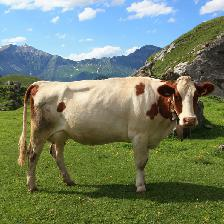
\includegraphics[width=\textwidth]{img/introduction/cow_original.jpg}
        \caption{Original}
    \end{subfigure}
    \hfill
    \begin{subfigure}[b]{0.22\textwidth}
        \centering
        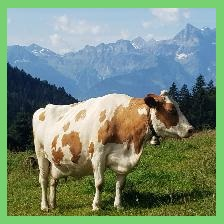
\includegraphics[width=\textwidth]{img/introduction/cow_noise.jpg}
        \caption{Sampling}
    \end{subfigure}
    \hfill
    \begin{subfigure}[b]{0.22\textwidth}
        \centering
        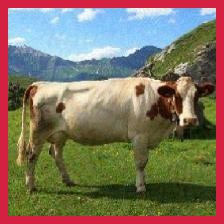
\includegraphics[width=\textwidth]{img/introduction/cow_fgsm.jpg}
        \caption{Adversarial}
    \end{subfigure}
    \hfill
    \begin{subfigure}[b]{0.22\textwidth}
        \centering
        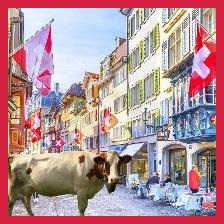
\includegraphics[width=\textwidth]{img/introduction/cow_ood.jpg}
        \caption{Distribution}
    \end{subfigure}
       \caption{Illustrative example of the three expected sources of variability. 
       A pre-trained MobileNetV2 model is shown to be vulnerable to adversarial perturbations 
       as the one represented in (c), and also to distribution shifts 
       as the one illustrated in (d), possibly because its inductive bias is influenced
       by the spurious correlation between cows and rural landscapes.}
       \label{fig:cows}
\end{figure}

This thesis will encompass all these phenomena under the same theoretical
framework, and devise a common approach to the measurement of
the shift entailed by both adversarial and distribution
variability sources. Robustness will be characterized from the space of
outcomes of the model, by means of a (posterior) probability 
distribution that will rank models and algorithms according to the
agreement in their predictions when facing different realizations of the same experiment.

\subsection{Adversarial setting}

As it was previously mentioned, certain perturbations on
original test images, which can be almost imperceptible
to the human eye, can lead to highly-confident but
incorrect predictions by deep neural networks, even when their
standard performance metrics are high.
Adversarial examples have been shown to transfer
across architectures and training procedures, and
even across subsets of data,
often yielding the same incorrect prediction in
all of these cases \cite{szegedyIntriguingPropertiesNeural2014}. \\

These intriguing phenomena were initially hypothesized to arise 
from a lack of smoothness over the input space, a property
commonly assumed in other learners, that derives from the
non-linear nature of deep learning architectures. Nevertheless,
extensive research on the field has elucidated that the root
cause is instead the linearity of its learning units, which makes them
vulnerable in certain directions of high-dimensional
spaces where small
effects can add up to significally change the outcome
\cite{goodfellowExplainingHarnessingAdversarial2015}. \\

Building on this intuition, numerous attacks have been proposed to evaluate the 
robustness of models against adversarial samples. A common strategy for inducing model 
failure involves identifying vulnerable directions in the feature space and adjusting 
perturbations to produce the desired misleading effect. Adversarial examples 
generated through these attacks can then be used to train robust models through 
regularization, thereby promoting generalization to the features present in 
worst-case examples and thus selecting models that are insensitivized
to them
\cite{baiRecentAdvancesAdversarial2021}.\\

Nevertheless, adversarial learning entails decision boundaries 
that are more complex than the ones derived via standard training
(see Figure \ref{fig:adversarial_complexity}), 
intuitively demanding more data and more complex 
architectures, at the risk of
overfitting to adversarial examples themselves
\cite{schmidtAdversariallyRobustGeneralization2018}. 
These limitations express a fundamental trade-off 
that arises from the intrinsic 
disparity between robust and non-robust features
\cite{tsiprasRobustnessMayBe2019, zhangTheoreticallyPrincipledTradeoff2019}. \\

\begin{figure}
    \centering
    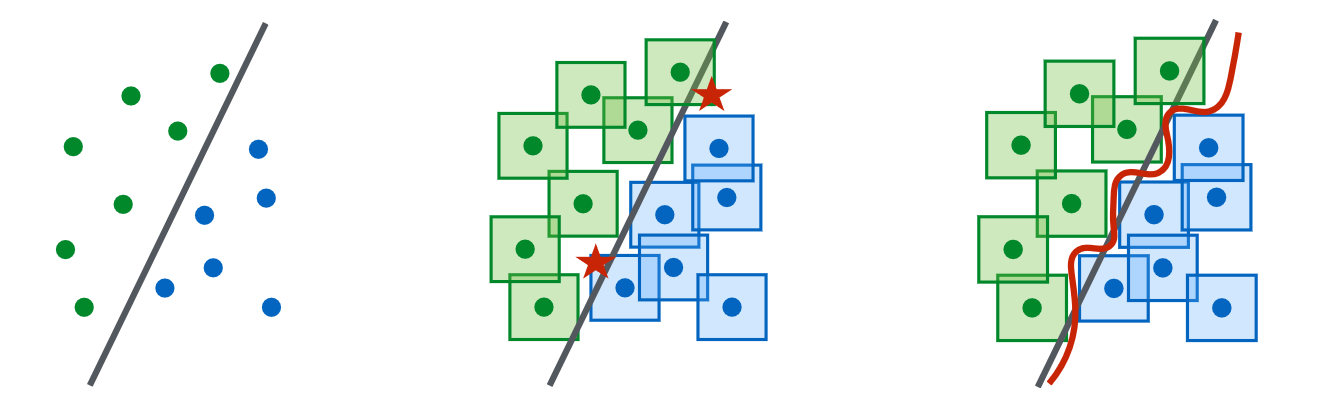
\includegraphics[width=0.65\textwidth]{img/introduction/adversarial_complexity.png}
    \caption{
    A conceptual illustration of standard vs. adversarial 
    decision boundaries. (\textbf{left}) A set of linearly-separable points. 
    (\textbf{middle}) Decision boundary learned via standard training.
    (\textbf{right}) Decision boundary learned via adversarial training.
    Both methods achieve zero training error, but only the robust model
    is able to generalize to $\ell_\infty$ perturbations.
    \cite{madryDeepLearningModels2019}
    }
    \label{fig:adversarial_complexity}
\end{figure}

Features selected via standard training
are the most predictive towards generalizing
to sampling randomness within the same dataset, but they do
not necessarily represent the features implicitly selected 
by humans and are not invariant to a human-based notion 
of similarity. Instead, features selected via adversarial training 
have been shown to better model this
invariance, and thus align much better with 
human perception, as seen in Figure \ref{fig:adversarial_loss}
\cite{ilyasAdversarialExamplesAre2019}. Furthermore, adversarial perturbations of robust 
models display salient characteristics;
that is, features that are perceived to belong to the
class they are misclassified to, as illustrated in Figure \ref{fig:salient_characteristics}
\cite{tsiprasRobustnessMayBe2019}. \\

\begin{figure}[H]
    \centering
    \begin{subfigure}[b]{0.28\textwidth}
        \centering
        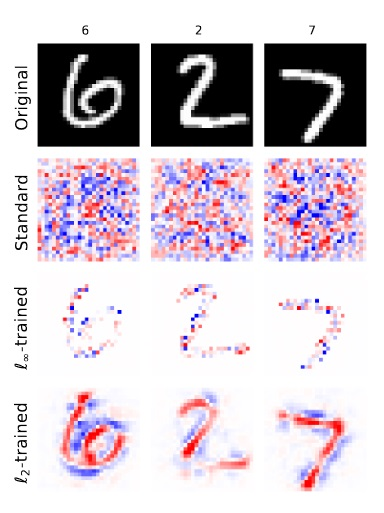
\includegraphics[width=\textwidth]{img/introduction/adversarial_loss_1.jpg}
        \caption{MNIST}
    \end{subfigure}
    \hspace{1cm}
    \begin{subfigure}[b]{0.28\textwidth}
        \centering
        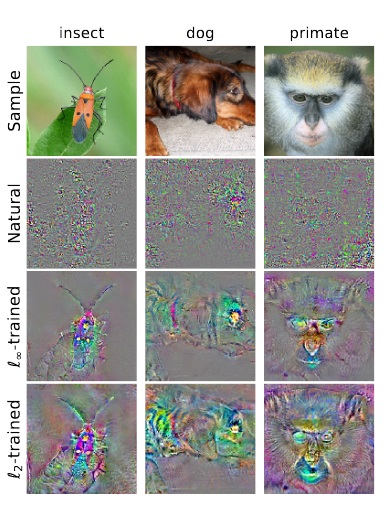
\includegraphics[width=\textwidth]{img/introduction/adversarial_loss_2.jpg}
        \caption{Restricted ImageNet}
    \end{subfigure}
       \caption{Scaled loss gradient with respect to input images.
       Input pixels yielding the highest predictive power are aligned 
       with perceptually relavant features for the case of adversarial
       models, while appearing completely random in the case of 
       standard models.
       \cite{tsiprasRobustnessMayBe2019}}
       \label{fig:adversarial_loss}
\end{figure}


\begin{figure}[H]
    \centering
    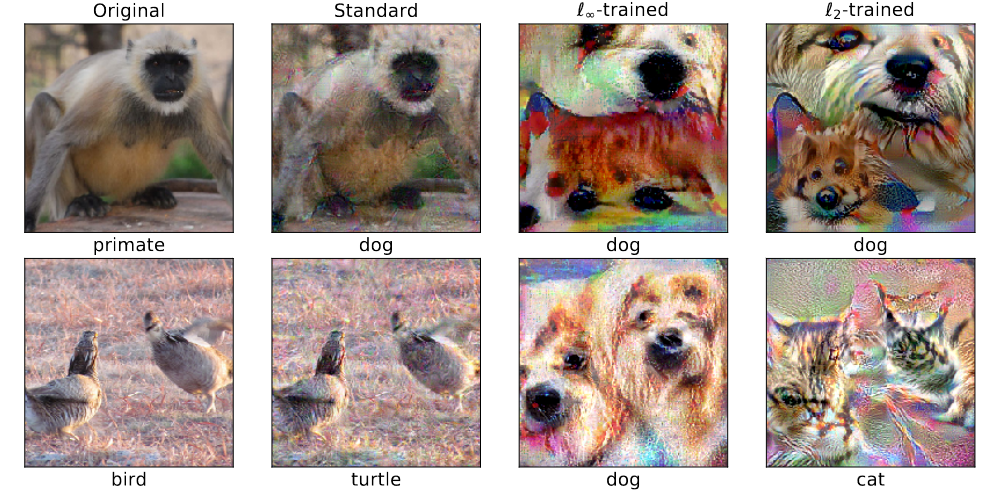
\includegraphics[width=0.45\textwidth]{img/introduction/adversarial_salient.png}
    \caption{Adversarial examples for standard and adversarially-trained models.
    Perturbed images produced for robust models 
    effectively capture salient data characteristics.
    % and appear similar to examples of a different class. 
    \cite{tsiprasRobustnessMayBe2019}}
    \label{fig:salient_characteristics}
\end{figure}

Overall, these and other findings suggest that robustness in the adversarial setting
is a fundamental property of the data features that are represented by models, 
rather than of the models themselves, and the phenomenon of transferability can be
explained in these terms. Training strategies that manage to navigate the 
robustness-generalization trade-off will be the ones yielding 
the best results, provided that the data distribution
is representative of the true underlying features. 

\subsection{Out-of-distribution setting}\label{sec:intro_ood}

Most learning algorithms work under the fundamental assumption that
a causal relationship exists between input and output spaces. The target function to 
learn represents that causality and must therefore remain 
invariant regardless of the available data, which implies that 
suitable approximations of this 
function can be obtained as long as data samples are independent 
and identically distributed in the input space
\cite{muandetDomainGeneralizationInvariant2013,quinonero-candelaDatasetShiftMachine2009}. 
Nevertheless, this is not always
the case, as often real-world data does not match the same statistical
patterns of the data used for training. Ultimately, this phenomenon induces a
distribution shift that leads to poor generalization performance
\cite{zhouDomainGeneralizationSurvey2022,wangGeneralizingUnseenDomains2022,liuOutOfDistributionGeneralizationSurvey2023}. \\

\begin{figure}[h]
    \centering
    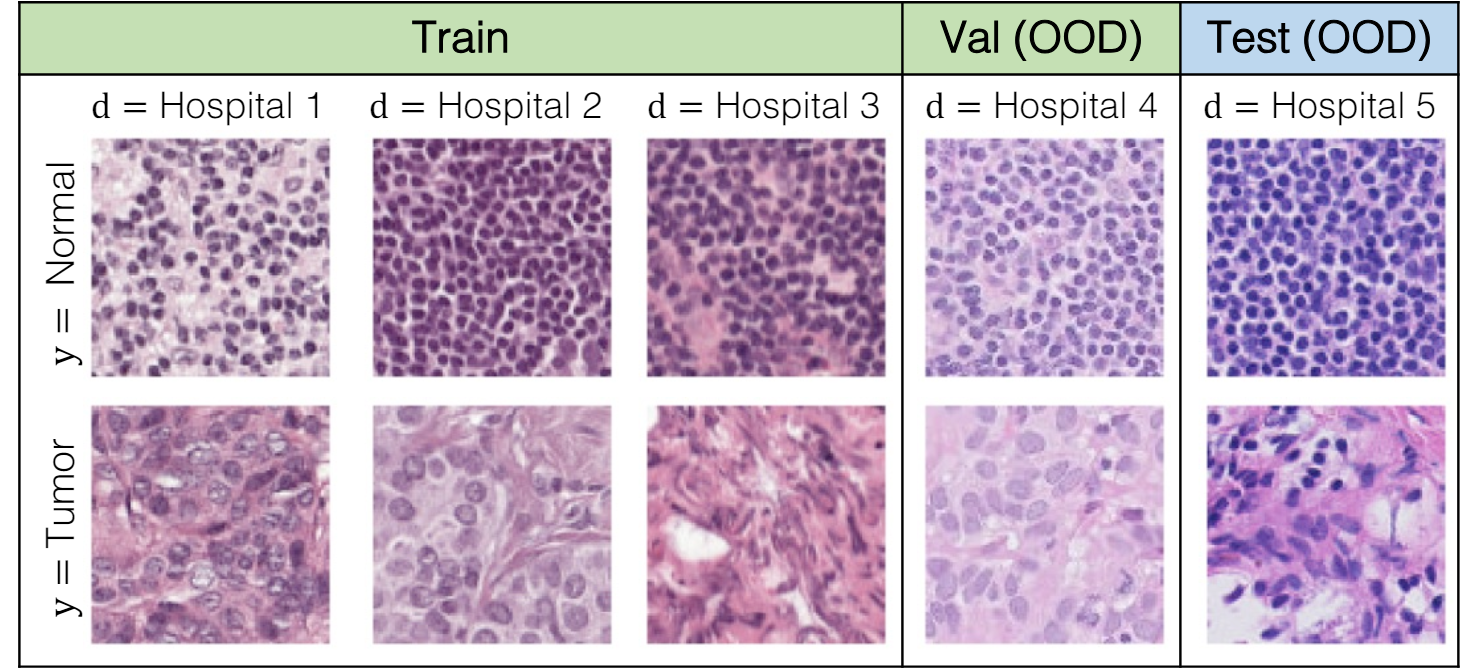
\includegraphics[width=0.5\textwidth]{img/introduction/camelyon17.png}
    \caption{The \texttt{camelyon17} (WILDS) dataset comprises images of stained 
    lymph node tissue patches sampled from different hospitals.
    \cite{kohWILDSBenchmarkIntheWild2021}
    }
    \label{fig:camelyon17}
\end{figure}

A distribution shift can arise for various reasons, namely the 
unfeasibility of collecting diverse enough data, the changing or time-dependent
nature of the data, or the implicit bias
introduced during the data collection process. This last case
is particularly relevant, as it can serve as a generalization of all
the previous cases and raise epistemological questions
about the learning framework itself. For instance, 
Figure \ref{fig:dataset_bias} refers to a cross-generalization analysis in which popular
machine learning datasets were shown to be biased towards
specific representation of features. Considering the fact that all
data is sampled from the same source (i.e. Internet), 
numerous human-induced biases are shown to determine the 
nature of representations, the most significant of all being 
negative bias, which arises when the negative subset\footnote{
    When certain observations in a dataset are labelled as belonging 
    to a specific class, the remaining observations are implicitly
    assigned to not belong to that class, and therefore define a
    negative set in the model's feature space.
}
of the dataset is not representative of the input subspace 
excluding that  particular class and results in a model that performs 
significantly worse in other datasets, even when trained with 
the same observations of that class.\\

\begin{figure}[H]
    \centering
    \begin{subfigure}[b]{0.35\textwidth}
        \centering
        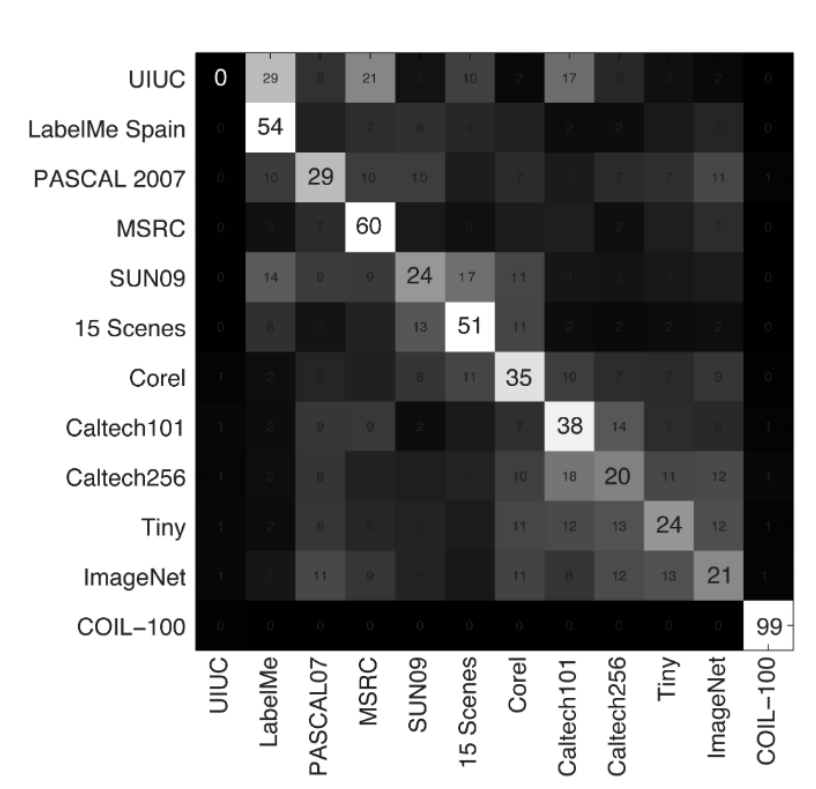
\includegraphics[width=\textwidth]{img/introduction/dataset_bias_confusion.png}
    \end{subfigure}
    \hspace{1cm}
    \begin{subfigure}[b]{0.32\textwidth}
        \centering
        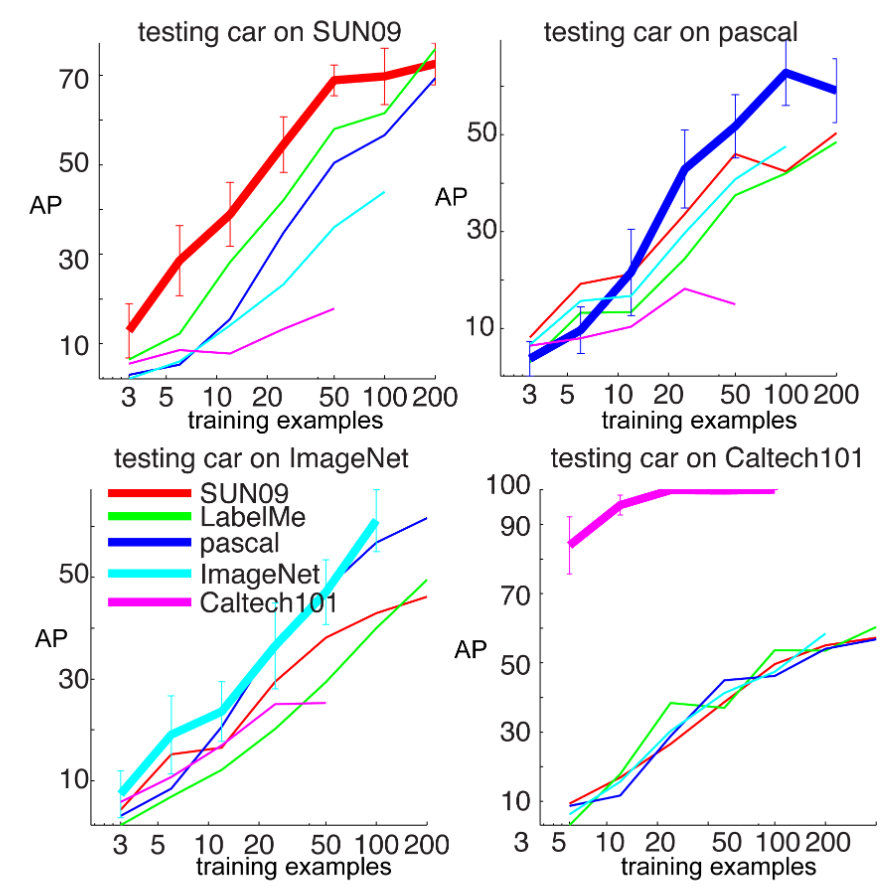
\includegraphics[width=\textwidth]{img/introduction/dataset_bias_cross_generalization.png}
    \end{subfigure}
       \caption{
        \textbf{(left)} Confusion matrix generated in a dataset
        identification task. A clearly pronounced diagonal 
        indicates that each dataset posesses unique traits that
        make it distinguishable from the rest.
        \textbf{(right)} Cross-dataset generalization
        for \texttt{car} detection as function of training data. 
        The vertical gap between lines represents the decrease in performance 
        when training on a different dataset, and the horizontal 
        shift corresponds to the increase in the amount of data needed 
        to reach the same performance.
        \cite{torralbaUnbiasedLookDataset2011}}
       \label{fig:dataset_bias}
\end{figure}

Several approaches can be taken to address this issue, depending
on the nature of the shift and the accessibility of the
causal structure of the data (see Figure 3 and Table 2 in 
\cite{wangGeneralizingUnseenDomains2022}).
Nevertheless, the common goal is to push the model towards
domain-invariant representations that foster robustness in the
face of distribution shifts, sometimes relaxing the causality condition
to an assumption of invariance or stability of the distribution in the output space
\cite{wangGeneralizingUnseenDomains2022,liuOutOfDistributionGeneralizationSurvey2023}. \\

In general, every formulation considers a set of source domains 
encompassing data that is available for the training of the model,
including any validation subsets used for model selection, 
regularization or hyperparameter tuning, and a set of target 
domains encompassing unseen data on which model performance will
be evaluated. Within this framework, a straightforward approach
to improving robustness is to directly sample target domains
and adjust feature representations to be invariant 
between both, which is commonly known as domain adaptation. \\

In this work we will focus instead on domain generalization, which 
refers to the case in which target domains are not accessible 
and feature invariance can be only enforced
from source domains
\cite{blanchardGeneralizingSeveralRelated}. In particular, two strategies will be considered, 
namely domain alignment and data augmentation/generation. \\

On the one hand, domain alignment stems from the target invariance hypothesis, 
and can be formulated as a regularization problem that pushes towards the 
minimization of the dissimilarity of feature  representations originated 
from different source environments. The feature space in which the 
alignment is performed (e.g. a kernel latent space, as Figure \ref{fig:dica} illustrates)
and the similarity metric considered will
determine the peculiarity of the method
\cite{shenWassersteinDistanceGuided2018,liangComprehensiveSurveyTestTime2023}. \\

\begin{figure}[H]
    \centering
    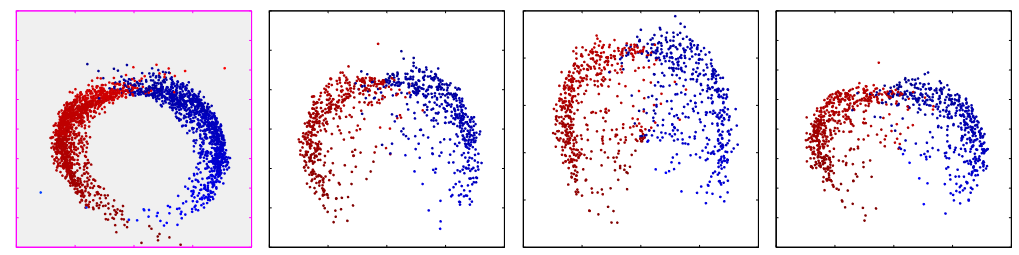
\includegraphics[width=0.65\textwidth]{img/introduction/dica.png}
    \caption{
    Projections of a binary synthetic dataset in the two principal DICA
    dimensions. The shaded box depicts the projection of training 
    data, whereas the unshaded boxes show projections of unseen 
    test datasets. \cite{muandetDomainGeneralizationInvariant2013}
    }
    \label{fig:dica}
\end{figure}

\begin{figure}[H]
    \centering
    \begin{subfigure}[b]{0.2\textwidth}
        \centering
        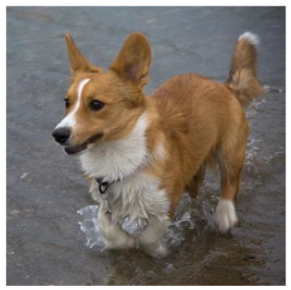
\includegraphics[width=\textwidth]{img/introduction/da_original.png}
        \caption{Original}
    \end{subfigure}
    \hspace{1cm}
    \begin{subfigure}[b]{0.2\textwidth}
        \centering
        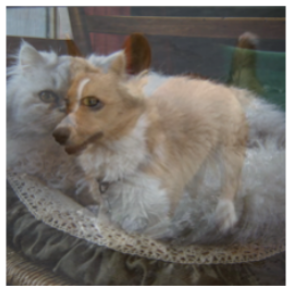
\includegraphics[width=\textwidth]{img/introduction/da_mixup.png}
        \caption{Mixup 
        \cite{zhangMixupEmpiricalRisk2018}
        }
    \end{subfigure}
    \hspace{1cm}
    \begin{subfigure}[b]{0.2\textwidth}
        \centering
        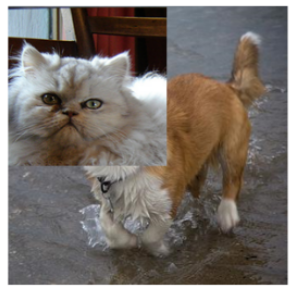
\includegraphics[width=\textwidth]{img/introduction/da_cutmix.png}
        \caption{CutMix
        \cite{yunCutMixRegularizationStrategy2019}
        }
    \end{subfigure}
       \caption{
        Mixup and Cutmix strategies can be used to interpolate
        between different labels and/or domains
        by generating intermediate observations.
        \cite{yunCutMixRegularizationStrategy2019}
        }
       \label{fig:data_augmentation}
\end{figure}

On the other hand, data augmentation/generation strategies 
do not need to assume target invariance and instead 
achieve cross-domain generalization by generating artificial observations that
diversify the original dataset with the hope of capturing 
the underlying causal structure of the data generation process. Augmented observations
can either be randomizations of original observations (e.g. transformations
such as rescaling or rotations) or new samples filling the distribution
gaps between domains (e.g. through interpolation, as illustrated 
in Figure \ref{fig:data_augmentation}). \\

Unlike in the adversarial setting, there is no common way of measuring
the shift in distribution betweeen source domains, and current approaches
are often constrained to specific datasets or training strategies. 
Robustness is instead quantified during (cross-)validation, either by reserving
a subset of each domain, leaving one domain out or
directly accessing target domains if they are available, 
which is known as the oracle approach. This last strategy is often
used to provide an upper bound estimate of model robustness, 
as it usually provides over-confident performance estimates
\cite{zhouDomainGeneralizationSurvey2022}.
Numerous benchmark datasets, some of which will be considered in this work, are the current 
standard for robustness assessment even with
the limitations they present
\cite{kohWILDSBenchmarkIntheWild2021}. 
\\

%Despite extensive research on the field and a wide variety
%of strategies envisionated, robustness to distribution shifts 
%continues to pose a fundamental challenge in machine learning. As
%previously mentioned, this difficulty primarily arises from the 
%violation of the sampling uniformity assumption, which renders 
%conventional learning techniques ineffective, and also from the 
%lack of a universal formal characterization of distribution shifts.
%Existing benchmark datasets, some of which will be considered in this work, are the current 
%standard for robustness assessment even with
%the limitations they present. \\

\section{Related work}

In the adversarial front, early work 
\cite{szegedyIntriguingPropertiesNeural2014}
unveiled the nature of the susceptibility of deep learning 
models to adversarial examples and FGSM 
\cite{goodfellowExplainingHarnessingAdversarial2015}
was introduced as an intuitive
approach for robust regularization. 
Since then, several gradient-based methods have been
proven to enhance adversarial robustness, such as PGD
\cite{madryDeepLearningModels2019}, C\&W 
\cite{carliniEvaluatingRobustnessNeural2017},
FMN
\cite{pintorFastMinimumnormAdversarial2021} and
many others (see 
\cite{liReviewAdversarialAttack2022} for reference). 
All of them ultimately entail a strategy to find
a vulnerable direction and adjust the perturbation 
(e.g. minimum-norm, maximum-confidence, etc.)
based on the location of the decision boundary, either via soft
constraints (i.e. regularization), boundary attacks or gradient
projections
\cite{baiRecentAdvancesAdversarial2021}. \\

In general, the primary distinction among adversarial attacks lies in
their knowledge of the model's architecture and parameters. In that
sense, white-box and black-box
attacks can be distinguished, where the former have full 
access to the model and the latter only 
to the model's predictions. In black-box settings, the loss gradient
is unknown and other strategies such as score-based or
decision-based attacks are used
\cite{liReviewAdversarialAttack2022}. Regarding adversarial training (i.e. defenses), 
robustness can
be achieved by a variety of methods, 
such as ensemble learning,
defensive distillation,
generative adversarial networks
\cite{xiaoGeneratingAdversarialExamples2019, miyatoVirtualAdversarialTraining2018},
diffusion models
\cite{wangBetterDiffusionModels2023,hoDenoisingDiffusionProbabilistic2020}
and adaptive-boundary methods
\cite{cohenCertifiedAdversarialRobustness2019}.
In this project, the Robustbench attack library
\cite{croceRobustBenchStandardizedAdversarial2021a}
will be leveraged to evaluate adversarial robustness 
in the CIFAR10 dataset
\cite{krizhevskyLearningMultipleLayers}. \\

In the domain generalization front, the existing rich taxonomy 
of methods can be classified into two main groups, namely
data manipulation and representation learning 
\cite{wangGeneralizingUnseenDomains2022,zhouDomainGeneralizationSurvey2022,liuOutOfDistributionGeneralizationSurvey2023}.
First, data manipulation strategies involve both augmentation and generation,
as for example image randomization or adversarial augmentation
\cite{yaoImprovingOutofDistributionRobustness2022,zhangMixupEmpiricalRisk2018,yunCutMixRegularizationStrategy2019}.
Second, representation learning strategies are primarily divided 
into domain-invariant methods (e.g. model-based
\cite{arjovskyInvariantRiskMinimization2020},
kernel-based
\cite{muandetDomainGeneralizationInvariant2013,arjovskyWassersteinGAN2017}
or adversarial-based
\cite{peiMultiAdversarialDomainAdaptation}) 
and feature disentanglement methods, which encompass causality-inspired
approaches and general multi-component analysis. Other 
learning strategies include meta-learning,
ensemble learning or self-supervised learning
\cite{liLearningGeneralizeMetaLearning2018,wangMetaFineTuningNeural2020}. \\

Regarding robustness characterization, a wide range of metrics
have been conceived (see
\cite{guoComprehensiveEvaluationFramework2023}), but
accuracy-based criteria are still the most common. As an alternative, 
some  theoretically-grounded approaches have been proposed, such
as CLEVER \cite{wengEvaluatingRobustnessNeural2018}, ACTS 
\cite{wangGeometricalApproachEvaluate2023}
or
PA
\cite{buhmannPosteriorAgreementModel2022}, 
which is the one explored in this work. 
In general, robustness is often reported and compared using 
robustness benchmark datasets. Some of the most relevant
for image classification tasks are 
MNIST 
\cite{lecun1998mnist}
(and its multiple variations, such as DiagVib-6
\cite{euligDiagViB6DiagnosticBenchmark2021}),
PACS
\cite{yuPACSDatasetPhysical2022},
VLCS
\cite{khoslaUndoingDamageDataset2012}
or WILDS
\cite{kohWILDSBenchmarkIntheWild2021}.

\section{Objectives}

The main goal of this project is to assess
the suitability of the posterior agreement framework in the 
context of deep learning model robustness for image 
classification tasks. For that, an operative version of posterior
agreement for finite, discrete hypothesis classes must be derived and
efficiently implemented, so that it can be used as a metric to evaluate 
and select models based on the robustness of their response to different 
sources and levels of randomness. The results obtained should be compared
with the current state-of-the-art in robustness evaluation, namely
Robustbench
\cite{croceRobustBenchStandardizedAdversarial2021a}
and WILDS 
\cite{kohWILDSBenchmarkIntheWild2021}
benckmarks in the adversarial and
out-of-distribution settings, respectively, and an overall
analysis of the use of the metric as an early-stopping 
criterion should be provided.\\

In order to conduct a comprehensive assessment, a series of steps should be undertaken in a 
deductive manner, so that evidence is provided starting from first principles and culminating
with performance evaluations on benchmark datasets. To begin with, the content of this work should
be self-contained, and for that a formal statement of the learning problem should be given. Both 
learning algorithms and classification models should be defined, including the nuances of their
parametrization via deep neural networks. \\

Next, the robustness challenge should be formulated within the framework of probability theory,
providing a rigorous mathematical foundation for understanding the principal sources of randomness that
are relevant in the context of this work. The generalization capabilities to specific sources of randomness
will determine the robustness score of a model, which for PA is conceived as a 
measure of the stability of the probabilistic output of the model to the randomness of the data 
sampling process. In this sense, the fundamental generalization-complexity trade-off must be reframed
within the context of information theory by relating complexity to the expected information content
of the data. The estimated informativeness will determine the resolution of the hypothesis space and
thus its stability under perturbations of various kinds. Once an operative PA metric is derived, 
its properties should be investigated and further assessed with artificial data, so that PA can be compared 
with baseline accuracy-based metrics at a fundamental level. \\

Experiments should be performed the adversarial setting first, for being adversarial perturbations
intentionally designed to change the prediction of the model and thus entailing a performance-based notion of
robustness that aligns with accuracy measures. After that, a customized implementation of 
the DiagVib-6 
\cite{euligDiagViB6DiagnosticBenchmark2021} 
syntetic data generation pipeline should be used to evaluate the suitability of PA in the domain
generalization setting. This will allow for a detailed analysis of the model selection capabilities of PA 
under different experimental conditions, especially regarding the source, power and rate of the shift 
entailed by each dataset and the accessibility of target domains for model validation and selection.\\


All in all, both analytical and numerical tools should be used to provide a comprehensive analysis
of the model-selection capabilities of PA and the source of its discriminative power. \\





\cleardoublepage
\chapter{Theoretical Background }\label{sec:theory}

\section{The learning framework}

Statistical learning theory encompasses the mathematical framework used to
study generalization in machine learning. In this formalism, the goal
is to learn a target function $f^*: \mathcal{X} \to \mathcal{Y}$ by means of an approximated
function $f \in \mathcal{F}$ using a finite set of observations. 

\begin{definition}[Supervised dataset]
    Let $\mathcal{X} \subseteq \mathbb{R}^d$ and $\mathcal{Y} \subseteq \mathbb{R}^t$ be
    the input and output spaces, respectively. Let $X$ be the random variable associated
    with the sampling in $\mathcal{X}$, and $\underbar{X} = (X_1, ..., X_N) \overset{\text{iid}}{\sim} X$ be a $N$-sized simple
    random sample of $X$. A supervised dataset $D$ is a realization of $\underbar{X}$ paired with its $f^*$-mapped output values.

    $$
    D = \{(\bm{x}_n, f^*(\bm{x}_n))\}_{n \in [N]}
    $$
\end{definition}

\subsection{Empirical risk minimization}

The quality of the approximation can be measured with the expected risk $\mathcal{R}(f)$

$$
\mathcal{R}(f)=\mathbb{E}_{x \sim X}[\mathcal{L}(f(x),f^\star(x))]
$$

where $\mathcal{L}: \mathcal{Y} \times \mathcal{Y} \to \mathbb{R}$ denotes a loss function. Glivenko-Cantelli theorem allow us to
estimate the expected risk with its empirical (plug-in) equivalent when $N$ is large enough.

\begin{definition}[Empirical risk] Let $D$ and $\mathcal{L}$ be the dataset and loss function of our problem, respectively. The empirical risk of $f \in \mathcal{F}$
    computed on $D$ is defined as

    $$
    \hat{\mathcal{R}}_D(f)=\frac{1}{N}\sum_{n=1}^{N}\mathcal{L}(f(\bm{x}_{n}),f^{\star}(\bm{x}_{n}))
    $$
\end{definition}

Training, therefore, amounts to minimizing the empirical risk over the function class $\mathcal{F}$.

$$
\text{ERM}_D = \hat{f}_D = \min_{f \in \mathcal{F}} \hat{\mathcal{R}}_D(f)
$$

The best learning algorithm will be that minimizing the difference between the 
expected and empirical risks computed on a different realization of the data. 

\begin{definition}[Empirical generalization error] Let $D_{t}$ and $D_v$ be two supervised datasets. Let $\hat{f}^* \in \mathcal{F}$ be the function minimizing the expected risk
    , and let $\hat{f}_{D_t}$ be the function minimizing the empirical expected risk computed on $D_t$. The empirical generalization error of $f_{D_t}$ computed on $D_v$ is defined as

    $$
    \mathcal{E}(D_t, D_v) = \hat{\mathcal{R}}_{D_v}(\hat{f}_{D_t}) = [\hat{\mathcal{R}}_{D_v}(\hat{f}) - \hat{\mathcal{R}}_{D_v}(\hat{f}^*)] + \hat{\mathcal{R}}_{D_v}(\hat{f}^*) = \mathcal{E}_{\text{estimation}}+ \mathcal{E}_{\text{capacity}}
    $$

    where $\mathcal{E}_{\text{capacity}}$ is governed by the ability of the function class $\mathcal{F}$ to represent the target function; i.e. its complexity.
\end{definition}


The definition of complexity depends on the problem, but intuitively measures the cardinality of the
subset of $\mathcal{F}$ that the algorithm is able to represent. A complex or high-capacity algorithm will
be able to represent a larger subset of $\mathcal{F}$ and achieve a low empirical error, but will be also
prone to overfitting to the specific learning realization thus yielding a higher generalization error. 

\subsection{Regularized risk minimization}

As a general principle, the inductive bias of the algorithm (i.e. the set of constraints imposed on $\mathcal{F}$ during learning) should be aligned with
that of our target function. Given that more expressive classes are always preferred by optimization algorithms, the ERM
objective function is usually tweaqued to include a regularization term penalizing complexity.

\begin{definition}[Regularized empirical risk] Let $\Omega: \mathcal{F} \to \mathbb{R}$ be a complexity measure. The regularized empirical risk of a function $f$
    computed on $D$ is defined as

    $$
    \hat{\mathcal{R}}_{\Omega}(f)=\hat{\mathcal{R}}(f) + \lambda \Omega(f)
    $$

    where $\lambda \in \mathbb{R}$ controls the trade-off between empirical risk and generalization error.

\end{definition}

The RRM problem now includes a hyperparameter $\lambda$, that will be selected so that the generalization error is minimized.

\section{Learning with neural networks}

Neural networks are biologically-inspired machine learning models that consist of a set of 
nodes (neurons) organized in layers and connected by weighted edges (synapses). Figure \ref{fig:nn_node} shows the 
data transformation performed by a single node.

\begin{figure}[H]
    \centering
    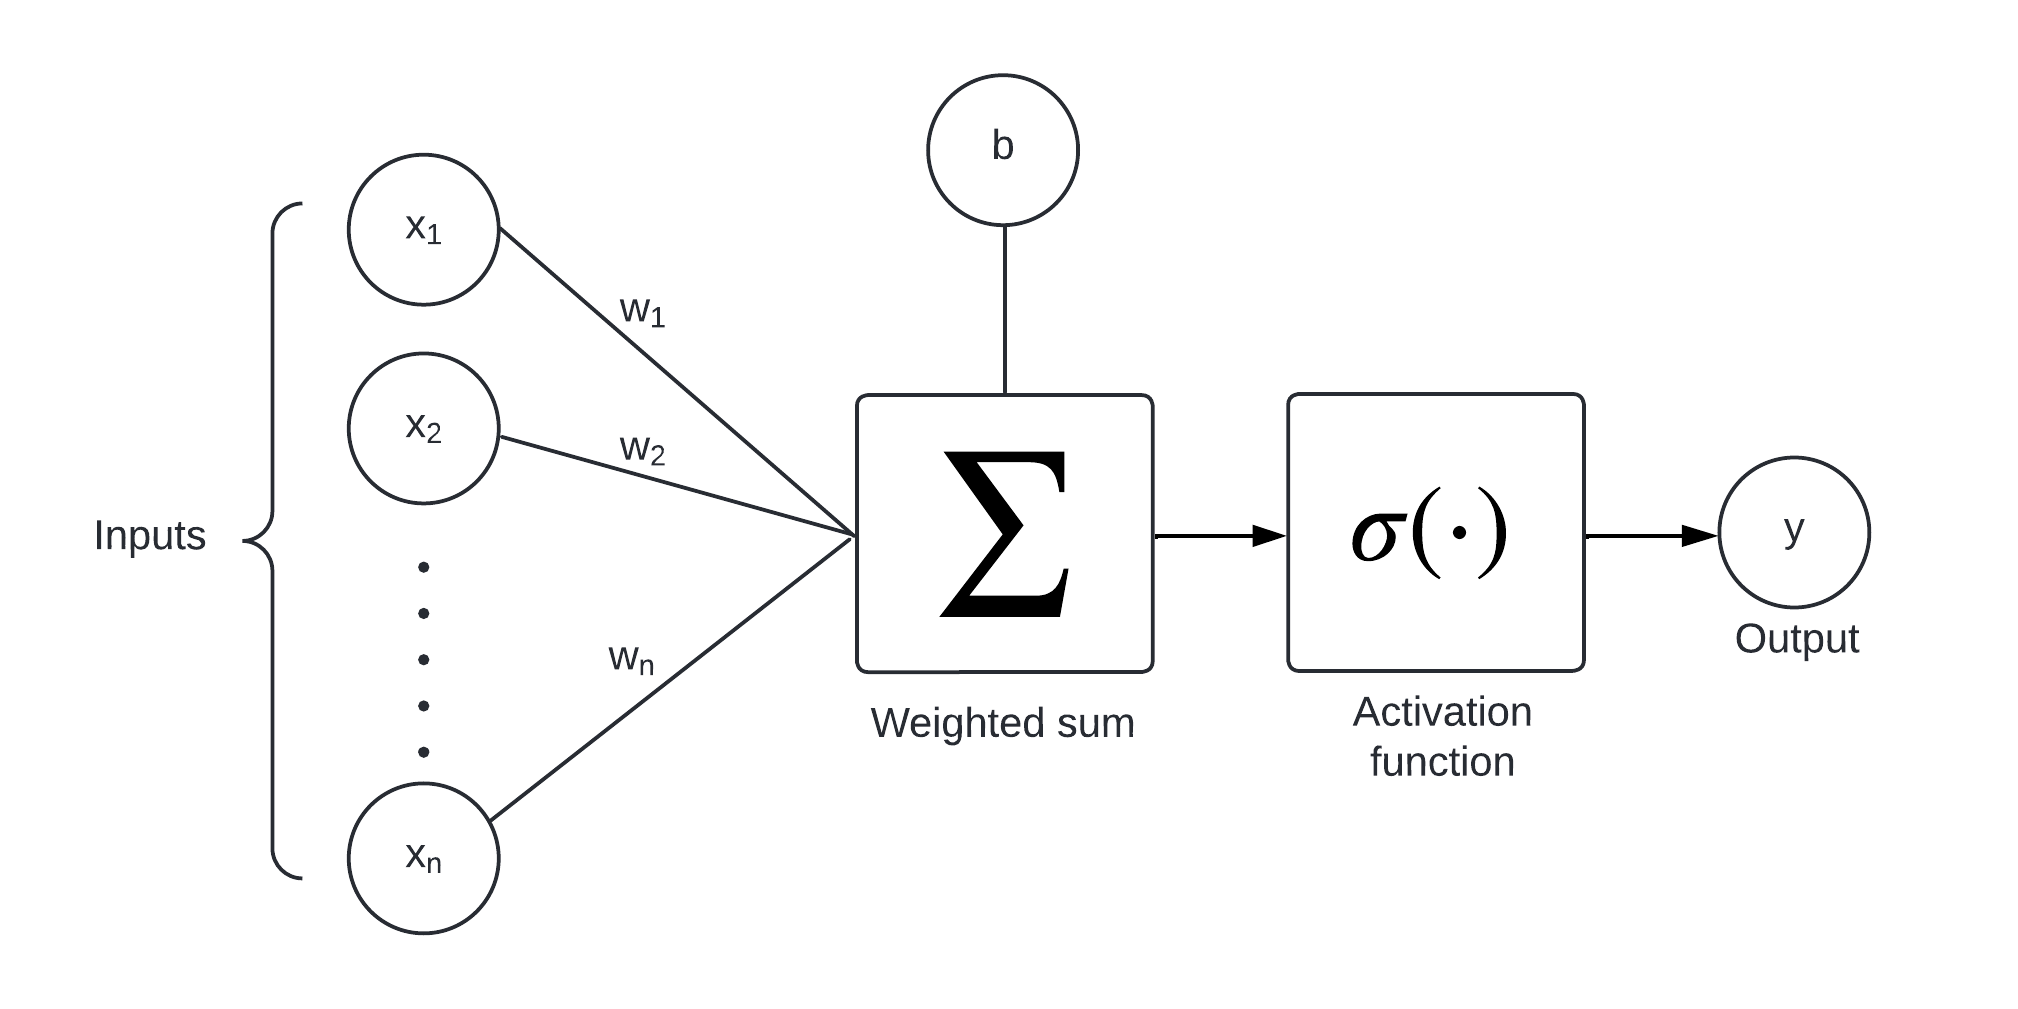
\includegraphics[width=0.4\textwidth]{img/theoretical_background/nn_node.png}
    \caption{The output of a node is computed by applying a non-linear
    activation function $\sigma(\cdot)$ to the weighted sum of its inputs.}
    \label{fig:nn_node}
\end{figure}

Let $\bm{x}_k \in \mathbb{R}^{d_k}$ be the input to the layer $k$, and let $\bm{W} \in \mathbb{R}^{d_k \times d_{k+1}}$ be the $k$-th weight matrix. The output of the layer can be expressed as

$$
\bm{x}_{k+1} = \sigma_k(\bm{z}_{k+1}) = \sigma_k(\bm{W}_k^T \bm{x}_k + \bm{b}_k)
$$

where $\sigma_k$ is the non-linear activation function at layer $k$. We can therefore express the overall transformation of a neural network
as the composition of its layers.

$$
f_{\text{NN}}(\bm{x}) = \bigcirc_{k=0}^{L-1} \sigma_k(\bm{W}_k^T \bm{x} + \bm{b}_k) = f(\bm{x}; \bm{\gamma})
$$

where $\bm{\gamma}$ represents the set of parameters of the network. In order to solve the learning problem, the optimization algorithm must navigate the non-convex loss
landscape towards the minimum of the empirical risk. This is computationally achieved by means of gradient-descent-based algorithms, which compute the
gradient over the parameters by means of the backpropagation algorithm.

\subsection{Backpropagation and gradient descent}

Let $w_{ji}^{(k)}$ be the weight from node $j$ on layer $k-1$ to node $i$ on layer $k$. Let $a_i^{(k-1)}$ be the output of node $i$ on layer $k-1$ and let $z_j^{(k)} = \sum_{i=0}^{n_k - 1} w_{ji}^{(k)} a_i^{(k-1)} + b_k^{(k)}$ be 
the linear input of node $j$ on layer $k$, so that $a_j^{(k)} = \sigma_j(z_j^{(k)})$ is the ouput from node $j$. We can compute the gradient of the loss $\mathcal{L}$ with respect to the weights by means of the chain rule as follows: 

$$  
\frac{\partial \mathcal{L}}{\partial w_{ji}^{(k)}} = \frac{\partial \mathcal{L}}{\partial a_{j}^{(k)}} \frac{\partial a_{j}^{(k)}}{\partial z_{j}^{(k)}} \frac {\partial z_{j}^{(k)}} {\partial w_{ji}^{(k)}} =
\frac{\partial \mathcal{L}}{\partial a_{j}^{(k)}} \frac{\partial \sigma_j^{(k)}}{\partial z_{j}^{(k)}} a_i^{(k-1)}
$$

Given that the loss is computed as a function of the output of the network, all the edges from node $i$ of layer $k-1$ influence the loss value at that node:

$$
\frac{\partial \mathcal{L}}{\partial a_{i}^{(k-1)}} = \sum_{j=0}^{n_{k} - 1} \frac{\partial \mathcal{L}}{\partial a_{j}^{(k)}}  \frac{\partial a_{j}^{(k)}}{\partial z_{j}^{(k)}} \frac{\partial z_{j}^{(k)}}{\partial a_{i}^{(k-1)}} =
\sum_{j=0}^{n_{k} - 1} \frac{\partial \mathcal{L}}{\partial a_{j}^{(k)}} \frac{\partial \sigma_j^{(k)}}{\partial z_{j}^{(k)}} w_{ji}^{(k)}
$$

All in all, we see that the same terms are required in different nodes to compute the gradient, making backpropagation algorithm very efficient. Equivalently, for the bias term:

$$
\frac{\partial \mathcal{L}}{\partial b_{j}^{(k)}} = \frac{\partial \mathcal{L}}{\partial a_{j}^{(k)}} \frac{\partial a_{j}^{(k)}}{\partial z_{j}^{(k)}} \frac {\partial z_{j}^{(k)}} {\partial b_{j}^{(k)}} = \frac{\partial \mathcal{L}}{\partial a_{j}^{(k)}} \frac{\partial \sigma_j^{(k)}}{\partial z_{j}^{(k)}}
$$

These derivatives are the components of the gradient vector that will be used to update the weights and biases of the network.

$$
w_{ji}^{(k)} = w_{ji}^{(k)} -\eta \frac{\partial \mathcal{L}}{\partial w_{ji}^{(k)}}
$$

$$
b_{j}^{(k)} = b_{j}^{(k)} -\eta \frac{\partial \mathcal{L}}{\partial b_{j}^{(k)}}
$$

where $\eta$ is the learning rate. More efficient variations of gradient descent such as stochastic gradient descent or Adam are used in practice.


\subsection{Loss landscape and parameter space}


A neural network architecture $\text{NN}$ can be expressed as a parametrization of the function space $\mathcal{F}$.

$$
    \begin{aligned}
        \text{NN}: \bm{\Gamma} & \subseteq \mathbb{R}^{S} \longmapsto \mathcal{F}_{\bm{\Gamma}} \\
        \bm{\gamma} & \longmapsto f(\bm{x}; \bm{\gamma}) = f_{\text{NN}}(\bm{x})
    \end{aligned}
$$

where $\Gamma$ is the parameter space associated with this particular architecture. The functional
landscape $\mathcal{F}_{\bm{\Gamma}}$ consists of all mappings $f(\bm{\gamma}): \mathcal{X} \longmapsto \mathcal{Y}$ that 
that can be realized by some parameter configuration $\bm{\gamma} \in \bm{\Gamma}$. \\

Universal approximation theorems state that arbitrarily wide or abitrarily deep architectures
are able to represent virtually any function, but it is an open challenge to theoretically describe which
complexity measure regulates generalization. A possible approach to this problem is to
study the geometry of the loss landscape, especially in the vicinity of local minima. For instance, 
connected flat minima are often linked to better generalization capabilities, as they
intuitively represent a robust manifold in the parametrization space and should be preferred over sharp minima. \\

In this work we will explore a different approach to the generalization problem, based on
a definition of the generalization error that relies on the implicit randomness of the
data sampling process. 

\section{Generalization error}

As we mentioned in the first lines of this chapter, the input of learning algorithms are
realizations of the random variable $X$ defined over the input space $\mathcal{X}$. The
implicit randomness embedded in the sampling process extends to the outcome of algorithms,
even when performing a deterministic sequence of operations. An alternative intuition of 
generalization arises from this perspective, in the sense that a learning algorithm should
learn the same function $f$ when trained on different realizations of the same experiment. This
intuition will be formalized in this section.\\

\subsection{Posterior distribution}

The function $f \in \mathcal{F}$ was defined mapping $\mathcal{X} \longmapsto \mathcal{Y}$, in the sense that an observation $x \in \mathcal{X}$ is mapped to
a prediction $f(x) \in \mathcal{Y}$. In order to formalize the randomness of the data sampling process, we
will redefine $\mathcal{X}$ so that its elements are realizations of the simple 
random sample $\underbar{X}$, which are then mapped to a set of outcomes $\theta$.

\begin{definition}[Distribution of $\underbar{X}$]
    The simple random sample $\underbar{X} \overset{\text{iid}}{\sim} X$ has a probability distribution
    described by the density function $f_{\underbar{X}}$.

    $$
     f_{\underbar{X}} = \prod_{n=1}^{N} f_{X}(x)
    $$

    We will refer to this probability distribution as $\mathbf{P}_X$ to avoid notation clutter.
\end{definition}

\begin{definition}[Hypothesis class]
    A data science algorithm learns a function $f$ implementing the following mapping:

    $$
    \begin{aligned}
        f: \mathcal{X} & \longmapsto \Theta \\
        \bm{x} = (x_1, \dots, x_N) \sim X  & \longmapsto (f(x_1), \dots, f(x_N)) = \theta
    \end{aligned}
    $$

    The output space of hypothesis $\Theta$ represents all possible outcomes of a function
    $f$ learned on a dataset sampled from $\mathcal{X}$.

\end{definition}

Intuitively, this framework interprets complexity from the perspective of the possible
set of outcomes of the function, rather than the function class itself. It can be argued
that both perspectives are equivalent, in the sense that the function class can be mapped 
to the hypothesis space $\Theta$. Nevertheless, more suitable generalization regularization
constraints can be defined in $\Theta$, especially when dealing with intractable
function classes $\mathcal{F}_{\Gamma}$ derived from deep neural networks. \\

For instance, complexity in the hypothesis class can be associated to the nature of the
randomness displayed by $X$. Ideally, too restrictive hypothesis classes that lack desirable
hypothesis for some realization $\bm{x}$ of $\underbar{X}$ should be avoided, and also those hypothesis
classes containing unrealizable elements (i.e. hypothesis that are not outcome of
any possible experiment). A richness condition can thus be postulated following
this intuition. \\

\begin{definition}[Richness condition]
    Let $\tau \in \mathbb{T}$ be a transformation of the sampling experiment $X$. The dependency
    of the data on the experimental design will be captured by the index $\tau$, and we will
    implicitely consider $\underbar{X}$ to be a sample of $\tau \circ X$.  We require a
    sufficiently rich set of experiments $\mathbb{T}$ such that every hypothesis $\theta \in \Theta$
    is the (most likely) outcome of some realization $\bm{x}$.

    $$
    \forall \theta, \exists \tau \in \mathbb{T} \text{ such that } f(\bm{x}) = \theta
    $$
\end{definition}


Since we assume a mapping $f$ and a data distribution $\mathbf{P}_X$, we can describe
the randomness of the hypothesis outcome conditioned on the the distribution of the data.

\begin{definition}[Posterior]
    A probability distribution over the hypothesis class can be defined as a 
    conditional distribution given an realization $\bm{x}$ of experiment $\underbar{X} \sim \mathbf{P}_X$. We will
    refer to this distribution as the posterior over $\Theta$ under $f$.

    $$
        \begin{aligned}
            f: \mathcal{X} \times \Theta & \longmapsto \mathbb{R} \\
            (\bm{x}, \theta) & \longmapsto \mathbf{P}^f (\theta \mid \bm{x})
        \end{aligned}
    $$

    $\mathbf{P}^f$ establishes the stochastic relation between data and hypothesis.
    
\end{definition}

Using these definitions we can operate over $\Theta$ within the framework of probability 
theory. For instance, we can obtain the (prior) probability of a hypothesis to be
selected by $f$ given $\underbar{X}$ as

$$
 \Pi^f (\theta) = \mathbb{E}_X \mathbf{P}^f (\theta \mid \bm{x})
$$

from which we can derive a probabilistic version of the richness condition, where a limit
case can be imposed with exactly one experiment per hypothesis, leading to a uniform prior:

$$
\Pi^f (\theta) = |\Theta|^{-1}
$$

Within this framework, selecting suitable hypothesis classes amounts to selecting
posterior distributions that yield a higher probability to the desired subset of hypothesis. This
is the leading principle that will guide the derivations that follow.

\subsection{Generalization error}

In order to define a generalization error within this framework, we will proceed in an
analogous way as we did in the previuous section. We will consider two datasets $D_t$ and $D_v$
that arise from two different sampling realizations. In this case, however, we will make
explicit the fact that they encode different instantiations of the randomness associated
with the sampling, and thus denote $\bm{x'}$ and $\bm{x''}$ as realizations of the two simple random
samples $\underbar{X}', \underbar{X}'' \overset{\text{iid}}{\sim} X \mid \tau$, respectively, and associate
each dataset with one of them. The $\tau$ indexing is now explicit, since both samples are conditionally
independent given the experiment:

$$
    \mathbf{P}(\underbar{X}', \underbar{X}'') = \mathbf{P}(\underbar{X}' \mid \tau) \mathbf{P}(\underbar{X}'' \mid \tau)
$$

The selection principles for a posterior distribution will be the following:
\vspace{-2mm}
\begin{description}
    \item[P1] It should be expressive enough to cover the realizable $\Theta$.
    \vspace{-3mm}
    \item[P2] Equally likely inputs drawn from the same experiment should yield similar sets of hypothesis.
\end{description}

\begin{definition}[Description length]
    Let $\mathcal{F}_{\bm{\Gamma}}(\cdot)$ be the function class containing all functions 
    represented by the parametrization $\bm{\Gamma}$. Let $\mathbf{P}_{\bm{\Gamma}}$ be the
    universal distribution relative to $\mathcal{F}_{\bm{\Gamma}}$ fulfilling the minimum
    description length principle. The description length of a function $f_\gamma \in \mathcal{F}_{\bm{\Gamma}}$ 
    is defined as the number of bits required to encode its parameters. The code length
    of the argument of such distribution is

    $$
    \text{DL}_{f_{\gamma}}(\cdot) = -\log f_{\gamma}(\cdot)
    $$
\end{definition}

The quality of the represented function $f$ will be measured by the description
length of its posterior, and thus a loss function can be defined as follows.

$$
    \ell (\theta, \bm{x}) = - \log \mathbf{P}^f (\theta \mid \bm {x})
$$



Given that the description length encompasses also the complexity of the hypothesis
class and not only the generalization capabilities, we will normalize the loss dividing by the
description length of the prior.

$$
    - \log \Pi^f (\theta) = - \log \mathbb{E}_X \mathbf{P}^f (\theta \mid \bm{x})
$$

\begin{definition}[Generalization error]
    Let $\bm{x'}$ and $\bm{x''}$ be realizations of $\underbar{X}', \underbar{X}''$, respectively.
    Let $\Theta$ be the hypothesis class represented by $f$ given data $X$. The generalization error 
    in the support $\mathcal{X}$ is defined as the out-of-sample description length:

    $$
        \mathcal{G}_{\mathcal{X}} = \mathbb{E}_{X', X''} \mathbb{E}_{\theta \mid X'} \left[ - \log \frac{\mathbf{P}^f(\theta | \bm{x}'')}{\Pi^f (\theta)} \right]
    $$
    
\end{definition}



It amounts to the expected normalized loss over the validation data $\bm{x}''$ computed
over the distribution on the hypothesis expressed by the posterior on the training data $\bm{x}'$.
Intuitively, a lower generalization error is achieved when good quality posteriors on $\bm{x}''$ are 
assigned a high probability by the posterior on $\bm{x}'$. 

\begin{lemma}[Posterior agreement]
    The generalization error $\mathcal{G}_{\mathcal{X}}$ is non-negative and has a lower bound $-\mathcal{J}$. We define $\mathcal{J}$ as the posterior agreement.
\end{lemma}
\begin{proof}
    $$
    \begin{aligned}
        \mathcal{G}_{\mathcal{X}} & \geq \mathbb{E}_{X', X''}\left[-\log \left(\mathbb{E}_{\theta \mid X'} \frac{\mathbf{P}^{f}\left(\theta \mid \bm{x}''\right)}{\Pi^{f}(\theta)}\right)\right] \\
        & =\mathbb{E}_{X', X''} \left[-\log \left(\sum_{\theta \in \Theta} \frac{\mathbf{P}^{f}\left(\theta \mid \bm{x}'\right) \mathbf{P}^{f}\left(\theta \mid \bm{x}'' \right)}{\Pi^{f}(\theta)}\right)\right] = -\mathcal{J} \\
        & \geq-\log \left(\mathbb{E}_{X', X''} \mathbb{E}_{\theta \mid X'} \mathbb{E}_{\theta \mid X''} \frac{\mathbf{P}^{f}\left(\theta \mid \bm{x}''\right)}{\Pi^{f}(\theta)}\right)=0 .
    \end{aligned}
    $$
\end{proof}

where Jensen's inequality has been applied twice to the convex function $-\log(\cdot)$:

$$
    \log (\mathbb{E} [\cdot]) \leq \mathbb{E}[\log( \cdot)]
$$

\subsection{Maximum posterior agreement}

Describe max posterior agreeement problem. All Joachim, but be brief.

\section{Posterior agreement kernel}

\subsection{Classification problem}

Statement of the classification problem. Follow structure from 


\section{DS algorithms, NNs and distribution shift}
MOST COMPLICATED SECTION. \\
- Cite Joachim, introduction to DS algorithms. Introduce notation that will follow the
rest of the thesis. Particularize for NNs (work to do).\\
- Explain function representation problem in NNs, why it is important. (look at phd zotero) \\
- Read about info theory, why description length  \\
- Start with two datasets, training and validation, and their distributions (also Joachim) \\
- Derive the OOD-error from the previous theory. More detail than Joachim. \\

\section{From OOD error to PA}
- Definitions and proofs (ommitted by Joachim) that lead to PA \\
- Intuition behind PA, plot. \\
- Read more about previous work from Joachim, where PA has worked. \\
- Include (briefly) the binary symmetric channel as an example, as it is 
important for Joachim and will be referenced later. \\

\section{The PA kernel}
- Follow derivation overleaf, include factorization theorem. \\
- Explain change of perspective, think of (binary) classification as a binary
symmetric channel. \\

\subsection{Properties}
(all in overleaf or papers) \\
- Positive definiteness, explain why important \\
- Symmetry, explain why important \\
- Convexity analysis. \\
- Problem with binary classification \\

\subsection{Example}
- Analytical results obtained, overleaf. \\


\section{Generalization error in the hypothesis space}
- Alternative formulation \\
- Explain why important, and formalize the data augmentation strategy (presentation) \\


\cleardoublepage
\chapter{Results and discussion}\label{sec:results}

The fundamental goal of this project is to assess the suitability of posterior
agreement as a robust model selection criterion in the image classification setting.
This section will outline the principal results in a deductive way, starting with an 
empirical exploration of the robustness properties of the PA kernel and culminating
with performance results in benchmark datasets.

\section{PA as a robustness metric}\label{sec:results_robustness}

\subsection{Empirical behaviour}

Starting from the simplest possible setting, we will explore the behavior of the metric 
under different levels of sample mismatch. More specifically, we will assess the performance 
of perfect, random, and constant binary classifiers by manipulating a 
Bernoulli sample and simulating different levels of prediction confidence.

\begin{figure}[H]
    \centering
    \begin{subfigure}[b]{0.45\textwidth}
        \centering
        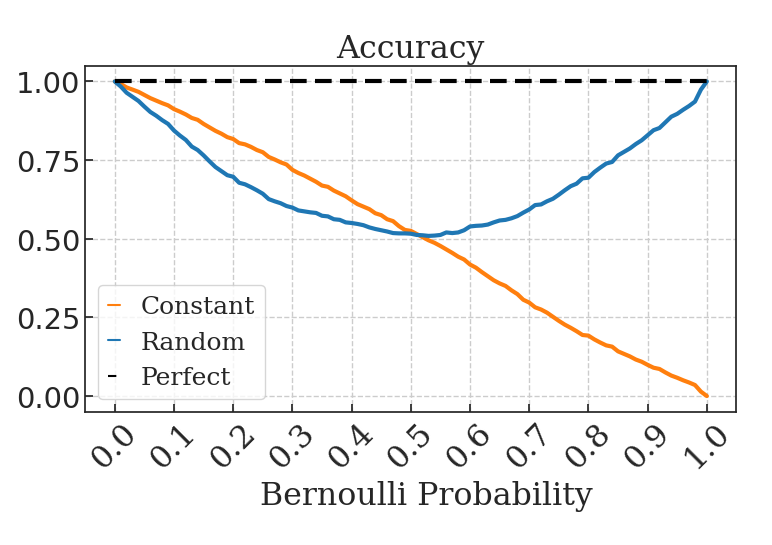
\includegraphics[width=\textwidth]{img/results_discussion/empirical/artificial_acc_final.png}
    \end{subfigure}
    \hfill
    \begin{subfigure}[b]{0.45\textwidth}
        \centering
        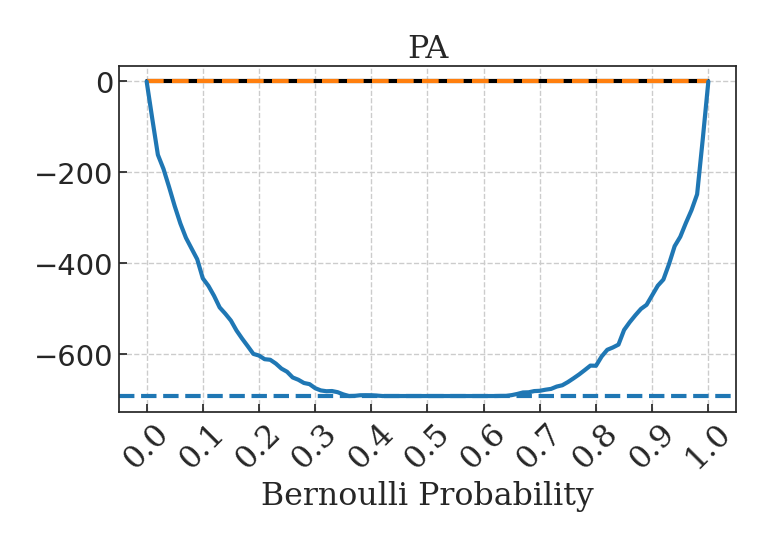
\includegraphics[width=\textwidth]{img/results_discussion/empirical/artificial_logPA_final.png}
    \end{subfigure}
    \caption{Evolution of performance and robustness for the three classifiers}
    \label{fig:empirical_plot}
\end{figure}

A $N=1000$ Bernoulli sample was generated with a symmetrical confidence level 
of prediction $\pm \Delta/2$. For $p=0.5$, the metric achieves its minimum 
value $N \log{1/2}$ for the random classifier, as $\beta = 0$, and tends to its maximum
value of $0$ as $\beta \longrightarrow \infty$.

\begin{table}[H]
    \centering
    \begin{tabular}{lccc}
    Classifier & Accuracy & $\beta$ & PA \\
    \midrule
    Perfect   & 1.000     & 12.331  & $-0.0088218$ \\
    Constant  & 0.525     & 12.331  & $-0.0088218$ \\
    Random    & 0.516     & 0.000   & $-693.14$    \\
    \bottomrule
    \end{tabular}
    \caption{Comparison of classifier performance metrics for $p = 0.5$.}
    \label{tab:empirical_table}
\end{table}

The random classifier sample was generated by permuting the original so 
that the number of mismatched observations depends on the bernoulli probability $p$. 
As we can see, the theoretical miniumum value  is obtained only after
a certain perturbation threshold has been reached. This illustrates the trade-off
navigated during the kernel optimization, in which matching samples penalize the 
metric value the lower the value of $\beta$ is, whereas mismatching samples will
penalize the overall value the further from zero $\beta$ is. Given the highly non-linear
nature of the logarithm in the interval $[0,1]$, the metric will penalize 
disagreement much more than agreement, as shown in Figure \ref{fig:empirical_plot}.
A truly random classifier (i.e. balanced on the two classes) would yield the minimum
PA value for any possible original sample, as shown in the blue dashed line.\\

One of the most relevant differences between posterior agreement and any accuracy-based
measure, as discussed in previous chapters, is the fact that its assessment is based on
the whole probabilistic output of the model, and therefore can be used as a measure of
confidence in the predictions. The prediction confidence, expressed as a difference in 
the unnormalized log-odds (commonly known as logits), is very informative with regard 
to the quality of the model, as we can intuitively infer that the latent 
space represented by a high-confidence model encodes a better set of features 
to discriminate observation classes than one with a lower prediction confidence. \\

For instance, when comparing two models of similar predictive power but at different 
confidence levels, maximum posterior agreement will be achieved with a higher 
$\beta^{*}$ for the model that tends to yield more flattened distributions. This
information is especially valuable in the covariate shift setting, given that robust
models that rely on less accessible sets of features will most likely yield conservative
predictions on in-distribution samples, but at the same time keep a high prediction
power on out-of-distribution observations. \\

\begin{figure}[H]
    \centering
    \begin{subfigure}[b]{0.45\textwidth}
        \centering
        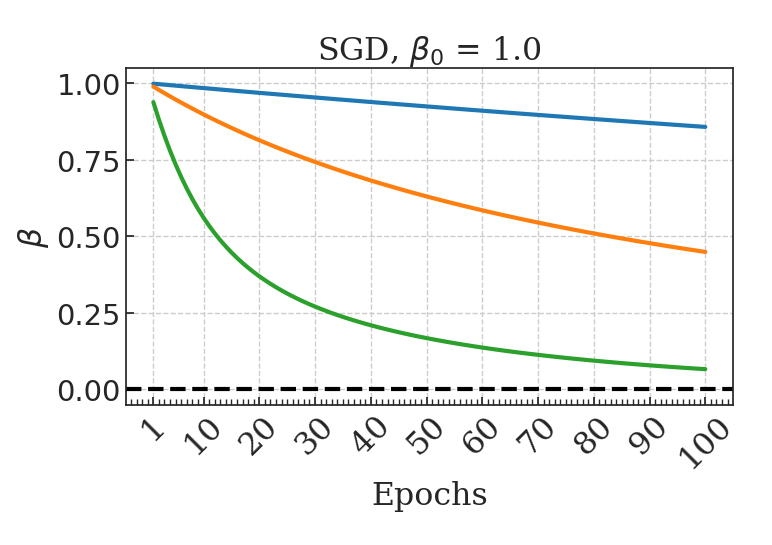
\includegraphics[width=\textwidth]{img/results_discussion/empirical/nonrob_met=betas_hue=ldiff.png}
    \end{subfigure}
    \hfill
    \begin{subfigure}[b]{0.45\textwidth}
        \centering
        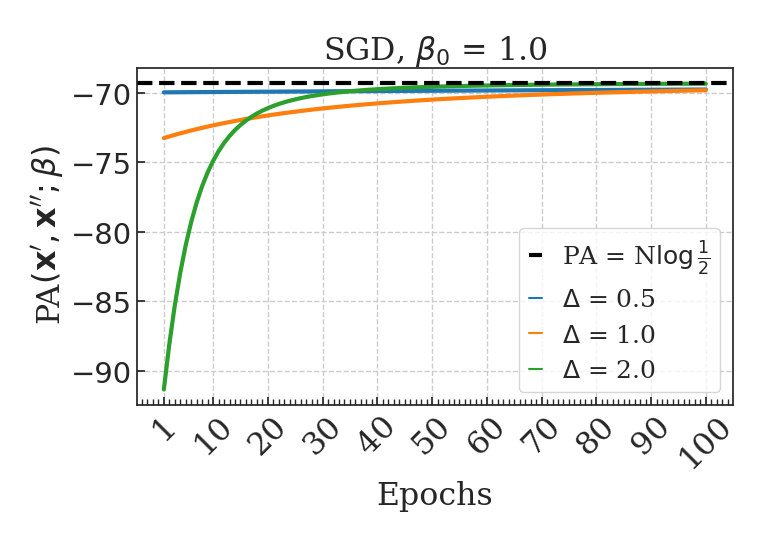
\includegraphics[width=\textwidth]{img/results_discussion/empirical/nonrob_met=logPA_hue=ldiff.png}
    \end{subfigure}
    \caption{Evolution of PA kernel optimization under different levels of prediction 
    confidence. An illustration of the original log-odds and its associated posterior distribution
    can be found in Appendix \ref{subsec:appendix_empirical_behaviour}.}
    \label{fig:prediction_confidence}
\end{figure}

These and other results (see Appendix \ref{subsec:appendix_empirical_behaviour}) indicate
that the PA kernel behaves as expected and is highly informative of the generalization
capabilities of the model, provided that the nature of the randomness existing
between $\bm{x}^\prime$ and $\bm{x}^{\prime \prime}$ is known.

\subsection{Robustness assessment to sampling randomness}

The results obtained with artificial samples motivate the exploration of more realistic
scenarios. In general, the PA metric is expected to capture the generalization capabilities
of any model yielding probabilistic predictions, regardless of the task at hand. This
already represents an incredible advantage from an epistemological perspective, as we
can argue that the metric is agnostic of the underlying mechanism that generated the data
and even to the nature of the data itself. \\

In order to verify this claim, we will start by evaluating the robustness of two
different classifier models in two different domains under increasing levels of 
white noise perturbation. This particular setting, even if highly artificial, is 
relevant in any classification context, as it represents general measure of the 
quality of the features learned by the model. The presence of white noise, at least 
at low levels, does not perturb the set of features that define a particular class from
a human perspective, and should therefore not perturb very significantly the
predictions yielded by the model. \\

HERE THE PLOT OF THE LEVENSHTEIN DISTANCE PLOT HERE. \\

A sentiment classifier analysis. In this case, the random nature of the noise perturbations
is shown to exploit specific vulnerabilities of language models, which paradoxically 
have been shown to be robust to more highly crafted perturbations, such as changes in
language or replacement of complete words. \\

\begin{figure}[H]
    \centering
    \begin{subfigure}[b]{0.45\textwidth}
        \centering
        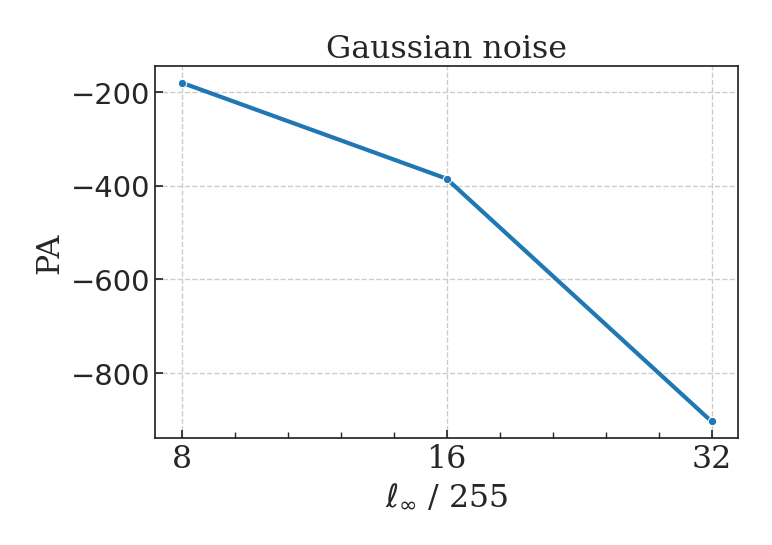
\includegraphics[width=\textwidth]{img/results_discussion/adversarial/GAUSSIAN_logPA_eps_single.png}
    \end{subfigure}
    \hfill
    \begin{subfigure}[b]{0.45\textwidth}
        \centering
        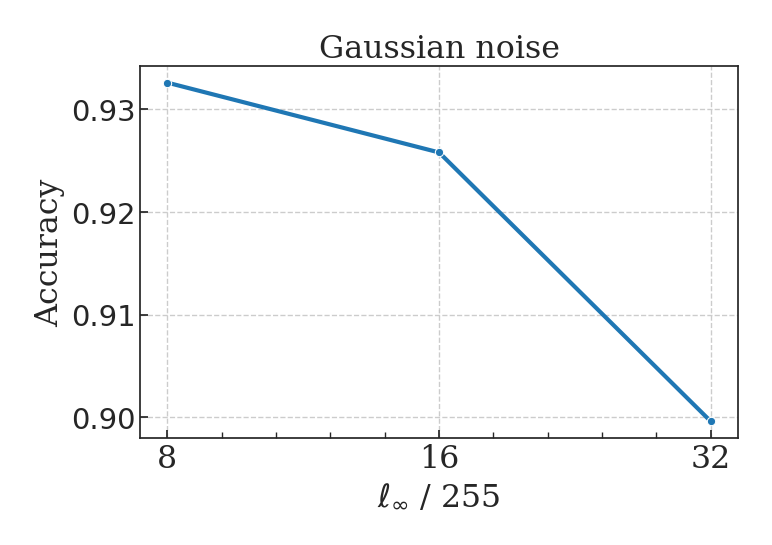
\includegraphics[width=\textwidth]{img/results_discussion/adversarial/GAUSSIAN_acc_pa_eps_single.png}
    \end{subfigure}
    \caption{PA and accuracy of CIFAR10 classification for increasing levels of white noise intensity.}
    \label{fig:gaussian_noise}
\end{figure}

In this second example, a 10.000 observation sample of CIFAR10 images was perturbed
with white noise at different levels of intensity. The magnitude of the perturbation
is expressed in the same terms as those of an adversarial 
attack (see Section \ref{sec:adversarial_setting}) for further 
reference, but translate to using $\sigma = 3 \ell_\infty$, as 99.73\% of the
total mass of the gaussian distribution lies within the interval $\pm 3\sigma$. \\

As expected, PA is highly sensitive to the presence of white noise,
and is able to capture the generalization capabilities of the model in a much more
informative way than accuracy. We can obtain a higher understanding of the degree of
sensitivity of the metric if we adjust the perturbation so that if only affects
a certain ratio of observations. \\

\begin{figure}[H]
    \centering
    \begin{subfigure}[b]{0.49\textwidth}
        \centering
        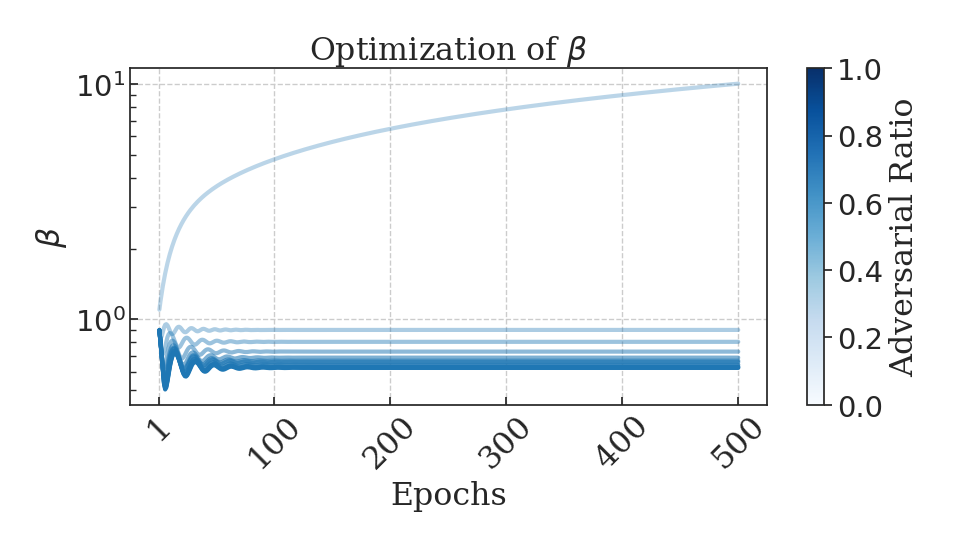
\includegraphics[width=\textwidth]{img/results_discussion/empirical/betas.png}
    \end{subfigure}
    \hfill
    \begin{subfigure}[b]{0.49\textwidth}
        \centering
        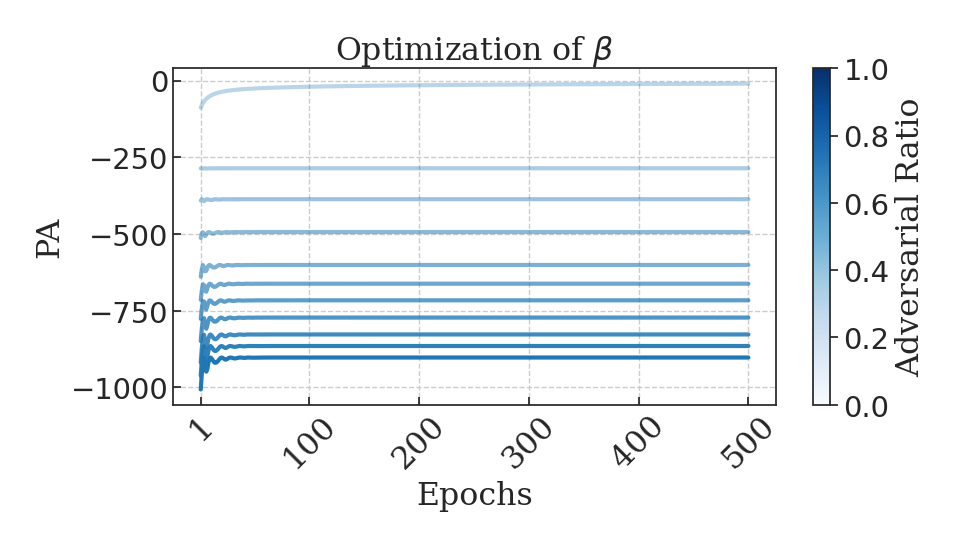
\includegraphics[width=\textwidth]{img/results_discussion/empirical/logpas.png}
    \end{subfigure}
    \caption{PA kernel optimization in the CIFAR10 gaussian noise setting for different ratio
    of perturbed samples. Perturbation magnitude is $\ell_\infty$ = 32 / 255.}
    \label{fig:gaussian_optimization}
\end{figure}

As expected, $\beta$ tends to infinity in the unperturbed case, and converges
quickly to its optimal value in the rest of cases, even if the sample size is considerably
large and memory-intensive. The decay in the PA value is less pronounced the higher
fraction of perturbed samples are there, as we observed in the artificial setting, which
is consistent with the concept of robustness itself, as it already approaches
the lower bound for these kinds of perturbation even when the whole sample has yet not
been perturbed. \\

\section{Adversarial setting}\label{sec:results_adversarial}

The first scenario in which covariate shift robustness will be tested is the
adversarial setting. This setting serves as an archetypal 
use case for any robustness metric, given that adversarial perturbations are
deliberately generated to mislead the model. By definition, the higher the
effectiveness of the attack, the lower the robustness score of the model. In particular, 
PA should be highly informative about the defensive capabilities of the model, as the posterior 
distribution over the hypothesis class will shift significantly in the 
presence of adversarial perturbations. This section aims to validate 
this claim and provide deeper insights into the nature of the metric. \\

It is important to note that adversarial perturbations constitute an
intermediate setting between sampling randomness and distribution shift. 
On the one hand, they emulate a sampling variation that appears 
as an outlier under the model's representation of the true class, even if
the source of variability is completely artificial. On the other
hand, samples are known to contain the set of features that should 
align with the inductive bias of the model, and so the model's ability to 
distillate those features is in question. In practice, we are evaluating the 
quality of the complex discriminator function defining a basin of stability
around original samples, and for that no deep understanding of the nature of 
the randomness of the samples or the features they encode is needed.\\

This interpretation is aligned with the measure provided by accuracy-based metrics, 
because adversarial samples are not expected to contain any relevant features of other
classes or express any accountable source of randomness, but instead exploit specific
vulnerabilities of models to specifically alter the position of the maximum of 
the posterior ditribution. A greater posterior overlap will still
indicate higher robustness to attacks, regardless of the nature of the model or the
attack, but optimal posteriors are expected to converge to very peaked gibbs
distributions centered at the predicted class, reducing the interpretability of PA
to that of accuracy. \\

In order to explore these claims, robustness and performance results will be
provided through the adversarial fidelity ratio (AFR) value and compared to those
yielded by PA. The AFR computed with the true class labels will be used as a baseline
of model performance, whereas the AFR computed with the predicted class label
will be a reference for robustness, as it aligns with the aforementioned
interpretation.

\begin{definition}[Adversarial fidelity ratio]
    Let $\bm{\hat{y}^\prime}, \bm{\hat{y}^{\prime\prime}} \in \mathcal{Y}^N$ be the predicted class 
    labels for $\bm{x}^\prime$ and $\bm{x}^{\prime \prime}$, respectively, 
    and $\bm{y}\in \mathcal{Y}^N$ the true labels. Let $\operatorname{ACC}$ be the standard accuracy 
    metric, as defined in Section \ref{sec:robustness_to_covariate_shift}.
    The adversarial fidelity ratio (AFR) is expressed as

    $$
    \begin{aligned}
        \operatorname{AFR (T)} &= \operatorname{ACC}(\bm{\hat{y}^{\prime \prime}}, \bm{y}), \\
        \operatorname{AFR (P)} &= \operatorname{ACC}(\bm{\hat{y}^{\prime \prime}}, \bm{\hat{y}^{\prime}}).
    \end{aligned}
    $$

\end{definition}

The results provided in this section have been obtained using the CIFAR10 dataset CITE1,
which is widely regarded as a standard benchmark for robustness evaluation. CIFAR10 is
a balanced dataset containing 60.000 coloured 32 $\times$ 32 pixel images belonging to 10
different classes. We will consider a pre-trained WideResNet-28-10 as a baseline, undefended
model and compare it to some state-of-the-art robust models provided by the 
RobustBench CITE2
library under PGD CITE3
and FMN CITE4
attacks, both run for a thousand steps (see Section \ref{sec:adversarial_setting}). 
The PGD attack power will be specified in terms of $\ell_\infty$, which corresponds
to the maximum perturbation allowed for each pixel. This is consistent with the characterization
of adversarial perturbation given in the previous chapter, as every perturbation will be bounded
to the region defined by $\mathbf{B}_\infty^{\ell_{\infty}} (x)$.

\begin{figure}[H]
    \centering
    \begin{subfigure}[b]{0.25\textwidth}
        \centering
        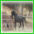
\includegraphics[width=\textwidth]{img/results_discussion/adversarial/adv_unperturbed_framed.png}
        \caption{Original}
    \end{subfigure}
    \hfill
    \begin{subfigure}[b]{0.25\textwidth}
        \centering
        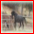
\includegraphics[width=\textwidth]{img/results_discussion/adversarial/adv_pgd_framed.png}
        \caption{PGD, $\ell_\infty$ = 36/255}
    \end{subfigure}
    \hfill
    \begin{subfigure}[b]{0.25\textwidth}
        \centering
        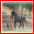
\includegraphics[width=\textwidth]{img/results_discussion/adversarial/adv_fmn_framed.png}
        \caption{FMN}
    \end{subfigure}
    \caption{Original and adversarially perturbed CIFAR10 sample. Both perturbations succeed
    at misleading an undefended pre-trained WideResNet-28-10 net.}
\end{figure}

Besides the maximum norm allowed for each perturbation, we are also interested in evaluating 
the sensitivity of our robustness measure to the ratio of perturbed samples in the dataset, 
also known as adversarial ratio (AR). The final adversarial dataset $\bm{x}''$ will be generated as

$$
\bm{x}'' := \operatorname{AR} \bm{x}'' + (1 - \operatorname{AR}) \bm{x}',
$$

where $\bm{x}'' = \bm{x}' + \bm{\Delta}$, as per Definition \ref{def:adversarial_perturbation}.
This incremental expansion of the attack is particularly relevant for PA, as we would initially 
expect it to behave non-linearly with respect to $\operatorname{AR}$ and converge faster to
the the $\operatorname{AR}=1$ robustness value than any accuracy-based metric, in light of the results obtained
in the previous section. We can quantify the model discriminability over increasing $\operatorname{AR}$
by computing the adversarial ratio gap $\Delta \operatorname{AR}$.\\

\begin{definition}[Adversarial ratio gap]
    Let $\gamma_+$ and $\gamma_-$ be two models, not necessarily different. Let $\operatorname{AR}_{+}$ and 
    $\operatorname{AR}_{-}$ be the adversarial ratio values such that

    $$
    \operatorname{PA}^{\gamma_+} \bigg|_{\operatorname{AR}_{+}} = \operatorname{PA}^{\gamma_-}\bigg|_{\operatorname{AR}_{-}}
    $$

    the aversarial ratio gap ($\Delta \operatorname{AR}$) is obtained as

    $$
    \Delta\operatorname{AR} = \operatorname{AR}_{+} - \operatorname{AR}_{-}. 
    $$
\end{definition}

Before delving into the results, it is worth exploring the immediate consequences
of the previous claim, namely the fact that the maximum posterior agreement will
be achieved when gibbs distributions are highly peaked on the predicted 
class, at least for moderately aggressive attacks. This is because most adversarial 
samples will not succeed at misleading the model and thus drive the inverse temperature to
infinity. The divergence of $\beta$ is only limited by the set of misleading adversarial 
samples, that for being perturbed from the original class are still expected to assign a
significant confidence to the original prediction, even if not the maximum anymore.
Table \ref{tab:entropy_gibbs} illustrates this claim by showing that $\beta^{*} > 1$ 
for all robust models, resulting in a substantial decrease of the entropy between initial and 
optimal posteriors. \\

\begin{table}[H]
    \centering
        \begin{tabular}{l|rr|rr}
        Defense & $\beta^{*}_{\text{PGD}}$ & $\Delta H_{\text{PGD}}$  & $\beta^{*}_{\text{FMN}}$ & $\Delta H_{\text{FMN}}$ \\
        \midrule
        {\color{tab:orange} \textbf{Undefended}} & 0.78 & 0.048 & 0.65 & 0.10\\
        {\color{tab:blue} \textbf{Engstrom et al.}} & 15.63 & -1.204 & 2.59 & -0.71\\
        {\color{tab:green} \textbf{Athalye et al.}} & 35.48 & -3.049 & 19.84 & -2.13 \\
        {\color{tab:red} \textbf{Wong et al.}} & 15.46 & -1.229 & 4.59 & -0.96\\
        {\color{tab:purple} \textbf{Addepalli et al.}} & 15.89 & -2.023 & 6.08 & -1.71 \\
        {\color{tab:brown} \textbf{Wang et al.}} & 11.24 & -1.833 & 2.53 & -1.41\\
        \bottomrule
        \end{tabular}
        \caption{
        Entropy difference $\Delta H = H(\beta^{*}) - H(\beta)$ in bits 
        for different models, obtained for FMN and $\ell_\infty$=8/255 
        PGD attacks, both at $\operatorname{AR} = 1$. Entropy values are 
        estimated using the average posterior distribution over correctly classified
        samples, which constitute the largest proportion of the dataset.
        Figures \ref{fig:pgd_distributions_undefended}-\ref{fig:pgd_distributions_bpda}
        show the initial and optimal average posteriors from which these values
        were computed.
        }
        \label{tab:entropy_gibbs}
\end{table}

This realization allows us to break down the dataset into subsets of observations
that contribute to the final PA value in different ways, and therefore improve
the interpretation of the resulting robustness measurement.
For a start, a robust model should be expected to correctly classify most of the 
original samples with high confidence, as they
contain the discriminative features that define each class. Also in the original 
dataset, lack of generalization to sampling randomness should be penalized, as confidence in
the predicted class is lowered. Regarding adversarial samples, a clear
distinction between robust and non-robust models should be made based on the success 
rate of perturbations and the confidence attributed to misleading predictions. Adversarial 
perturbations on samples originally misclassified will not be of much interest,
as the effect on prediction confidence should not be as significant as in
the correctly classified ones. An interpretable expression for PA in the adversarial
setting can be obained by approximating the optimal posterior for each of these
groups of observations. \\

\begin{theorem}[Approximated PA in the adversarial setting]
    Let $\Xi_{\text{ERR}}$, $\Xi_{\text{MIS}}$ and $\Xi_{\text{ADV}}$ be the approximated robustness
    contributions of correctly classified original samples, misclassified original samples,
    and misleading adversarial samples, respectively. Then, we can express

    $$
    \operatorname{PA} \approx \Xi_{\text{ERR}} + \Xi_{\text{MIS}} + \Xi_{\text{ADV}}
    $$

    where
    $$
    \begin{aligned}
        &\Xi_{\text{ERR}} = N \tau \rho \log \left( 1 - 2\delta_{\text{ERR}} \right), \\
        &\Xi_{\text{MIS}} = N (1- \tau) \rho \log \left( 1 - 2\delta_{\text{MIS}} \right), \\
        &\Xi_{\text{ADV}} = N \tau (1 - \rho) \log \delta_{\text{ADV}},
    \end{aligned}
    $$

    where $\tau$ is the accuracy of the model in the original data and $\rho \equiv$ AFR (P).
    Variables $\delta_{\text{ERR}}$, $\delta_{\text{MIS}}$ and $\delta_{\text{ADV}}$ account for the 
    average probability assigned to
    classes other than the predicted class for the three aforementioned cases 
    (see illustration in Figure \ref{fig:appendix_adv_illustration}).
    \label{thm:approximated_pa}
\end{theorem}
\begin{proof}
    See Apendix \ref{sec:appendix_results_adversarial}.
\end{proof}

Figures \ref{fig:appendix_adversarial_approx_pa_pgd} and \ref{fig:appendix_adversarial_approx_pa_fmn}
compare the true and approximated PA values under increasing adversarial ratio for
PGD and FMN attacks, respectively. It is clear that penalizations are overestimated, 
given that the average posterior probability was
used and differences by defect are more significant than those by excess due to
the nonlinear nature of the logarithm in the range $[0,1]$.
Besides, $\beta^{*}$ is fixed to its lowest possible value; that
is, when $\operatorname{AR} = 1$. This makes the approximation on the FMN attack less
reliable for smaller adversarial ratio settings, as $\beta^{*}$ decreases significantly
due to the effectiveness of the attack. \\

Nevertheless, the relative differences in the approximated PA values are consistent
with the true values, and the ranking of the models is largely preserved across different
adversarial ratios, especially for $\operatorname{AR} = 1$. For that reason, the
interpretability provided by the approximated PA expression will illustrate
the results, and will be used to better characterize the source of robust and unrobust behaviour
observed in the different models. \\


\subsection{Adversarial robustness assessment with PA}

The first results presented correspond to PGD attacks with different attack power 
$\ell_\infty$, namely 8/255, 16/255 and 32/255, for increasing ratio of 
perturbed samples in the CIFAR10 dataset.

\begin{figure}[H]
    \centering
    \begin{subfigure}[b]{\textwidth}
        \centering
        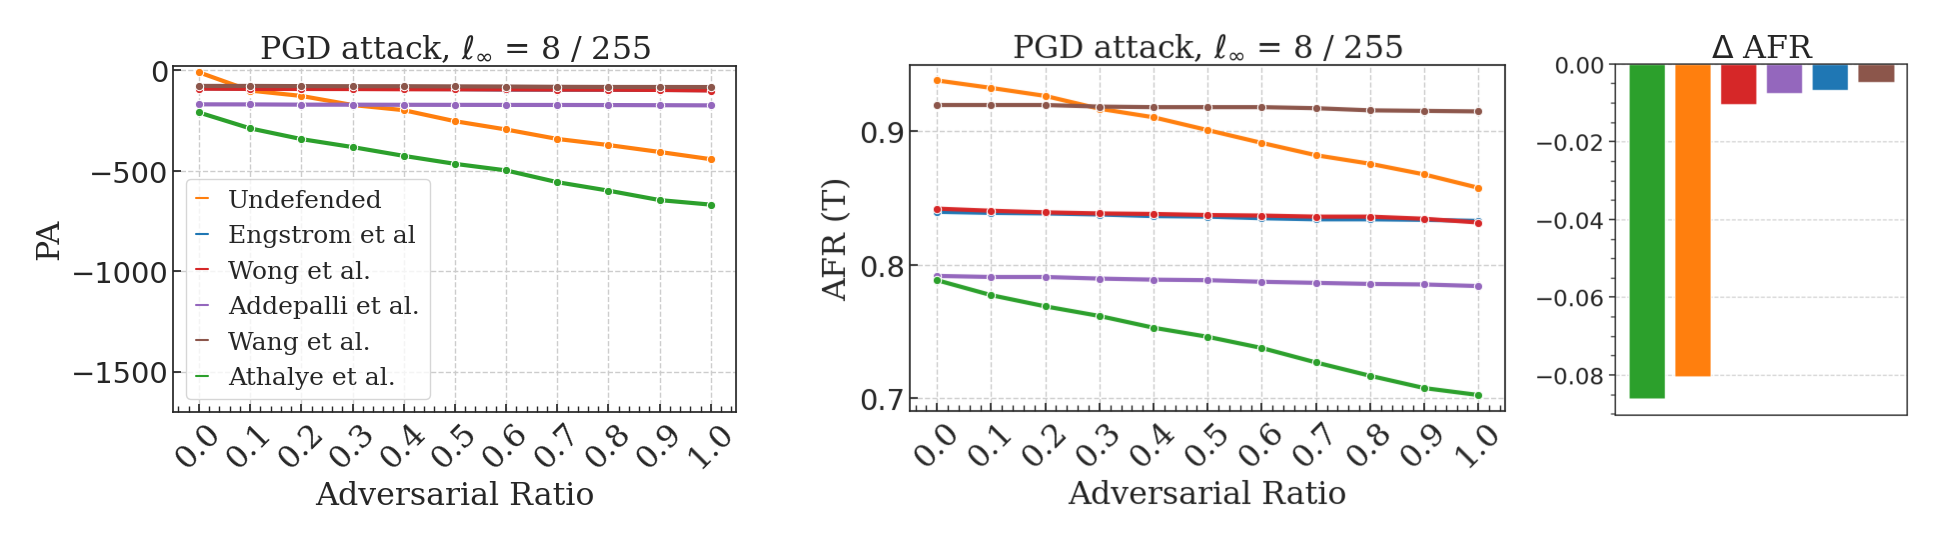
\includegraphics[width=\textwidth]{img/results_discussion/adversarial/PGD_0.0314_combo.png}
    \end{subfigure}

    \vspace{1em}

    \begin{subfigure}[b]{\textwidth}
        \centering
        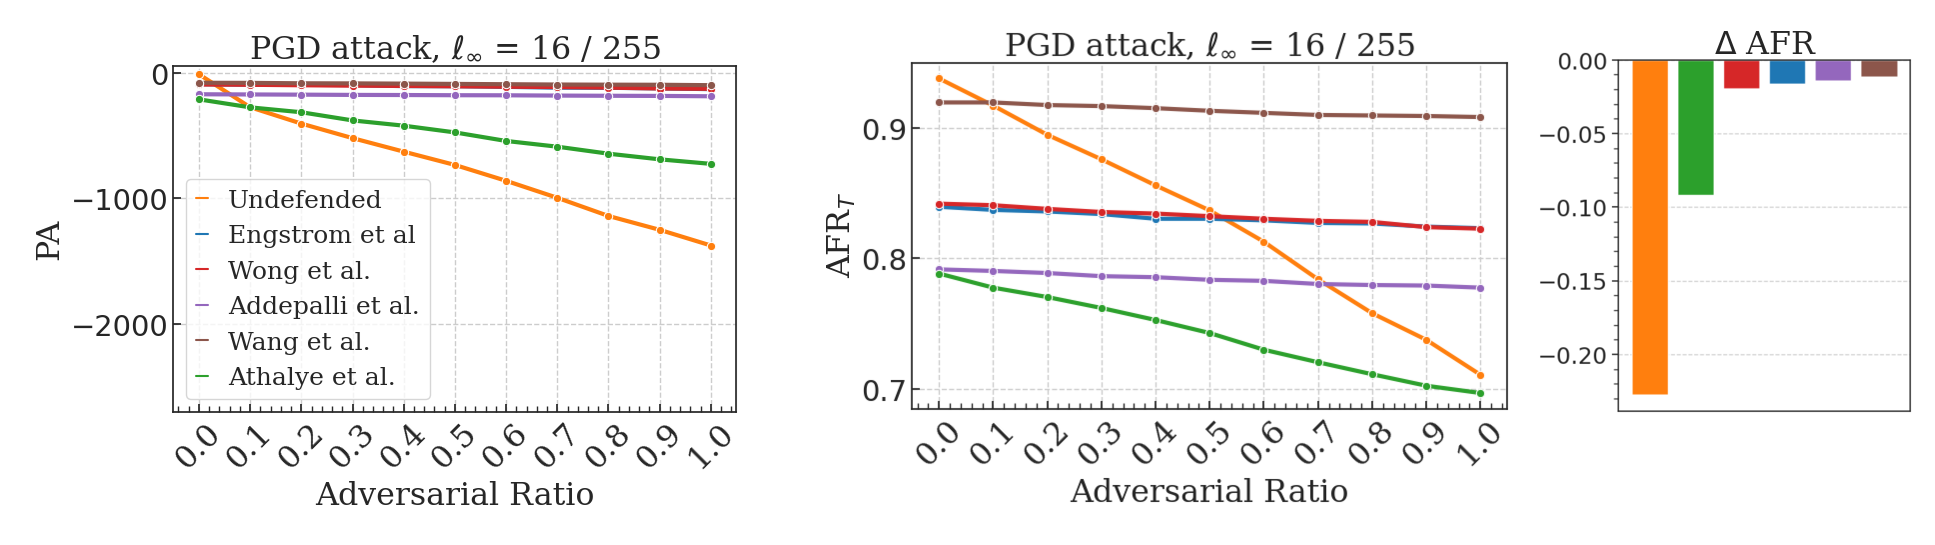
\includegraphics[width=\textwidth]{img/results_discussion/adversarial/PGD_0.0627_combo.png}
    \end{subfigure}

    \vspace{1em}

    \begin{subfigure}[b]{\textwidth}
        \centering
        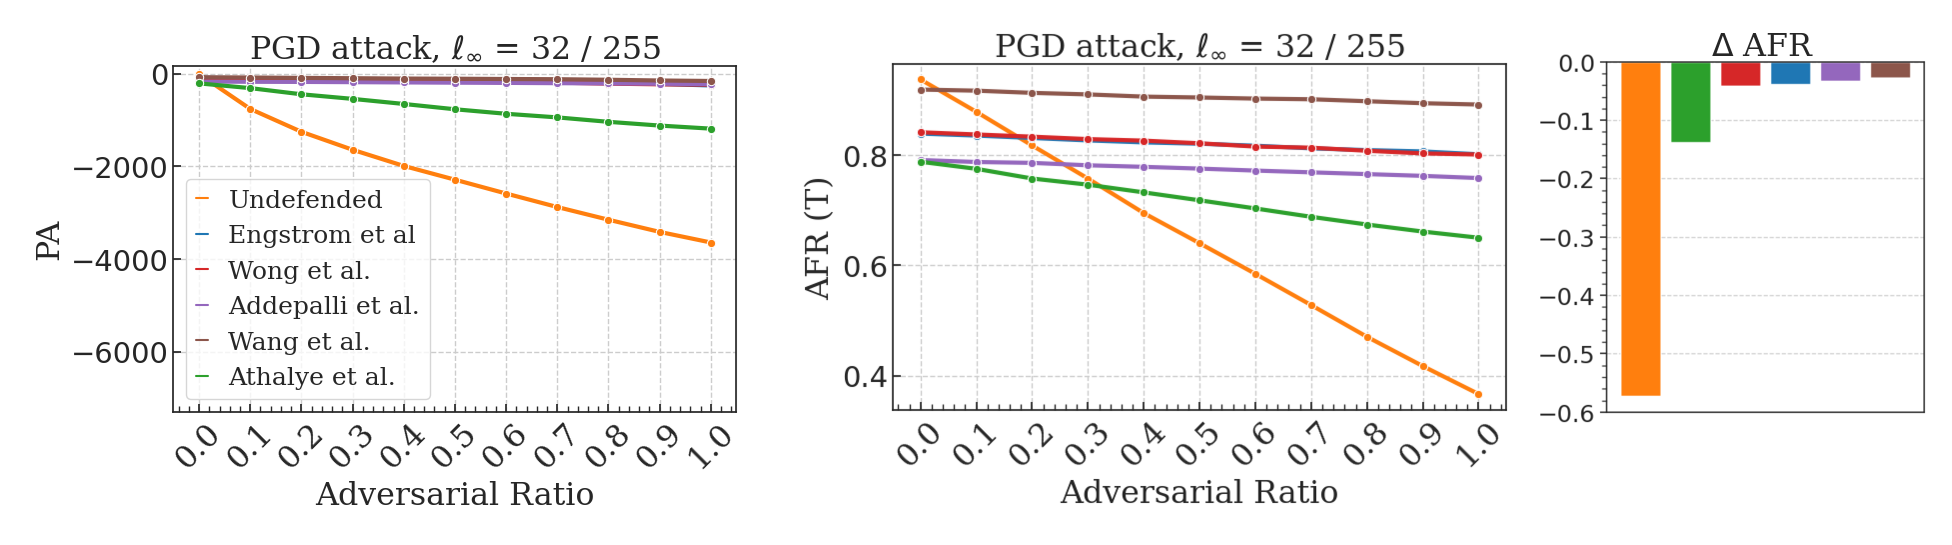
\includegraphics[width=\textwidth]{img/results_discussion/adversarial/PGD_0.1255_combo.png}
    \end{subfigure}

    \caption{PA, AFR(T) and the AFR variation against increasing adversarial ratio at different
    perturbation norm bounds. The aforementioned undefended net and several RobustBench
    robust models are considered under a 1000 step PGD attack.}
    \label{fig:six_figures_pa_adv}
\end{figure}

At first glance, it is clear that PA is able to discriminate robust models from
the {\color{tab:orange} \textbf{Undefended}} one, which is shown to significantly
decrease its performance with increasing adversarial ratio and attack power. As expected, 
the rate at which its performance decreases is higher
the more powerful the attack is, as a greater percentage of samples are able to
mislead its predictions. \\

From both PA and AFR stems the fact that {\color{tab:green} \textbf{Athalye et al.}}
is significantly less robust than its RobustBench counterparts to PGD attacks, since 
its performance decreases
way more significantly with increasing $\operatorname{AR}$. It is interesting to see, however,
than the rate at which its performance decreases is inversely proportional to the 
attack power, which indicates that the principle by which robustness is achieved
is more effective for large-norm perturbations. \\

A fundamental existing difference between these two models, that cannot be
inferred from a purely performance-based metric, is the nature of the shift in
the probabilistic output of the model, which is the source of the robust and non-robust
behaviour observed. Figure \ref{fig:unrobust_posterior_short_pgd} \textbf{(right)}
shows the optimal $\beta^{*}$ value for each model, which is an indication of
the entropy of the posterior distribution and discriminates the two non-robust
models from the rest and from each other. The {\color{tab:orange} \textbf{Undefended}}
model provides overconfident predictions that maximize disagreement in misleading and 
misclassified samples, whereas {\color{tab:green} \textbf{Athalye et al.}} provides 
uncertain predictions that minimize disagreement in adversarial samples but have 
the opposite effect in correctly classified ones. This insight clarifies the 
unintuitive behaviour observed earlier, by which {\color{tab:green} \textbf{Athalye et al.}} 
robustness value decreases at a lower rate with increasing attack power, despite maintaining a
constant decrease in performance of $\Delta \operatorname{AFR} \sim 0.1$. \\

Figure \ref{fig:unrobust_posterior_short_pgd} \textbf{(left)} illustrates
the previous reasoning by displaying the average posterior
probability assigned to the predicted class by each model, conditioned on the type
of response given by the model. This discrimination yields three groups of observations,
namely original samples that are correctly classified by the robust model, 
original samples that are misclassified and perturbed samples that, having their 
associated unperturbed sample been correctly classified, 
have been able to mislead the model. These three cases are relevant from the 
adversarial robustness perspective,  as they illustrate the trade-off between high-confident 
original predictions and adversarial vulnerability, which has been already stated in 
previous chapters. {\color{tab:brown} \textbf{Wang et al.}}
acts as a reference for an ideal robust behaviour, in which original samples are
predicted with high confidence and adversarially misleading predicted labels are 
only slightly more likely than the rest. Equivalent representations for the remaining
models can be found in Figure \ref{fig:appendix_adversarial_distribution_pgd}.\\

\begin{figure}[H]
    \centering
    \begin{subfigure}[b]{\textwidth}
        \centering
        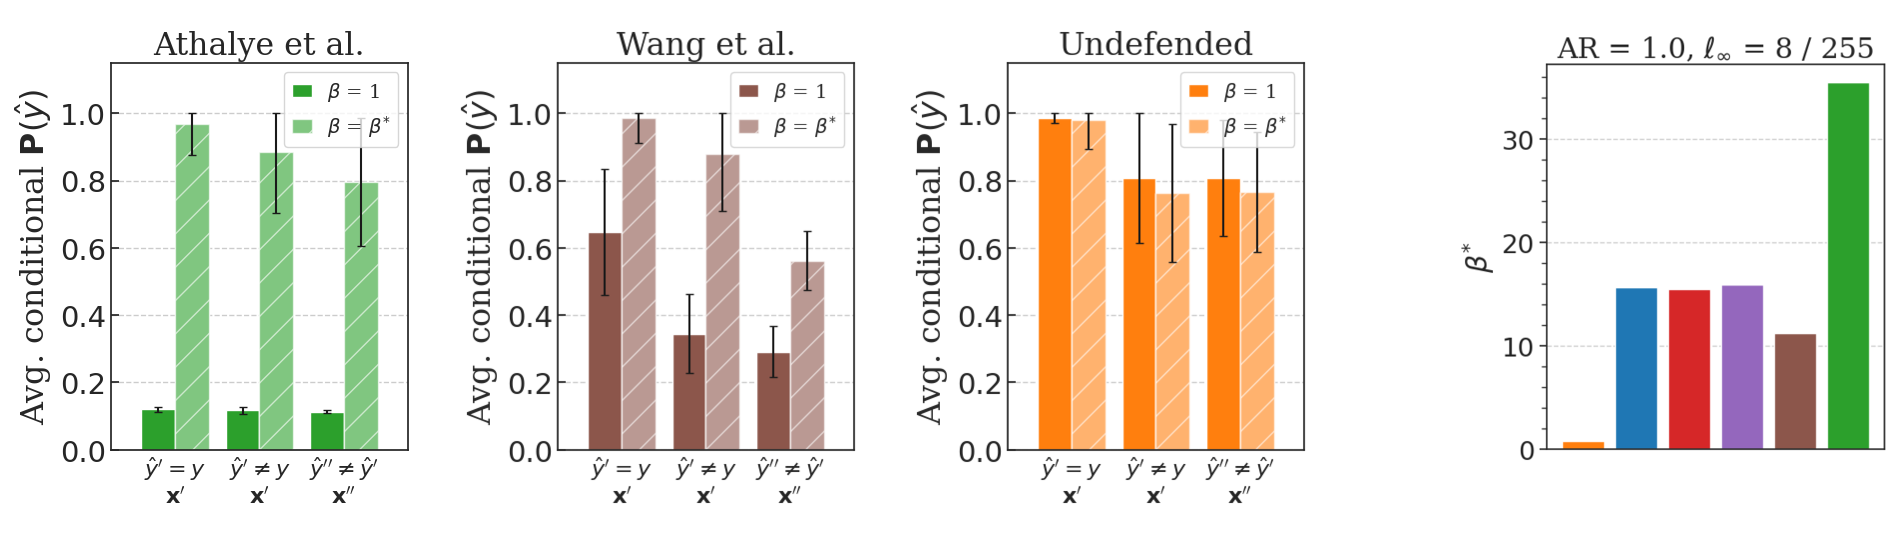
\includegraphics[width=\textwidth]{img/results_discussion/adversarial/bpda_wang_undefended_beta_pgd.png}
    \end{subfigure}
   
    \caption{(\textbf{left}) Average posterior probability of the predicted class for 
    correctly classified original samples, misclassified original samples, and 
    misleading adversarial samples, respectively. (\textbf{right}) Optimal $\beta^{*}$ value for each model.
    Results obtained through a PGD attack with $\ell_\infty = 8 / 255$.}
    \label{fig:unrobust_posterior_short_pgd}
\end{figure}

With respect to robust models, we observe a significant difference in the 
discriminative power of PA and accuracy-based metrics that does not immediately
derive from the informativeness of the optimal posterior. As remarked before, AFR (P)
constitutes our baseline robustness metric, as by definition represents the ratio
of predictions that remained constant under adversarial perturbations, and
therefore ranks models by their predictive capabilities against these attacks. The
value of $\Delta$AFR aligns with that definition, and discriminates robust models
by a very thin margin, selecting {\color{tab:brown} \textbf{Wang et al.}} as
the best. Further analysis on PA is needed to understand the source of this 
discrepancy, as for instance why {\color{tab:purple} \textbf{Addepalli et al.}} model
is attributed a significantly lower value than the remaining robust models
under a $\ell_\infty$=8/255 PGD attack, despite displaying a similar decrease in performance. \\

\begin{figure}[H]
    \centering
    \begin{subfigure}[b]{0.37\textwidth}
        \centering
        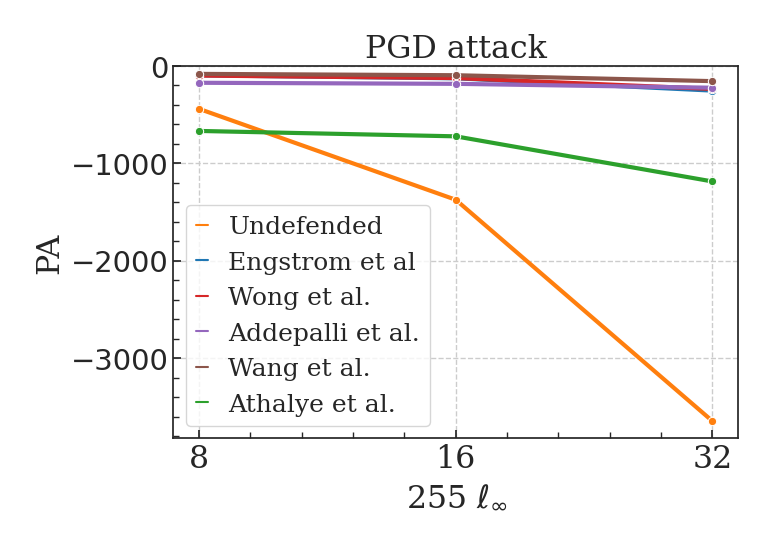
\includegraphics[width=\textwidth]{img/results_discussion/adversarial/PGD_logPA_eps.png}
    \end{subfigure}
    \hfill
    \begin{subfigure}[b]{0.59\textwidth}
        \centering
        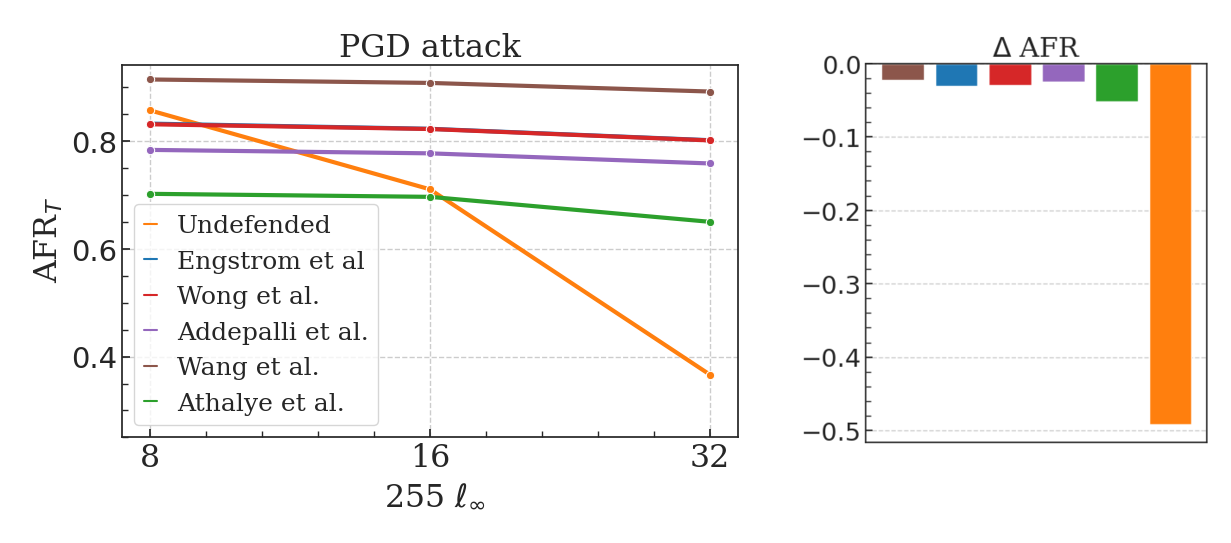
\includegraphics[width=\textwidth]{img/results_discussion/adversarial/PGD_AFR_true_eps_diff.png}
    \end{subfigure}
    \caption{PA, AFR(T) and the AFR variation against increasing attack power for  $\operatorname{AR} = 1$. 
    The aforementioned undefended net and several RobustBench robust models are considered
    under a 1000 step PGD attack.}
    \label{fig:pgd_eps}
\end{figure}

Finally, Figure \ref{fig:pgd_eps} shows that PA is also discriminative with respect to
increasing attack power, expressed through the maximum allowed $\ell_\infty$ norm. 
As mentioned earlier, PA values are heavily aligned with the performance
decrease of the models under a specific attack power, but the observed decrease in PA 
under increasing $\ell_\infty$ is much more significant that the decrease 
in performance. This can be explained by the fact that the metric is sensitive 
to the overall posterior shift and not only the position of the maximum. When increasing 
the attack power, confidence in the predicted class will decrease in general, 
even when the sample does not succeed at misleading the model, and therefore the
overall overlap between posteriors will be reduced even at comparable performance levels. \\

In order to widen the scope of the analysis, analogous results will be obtained for
a FMN attack, which is expected to be more effective than a PGD attack under 
the same conditions, given the overall decrease in $\beta^{*}$ observed 
in Table \ref{tab:entropy_gibbs}.
Figure \ref{fig:adv_fmn_pa_afr} shows the evolution of PA against 
increasing adversarial ratio for the same models, and compares
it with the assessment provided by AFR.


\begin{figure}[H]
    \centering
    \begin{subfigure}[b]{0.39\textwidth}
        \centering
        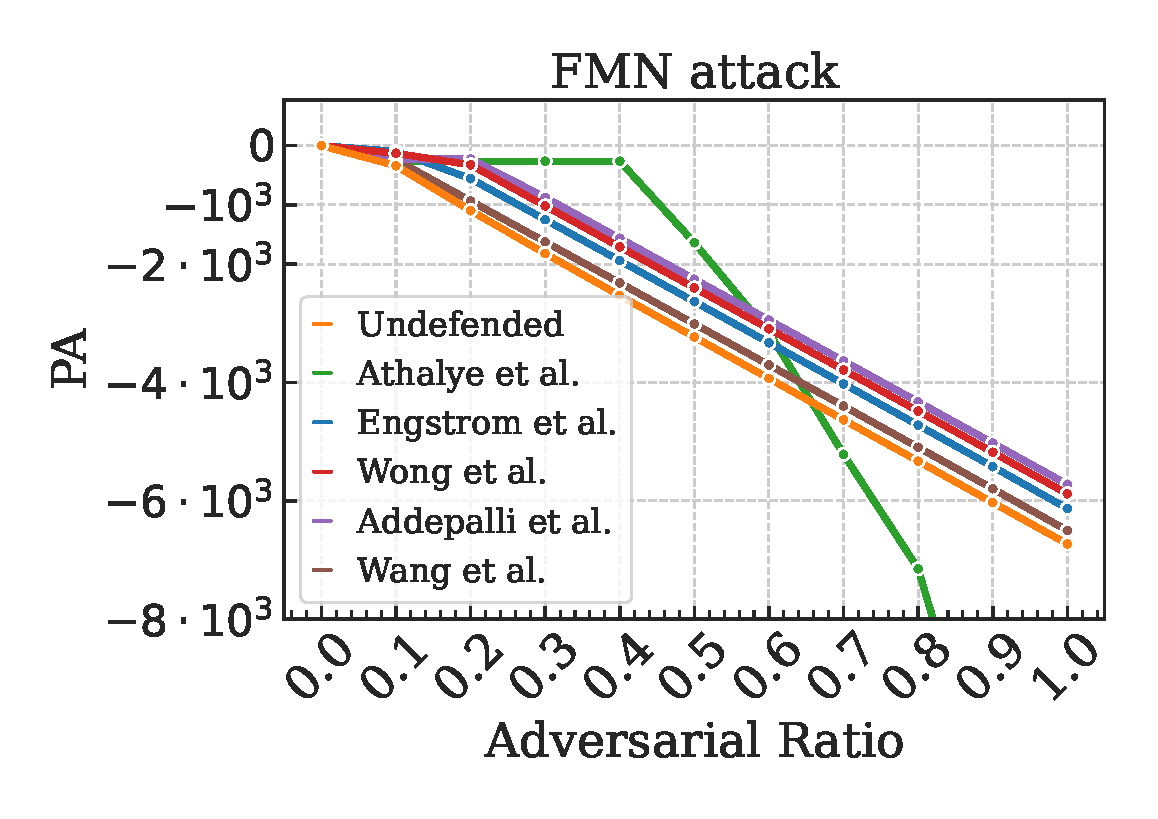
\includegraphics[width=\textwidth]{img/results_discussion/adversarial/FMN.pdf}
    \end{subfigure}
    \hfill
    \begin{subfigure}[b]{0.59\textwidth}
        \centering
        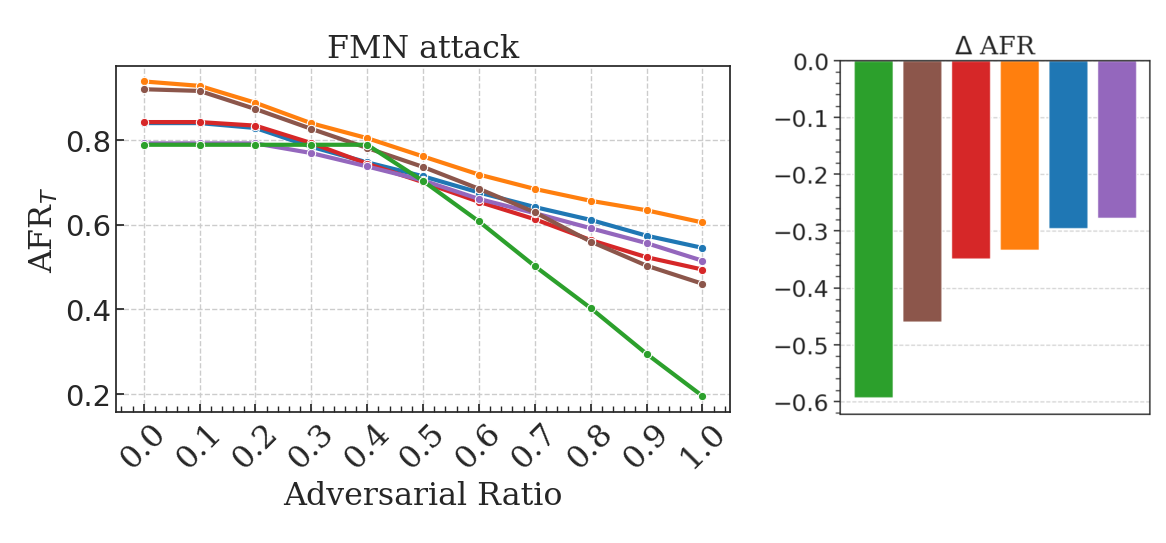
\includegraphics[width=\textwidth]{img/results_discussion/adversarial/FMN_1000_AFR_true.png}
    \end{subfigure}
    \caption{PA, AFR(T) and the AFR variation against increasing adversarial ratio. 
    The aforementioned undefended net and several RobustBench robust models are considered 
    under a 1000 step FMN attack.}
    \label{fig:adv_fmn_pa_afr}
\end{figure}


As expected, the effectiveness of the FMN attack is superior to that of PGD attacks, as
the decrease in performance is substantially more significant for all models, especially the ones
previously considered robust. It is likely that these models have been defended with a
compression strategy that succeeds at filtering out small perturbations, which are
the ones employed by FMN, and for that reason maintain their performance at low
adversarial ratio values CITE 5.
In particular, {\color{tab:green} \textbf{Athalye et al.}} remains maximally robust
until at least 40\% of the samples are perturbed, at which point the defensive strategy
is neutralized and a constant fraction of the additional perturbed samples succeeds at
misleading the model, which translates into a linear decrease in performance and PA. \\

PA proves to be very discriminative among robust models and to represent the 
phase transition entailed by the collapse of the defense strategy better than AFR does, which can be
observed in more detail in Figure \ref{fig:appendix_adversarial_afrpred_fmn}. A significative
result is that PA is not so directly aligned with $\Delta$AFR, in contrast to
the PGD case, which shows again that the decrease in performance is not the main driver of
the robustness assessment provided by PA, but instead can be interpreted as a consequence of
a misalignment in the posterior distributions of adversarial samples, which are the ones driving
the metric after the $\operatorname{AR}$ thresold is reached. \\

\begin{figure}[H]
    \centering
    \begin{subfigure}[b]{\textwidth}
        \centering
        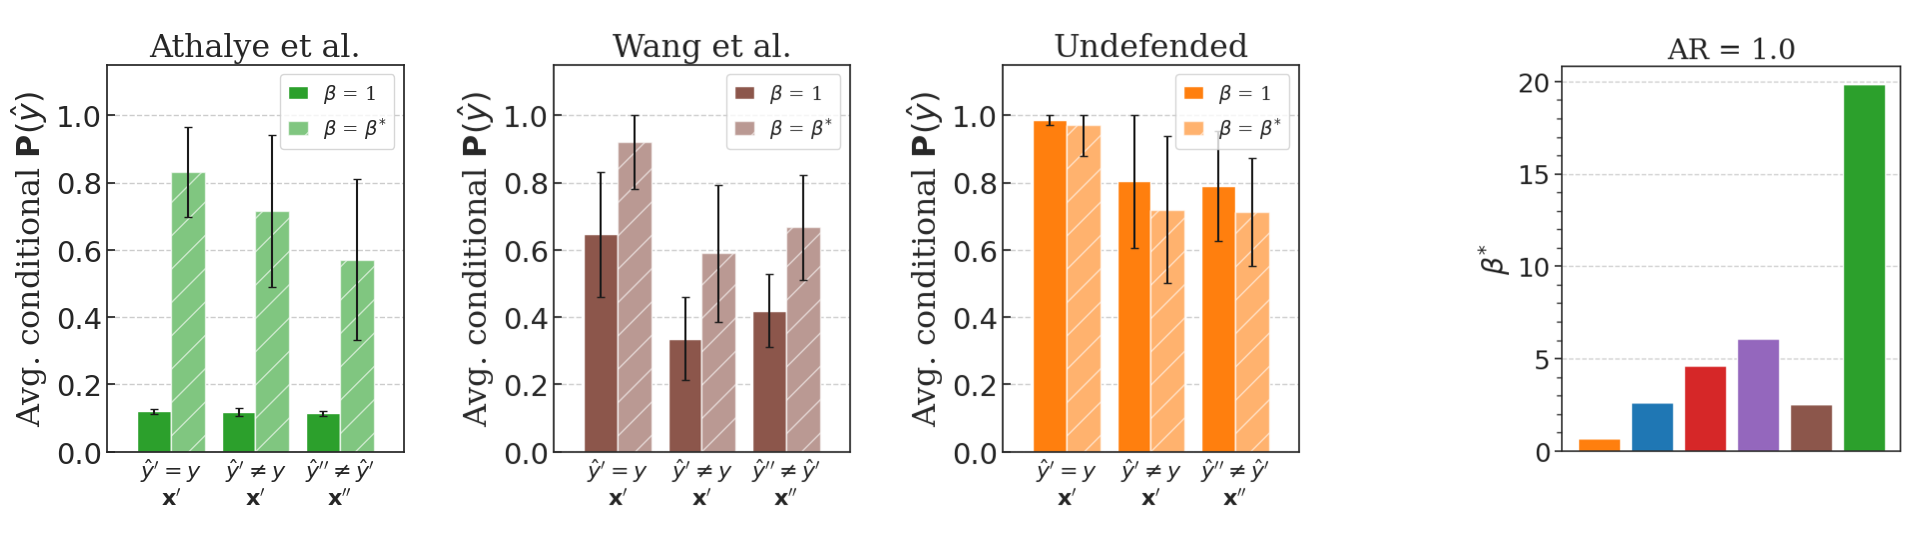
\includegraphics[width=\textwidth]{img/results_discussion/adversarial/bpda_wang_undefended_beta_fmn.png}
    \end{subfigure}
   
    \caption{(\textbf{left}) Average posterior probability of the predicted class for 
    correctly classified original samples, misclassified original samples, and 
    misleading adversarial samples, respectively. (\textbf{right}) Optimal $\beta^{*}$ value for each model.
    Results obtained through a FMN attack.}
    \label{fig:unrobust_posterior_short_fmn}
\end{figure}

Figure \ref{fig:unrobust_posterior_short_fmn} gives insight into the probabilistic output
of the model and the informativeness of the optimal posterior for the {\color{tab:orange} \textbf{Undefended}}, 
{\color{tab:green} \textbf{Athalye et al.}} and {\color{tab:brown} \textbf{Wang et al.}} models, in
analogous way to the PGD experiments. The first two models display a very similar behaviour for 
$\beta = 1$, but optimal posteriors are less informative due to the increased number of misleading
samples, which translates into a smaller $\beta^{*}$. The response of 
the {\color{tab:brown} \textbf{Wang et al.}} model further illustrates the higher effectiveness of
FMN attacks, as adversarial perturbations are on average more misleading than outlier samples in
the original dataset, which did not occur in the PGD case. Analogous representations for the remaining
models can be found in Figure \ref{fig:appendix_adversarial_distribution_fmn}, which show
that the {\color{tab:purple} \textbf{Addepalli et al.}} is the only robust model that maintains
the same behaviour under both attacks.\\

Overall, we recognize that PA has a higher discriminative power than AFR, especially
considering the evolution of each metric over increasing adversarial ratio, as
seen in Figures \ref{fig:six_figures_pa_adv} and \ref{fig:adv_fmn_pa_afr}. 
In particular, Figures \ref{fig:appendix_adversarial_afrpred_pgd} and \ref{fig:appendix_adversarial_afrpred_fmn}
compare the evolution of PA with that of AFR (P), which is the baseline metric for robustness,
and show the susceptibility of the latter to dataset variability. This is an important
consideration, as PA not only improves the discriminability in terms of the scale of
the differences between models, but also provides a more stable assessment across varying
levels of perturbed sample presence, under which AFR (P) exhibits significant fluctuations
that alter the ranking of the models at every step. \\

These observations lead to the conclusion that PA offers a more reliable
assessment of adversarial robustness, which in general aligns with the decrease
in performance on perturbed samples, but that relies heavily on the informativeness
of the posterior distribution and the confidence in the predictions for both
original and perturbed samples. \\

\subsection{Interpretability of PA in the adversarial setting}

In light of the results obtained, the suitability of
PA in the adversarial setting has been demonstrated, but a deeper exploration of the
reason of the discrepancies between PA and the baseline robustness measures is needed
so that it can confidently be established as a model selection criterion. In particular,
we will work with the approximated expression of PA derived in Theorem \ref{thm:approximated_pa} 
and ellucidate the source of the measured robust behaviour.

Table \ref{tab:approx_pa_pgd_table} shows the contribution of each subset of observations to the final
approximated PA value for a PGD attack. $N_{\text{ERR}}$, $N_{\text{MIS}}$ and $N_{\text{ADV}}$ are the number of (pairs of)
contributing samples, and $\Xi_{\text{ERR}}$, $\Xi_{\text{MIS}}$ and $\Xi_{\text{ADV}}$ are
the total amount of the contribution. For reasons described earlier in this section,
the PA approximation overestimates penalizations when compared to the true value, but
relative discrepancies between models are still largely preserved and therefore the rationale
behind the discriminative power of PA, as shown in Figures \ref{fig:appendix_adversarial_approx_pa_pgd}
and \ref{fig:appendix_adversarial_approx_pa_fmn}. The parameters $2 \delta_{\text{MIS}}$ and
$\delta_{\text{ADV}}$ account for the average probability assigned to classes other than the predicted
class for misclassified original samples and misleading adversarial samples, respectively, and 
help interpret the informativeness of the distibution as well as the value of each individual 
penalization. \\

For instance, a large $2 \delta_{\text{MIS}}$ value indicates robustness to sampling randomness, as it
represents higher average uncertainty in misclassified predictions. A model with a high performance on 
test data entails a more negative penalization $\log(1 - 2 \delta_{\text{MIS}})$, for being misclassified 
samples more likely to be equivalently misclassified under adversarial perturbations, but at
the same time makes misclassifications less likely, and therefore the number of terms added to
$\Xi_{\text{MIS}}$. The existing trade-off between standard and robust generalization arises when 
following this reasoning towards the minimization of $\Xi_{\text{MIS}}$, because reducing the number of 
misclassified samples will drive $\beta^{*}$ to higher values and therefore decrease adversarial 
uncertainty $\delta_{\text{ADV}}$. As outlined before, $\delta_{\text{ADV}}$ indicates 
robustness to adversarial perturbations, as it represents the average prediction uncertainty on adversarial 
misleading samples, and entails a penalization of $\log(\delta_{\text{ADV}})$. \\

The interpretation of these terms is vitally important for the purpose of this work, as it enables
the identification of the different sources of robustness displayed by each model, and therefore
the characterization of the randomness that we will demand models to generalize to. From a general 
perspective, $\Xi_{\text{ERR}} + \Xi_{\text{MIS}}$ can be understood as the lack of robustness
to sampling randomness, and $\Xi_{\text{ADV}}$ as the lack of robustness to adversarial perturbations. \\

\begin{table}[H]
    \centering
    \begin{tabular}{l|rr|rrr|rrr}
    Defense & $N_{\text{ERR}}$ & $\Xi_{\text{ERR}}$ & $N_{\text{MIS}}$ & $2 \delta_{\text{MIS}}$ & $\Xi_{\text{MIS}}$ & $N_{\text{ADV}}$ & $\delta_{\text{ADV}}$ & $\Xi_{\text{ADV}}$ \\
    \midrule
    {\color{tab:brown} \textbf{Wang et al.}} & 9148  & -248.38 & 799 & 0.24 & -220.24 & 47 & 0.44 & -39.44 \\
    {\color{tab:blue} \textbf{Engstrom et al.}} & 8328  & -273.26 & 1591 & 0.17 & -293.46 & 67 & 0.39 & -63.43 \\
    {\color{tab:red} \textbf{Wong et al.}} & 8329  & -254.37 & 1562 & 0.17 & -282.88 & 90 & 0.38 & -88.98 \\
    {\color{tab:purple} \textbf{Addepalli et al.}} & 7840  & -390.25 & 2063 & 0.21 & -487.17 & 75 & 0.46 & -58.92 \\
    {\color{tab:orange} \textbf{Undefended}} & 8569  & -372.49 & 566 & 0.47 & -364.14 & 810 & 0.24 & -1173.55 \\
    {\color{tab:green} \textbf{Athalye et al.}} & 7136 & -458.39 & 1915 & 0.23 & -505.46 & 747 & 0.21 & -1183.96 \\
    \bottomrule
    \end{tabular}
    \caption{
    Approximated PA contributions for a PGD attack with $\ell_\infty$ = 8/255 and 
    $\operatorname{AR} = 1.0$. The number of contributing samples for each term is 
    $N_{\text{ERR}} = \lfloor N \tau \rho \rfloor$, $N_{\text{MIS}} = \lfloor N (1-\tau) \rho \rfloor$ and
    $N_{\text{ADV}} = \lfloor N \tau (1-\rho) \rfloor$. The penalization argument $2 \delta_{\text{ERR}}$ has not
    been included for being negligible in all cases.
    }
    \label{tab:approx_pa_pgd_table}
\end{table}

- $\Xi_{\text{ERR}}$ aligns perfectly with AFR(T) at AR=1, given that penalization terms are 
similar for being beta quite high.\\
- $\Xi_{\text{MIS}}$ adds to this penalization but in a much more non-linear way, and illustrate
the trade-off described before, by which models containing less correct observations have smaller
penalization terms (larger dmis, see athalye), but more samples contributing, which adds up
to a higher total penalization. In the absence of adversarial samples, these models would be the most
robust. Undefended > Addepalli > Athalye.\\

- $\Xi_{\text{ADV}}$ is the least discriminative term, which makes sense given the small effectivity
of the attack. The $\Xi_{\text{ADV}}$ is driven by the decrease in performance beacuse its the number
of terms Nadv, but its modulated by the penalization term derived from dadv. This amounts to
the general interpretation of the PA kernel, which is equivalent to accuracy but instead of adding 
binary penalizations it contributes with a negative penalization term in the range [-inty, 0].\\

THIS SHOULD BE IN THE END.
- When we sum these contributions, we lose the direct dependency on AFR(T) and Delta AFR, because
we aggregate the robustness penalization contributed by the two sources of robustness. \\
This is a very important realization, as we show that PA provides a unified approach to robust model
selection, that unifies sampling randomness and adversarial randomness into a single
value. A weighted metric between AFR(T) and DeltaAFR (or AFR (T)) would be completely arbitrary
and would not adjust to the particularities of each model output. For instance, Undefended should be
penalized for its lack of robustness to adversarial examples, whereas Athalye should be penalized
for its lack of robustness to adversarial perturbations. PA provides a unified way of doing that
based on the whole probability distribution and therefore 


The values displayed on the tables cannot be compared in between attacks, as they are tied
to a specific value of $\beta^{*}$. 

\begin{table}[h]
    \centering
    \begin{tabular}{l|rr|rrr|rrr}
    Defense & $N_{\text{ERR}}$ & $\Xi_{\text{ERR}}$ & $N_{\text{MIS}}$ & $2 \delta_{\text{MIS}}$ & $\Xi_{\text{MIS}}$ & $N_{\text{ADV}}$ & $\delta_{\text{ADV}}$ & $\Xi_{\text{ADV}}$ \\
    \midrule
    {\color{tab:purple} \textbf{Addepalli et al.}} & 2864 & -401.85 & 753 & 0.52 & -553.50 & 1093 & 0.28 & -1394.45 \\
    {\color{tab:orange} \textbf{Undefended}} & 3123 & -182.56 & 206 & 0.56 & -169.73 & 1566 & 0.29 & -1953.27 \\
    {\color{tab:red} \textbf{Wong et al.}} & 2749 & -243.81 & 516 & 0.46 & -318.95 & 1460 & 0.27 & -1922.20 \\
    {\color{tab:blue} \textbf{Engstrom et al.}} & 2945 & -525.45 & 562 & 0.72 & -709.37 & 1252 & 0.32 & -1424.00 \\
    {\color{tab:brown} \textbf{Wang et al.}} & 2490 & -424.24 & 217 & 0.82 & -375.30 & 2107 & 0.33 & -2318.73 \\
    {\color{tab:green} \textbf{Athalye et al.}} & 1602 & -665.08 & 429 & 0.57 & -362.03 & 2339 & 0.43 & -1977.71 \\
    \bottomrule
    \end{tabular}
    \caption{
    Approximated PA contributions for a FMN attack with 
    $\operatorname{AR} = 1.0$. The number of contributing samples for each term is 
    $N_{\text{ERR}} = \lfloor N \tau \rho \rfloor$, $N_{\text{MIS}} = \lfloor N (1-\tau) \rho \rfloor$ and
    $N_{\text{ADV}} = \lfloor N \tau (1-\rho) \rfloor$. The penalization argument $2 \delta_{\text{ERR}}$ has not
    been included for being negligible in all cases, with the exception of {\color{tab:green} \textbf{Athalye et al.}}, in which 
    it amounts to $0.36$ and explains the large value of $\Xi_{\text{ERR}}$.
    }
    \label{tab:approx_pa_fmn_table}
\end{table}

This expression allows us to interpret the results of PA in the adversarial setting. For instance,
we expect a baseline PA value at $\operatorname{AR} = 0.0$q  driven by the accuracy of the model



Even if the ultimate 


Both models 
Given the shape of the posterior, mismatched samples will be
highly pena\\

AFTER THE PLOT OF THE TWO.

The ideal is to maximize confidence on true samples, keeping high accuracy, 
and minimize confidence in adversarial samples. If standard performance is significantly high,
then optimal beta will be lower the higher is the confidence in correctly classified original samples.
If, at the same time, the confidence in misleading samples is low, the gibbs posterior will be small
and therefore the penalization will be reduced. 

That's why PA behaves as an intermediate between a performance metric and a robustness metric,
in the sense that PA penalization terms will be lower the lower is the confidence in
adversarially misleading prediction, but at the same t

Given the non-linearity of the logarithm in
the interval $[0,1]$, the second option is b
optimal posterior for adversarial samples will not be very hig


\
 arises due to overfitting to the data, and results in a model that
not


This
results in a very low optimal $\beta$ value, as shown in Figure \ref{fig:unrobust_posterior_short} (\textbf{right}),




Both models show an opposite behaviour regarding their predictive outcome,

These results illustrate the prediction 



as per the robustness trade-off
mentioned in previous chapters, a

Once the source of discrimination between the {\color{tab:orange} \textbf{Undefended}} and
{\color{tab:green} \textbf{Athalye et al.}} models has been established, we can proceed 
with the exploration of the discrimination established between the {\color{tab:purple} \textbf{Addepalli et al.}}
model and the remaining robust models, which is maximum for $\ell_\infty = 8 / 255$ and
vanishes for $\ell_\infty = 32 / 255$. \\


WHEN YOU SHOW THE PLOTS: EXPLAIN THE REASON BEHIND LINEAR BEHAVIOUR, ETC...
(see ).

he value of $\Delta$ AFR aligns
with that of AFR(P), and obviously succeeds at discriminating 

$\Delta$ AFR is
the baseline robustness metric, as it represents t

as the model is not able to maintain its predictive

which in these experiments correspond to the  and 
{\color{tab:green} \textbf{Athalye et al.}} cases. This is clear from the fact that these
two models 


These results show that PA is consistently discriminating 

As we can see, PA consistently discriminates between the twho models over increasing
attack power.

- The undefended model shows the vulnerability of accuracy, because there is no regularization (defense) that makes a specific region in the latent space around the original sample that makes the model yield the same prediction. Even if the performance of the model is higher than that of robust models for low AR values, the Undefended model is clearly less robust, and only PA is able to account for that.
- The rest of the models only decrease slightly in performance with increasing shift ratio, because most of perturbed predictions yield the same result. In that sense, all models achieve similar levels of robustness. PA clearly distinguishes those two groups.

We would like to know where does this discrimination stem from, and for that we will have to dive deeper into the predictions yielded by the different models.


- To begin with, we can compare how does PA adjust to the actual measurement of robustness as per the classical definition in the adversarial setting. Looking at the results, we see that the principal driver of the discrimination in PA can be explained by the accuracy decrease between models. As expected, AFR (P) represents the classical definition of robustness, as its value is driven by the ratio of performance decrease.
- Some examples that we will consider:
    - Difference between the robust group vs the non-robust group (BPDA and Standard):
        - We can see that this distinction is made clear in both AFR and PA. Both models are less robust in 8/255 because their performance drops with increasing adversarial ratio, indicating that advesarial samples are able to mislead the model significantly. This distinction is seen more clearly in the optimal beta values, as BPDA and Undefended are clear outliers.
        - Posterior agreement discriminates models better, and aligns more with the expected linear decay of robustness over linear incremental adversarial ratio.
    - Difference between non-robust (BPDA and Standard)
        - At 8/255 we have almost same robustness, because accuracy slopes decrease at the same rate in AFR(T), and at 32/255 we have BPDA gains robustness. This is better seen in the DeltaAFR plot, as it represents the classical robustness metric **baseline**.
        - Both models are discriminated by the beta value, but we see that they are outliers in different directions. This indicates a fundamental difference in the robustness expression that will also be important to understand the discrimination made from Addepalli and the rest.
        - There is an intrinsic difference between distributions in the BPDA case and the Standard case. This is only distinguished by PA. First, because its evolution (decrease rate) is aligned with the observed robustness baseline. But also because the predictive behaviour of both models is intrinsically different, and that can only be seen using BETA. Maybe show the beta plot. CONSIDER ADDING THE BETA PLOT IN THE THEORY, AND THEN REFERENCE IT HERE.
            - [REFERENCE TO BETA PLOT]
- Regarding PA, we see nevertheless that the discriminative power is driven by something additional, that does not vary in between positive ARs for the robust models, and that allows us to discriminate Wang et al. (purple) from the other robust models when epsilon is small, and also BPDA from Standard for 8/255, even if both models present a similar decrease in performance.  In order to ellucidate that, we have to take a direct look to the model’s predictions.
    - [PLOT]: Relationship between prediction confidence and beta when AR=0.0. All three models have comparable performances, but their predictive output is completely different. This plot illustrates the meaning behind the value of optimal beta.


\begin{figure}[H]
    \centering
    \begin{subfigure}[b]{0.3\textwidth}
        \centering
        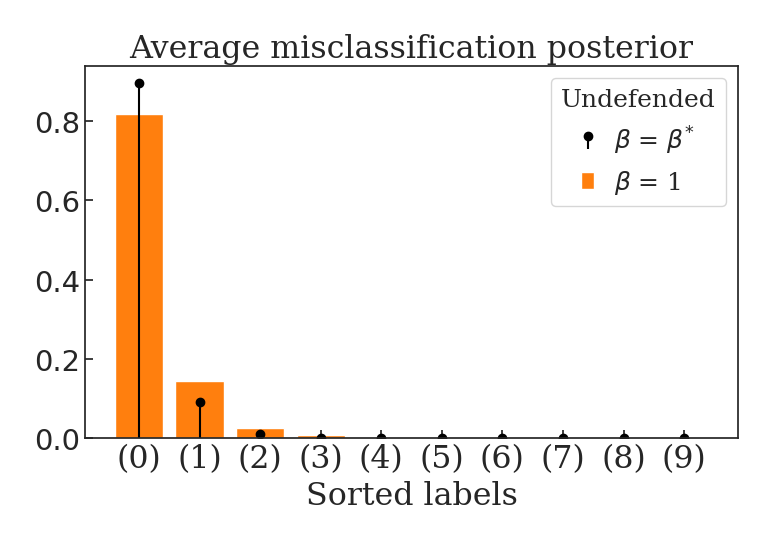
\includegraphics[width=\textwidth]{img/results_discussion/adversarial/PGD_0.0314_probability_misclass_standard.png}
    \end{subfigure}
    \hfill
    \begin{subfigure}[b]{0.3\textwidth}
        \centering
        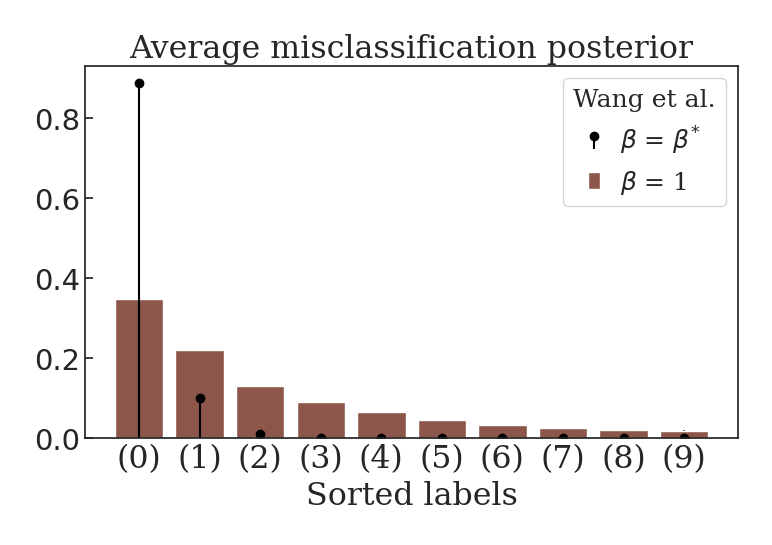
\includegraphics[width=\textwidth]{img/results_discussion/adversarial/PGD_0.0314_probability_misclass_wang2023.png}
    \end{subfigure}
    \hfill
    \begin{subfigure}[b]{0.3\textwidth}
        \centering
        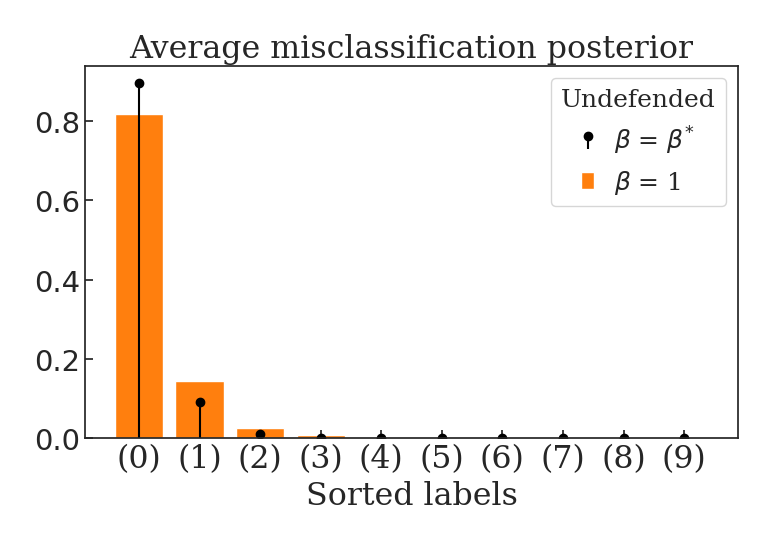
\includegraphics[width=\textwidth]{img/results_discussion/adversarial/PGD_0.0314_probability_misclass_standard.png}
    \end{subfigure}
    \caption{Relationship between prediction confidence and beta when AR=0.0. All three models have comparable performances, but their predictive output is completely different. This plot illustrates the meaning behind the value of optimal beta.}
\end{figure}

- It is worth noting that this is a 10-class classification problem, and we expect wrong predictions in the original dataset to have a more flattened distribution than correct predictions. For that reason, we expect PA to penalize disagreement over correct predictions than over incorrect predictions, and therefore to be more highly correlated with the true performance AFR (T) than with the actual robustness in the classical sense AFR (P). We can see this below.



AR=1.0. We can explain the posterior agreement values by looking at this plot, which represents the difference between the probability assigned to the highest confidence prediction for true, original samples and false, adversarial samples. As we can see, some models yield a higher confidence to the right class, nevertheless still yield high confidence to the wrong adversarial predicted class. Balance between low adversarial probability and wide gap between original true and adv false. ONLY ONE OF THEM IS ENOUGH

\begin{figure}[H]
    \centering
    \begin{subfigure}[b]{0.49\textwidth}
        \centering
        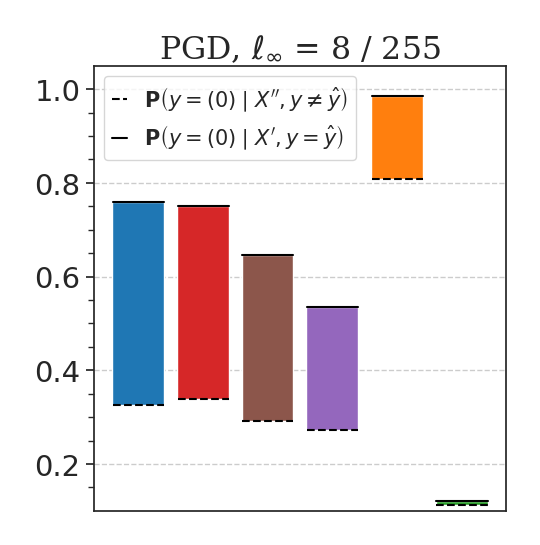
\includegraphics[width=\textwidth]{img/results_discussion/adversarial/DIFF_PGD_0.0314.png}
    \end{subfigure}
    \hfill
    \begin{subfigure}[b]{0.49\textwidth}
        \centering
        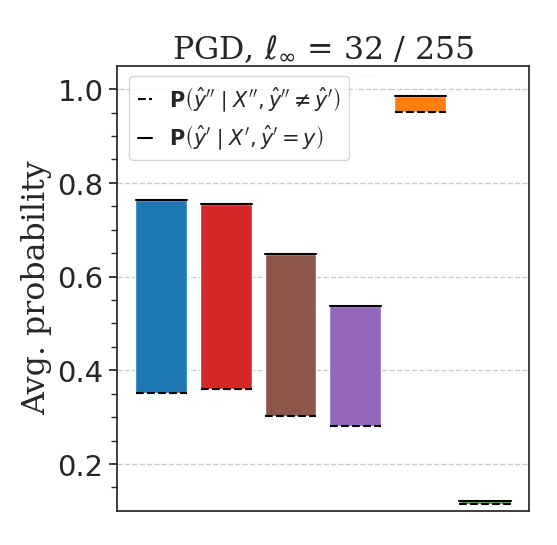
\includegraphics[width=\textwidth]{img/results_discussion/adversarial/DIFF_PGD_0.1255.png}
    \end{subfigure}
    \caption{Difference.}
    \label{fig:gaussian_optimization}
\end{figure}


Also works with FMN:
- Posterior agreement discriminates models in a different way as does AFR.
- Now we observe a great decrease of PA under increasing shift ratio.
- FMN is way more effective at decreasing accuracy.


- We can compare with PGD:
    - Original accuracy is the same because models are the same.
    - In all ROBUST models, FMN attacks are more successful because, on average, a higher confidence is given to adversarial misleading examples. The non-robust model behaves similarly, and the accuracy drop (see before) is also similar.
    - FMN attacks are more successful in RED than BLUE, as the accuracy drop is larger and the

\begin{figure}[H]
    \centering
    \begin{subfigure}[b]{0.49\textwidth}
        \centering
        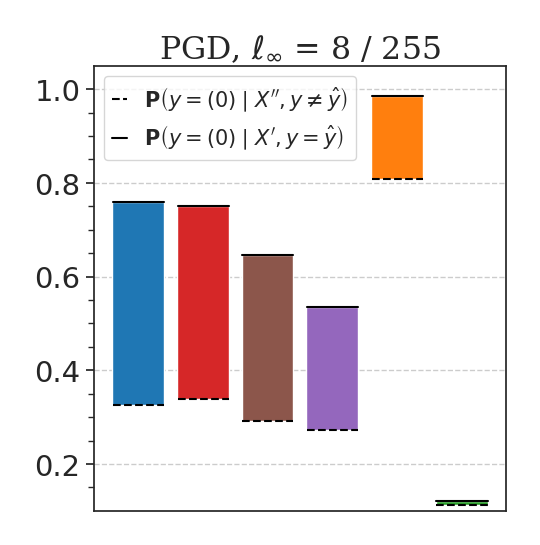
\includegraphics[width=\textwidth]{img/results_discussion/adversarial/DIFF_PGD_0.0314.png}
    \end{subfigure}
    \hfill
    \begin{subfigure}[b]{0.49\textwidth}
        \centering
        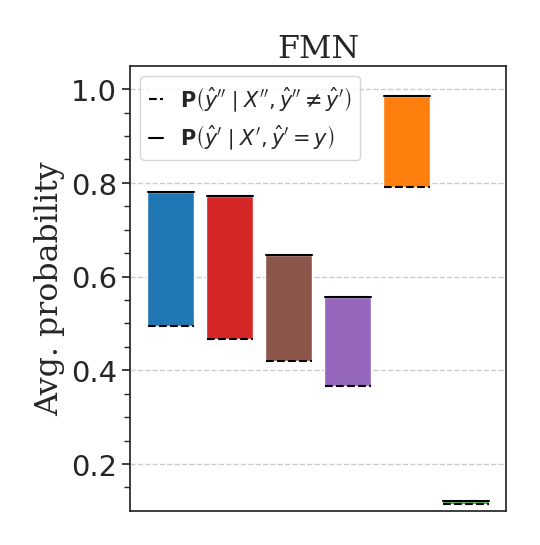
\includegraphics[width=\textwidth]{img/results_discussion/adversarial/DIFF_FMN.png}
    \end{subfigure}
    \caption{Difference.}
    \label{fig:gaussian_optimization}
\end{figure}


PROOF: Wasserstein and KL.

- An aggregated similarity measure between distributions is very informative but it does not correctly predict robustness in the outcome, as it treats all labels equally. This means that there is no penalization for disagreement or agreement, which is key for robustness assessment. For instance, BPDA is not penalized for having a flat distribution.

\begin{figure}[H]
    \centering
    \begin{subfigure}[b]{0.45\textwidth}
        \centering
        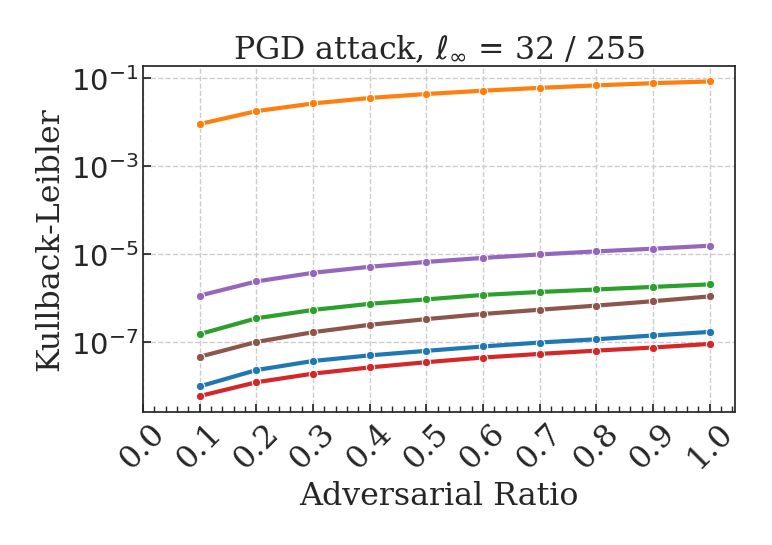
\includegraphics[width=\textwidth]{img/results_discussion/adversarial/PGD_KL.png}
    \end{subfigure}
    \hfill
    \begin{subfigure}[b]{0.45\textwidth}
        \centering
        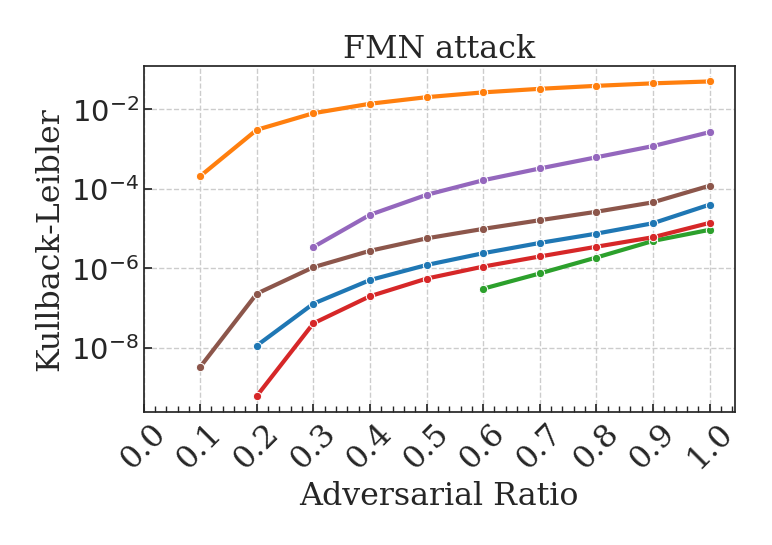
\includegraphics[width=\textwidth]{img/results_discussion/adversarial/FMN_KL.png}
    \end{subfigure}

    \vspace{1em}

    \begin{subfigure}[b]{0.45\textwidth}
        \centering
        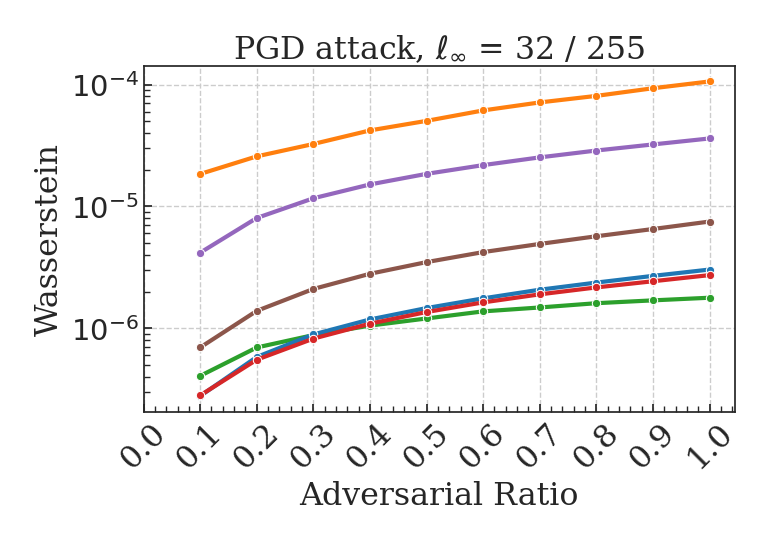
\includegraphics[width=\textwidth]{img/results_discussion/adversarial/PGD_W.png}
    \end{subfigure}
    \hfill
    \begin{subfigure}[b]{0.45\textwidth}
        \centering
        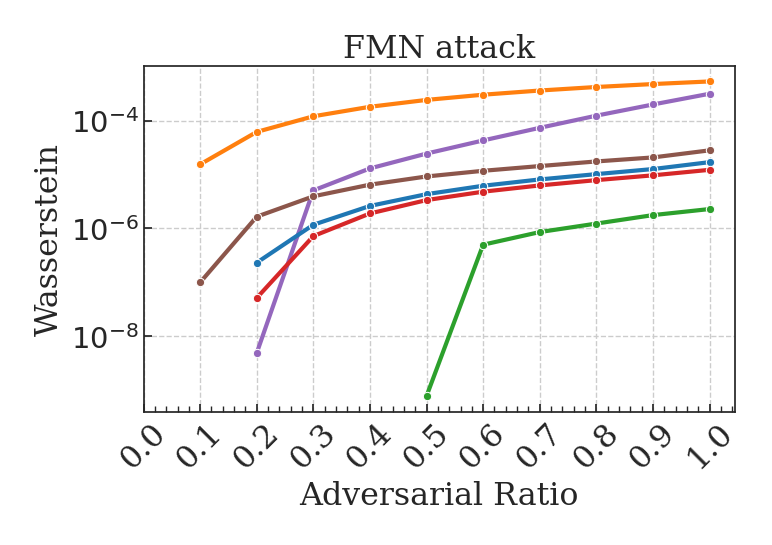
\includegraphics[width=\textwidth]{img/results_discussion/adversarial/FMN_W.png}
    \end{subfigure}

    \caption{Comparison using probability based distances.}
    \label{fig:six_figures}
\end{figure}

- As an alternative to posterior agreement we can try to infer robustness from the feature space (add here the right notation).
- For the FMN case they are not discriminative until a sufficiently high AR is achieved. Only when adversarial samples are labeled as such we could use these metrics (similar to anomaly detection) to assess similarity, but they would still be less informative about the feature space.

\begin{figure}[H]
    \centering
    \begin{subfigure}[b]{0.45\textwidth}
        \centering
        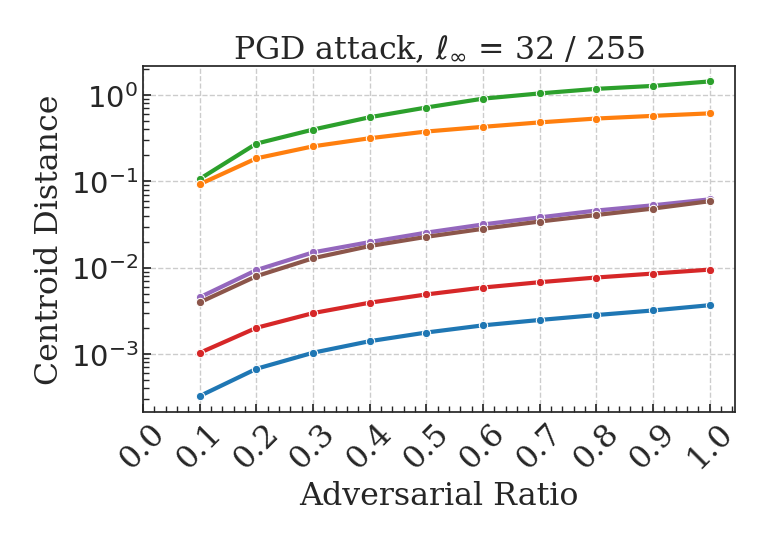
\includegraphics[width=\textwidth]{img/results_discussion/adversarial/PGD_CD.png}
    \end{subfigure}
    \hfill
    \begin{subfigure}[b]{0.45\textwidth}
        \centering
        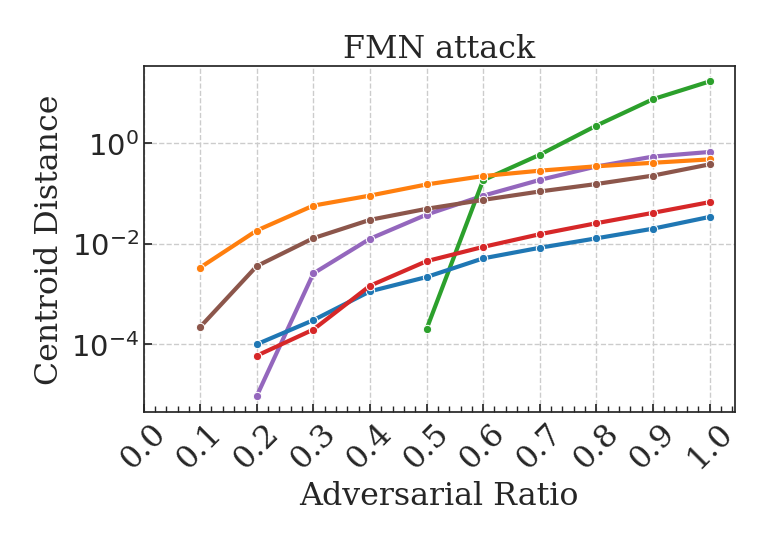
\includegraphics[width=\textwidth]{img/results_discussion/adversarial/FMN_CD.png}
    \end{subfigure}

    \vspace{1em}

    \begin{subfigure}[b]{0.45\textwidth}
        \centering
        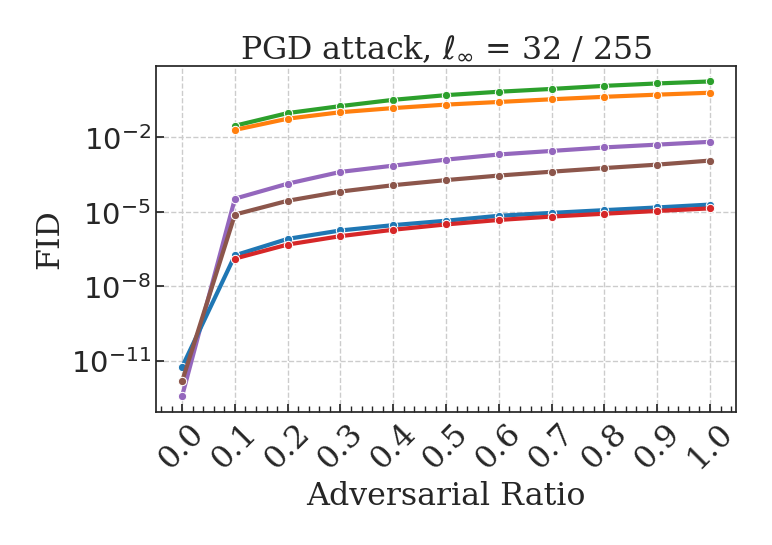
\includegraphics[width=\textwidth]{img/results_discussion/adversarial/PGD_FID.png}
    \end{subfigure}
    \hfill
    \begin{subfigure}[b]{0.45\textwidth}
        \centering
        \includegraphics[width=\textwidth]{img/results_discussion/adversarial/FMN_FID.png}
    \end{subfigure}

    \caption{Comparison using feature-space based distances.}
    \label{fig:six_figures}
\end{figure}



CLAIM: Robustness against increasing attack power

PROOF: Following plots. PA decreases with increasing attack power at AR=1.0.

- Only PA clearly discriminates BPDA from the rest of robust models. As explained before, this discrimination is fundamental and will be highly value in the domain generalization setting.
- The classical robustness definition discriminates the standard from the rest, as seen in DeltaAFR.
- For the reasons given before (peaked posterior distribution at betamax, etc), logPA is able to replicate the AFR (T) response.
- Feature space metrics show a constant increase of the distance between X and Xprime representations. The only model that does not follow the same trend is Standard, indicating that the feature space is not able to represent the shift represented by adversarial features.
- Posterior distance metrics discriminate also BPDA. In general, over increasing attack power, we see that feature-space and distribution-based distance metrics tend to behave differently. In all cases, they overfit to the increased distance existing between true and adversarial predictions in the red,blue model.



\begin{figure}[H]
    \centering
    \begin{subfigure}[b]{0.22\textwidth}
        \centering
        \includegraphics[width=\textwidth]{img/results_discussion/adversarial/PGD_CD_eps.png}
    \end{subfigure}
    \hfill
    \begin{subfigure}[b]{0.22\textwidth}
        \centering
        \includegraphics[width=\textwidth]{img/results_discussion/adversarial/PGD_FID_eps.png}
    \end{subfigure}
    \hfill
    \begin{subfigure}[b]{0.22\textwidth}
        \centering
        \includegraphics[width=\textwidth]{img/results_discussion/adversarial/PGD_KL_eps.png}
    \end{subfigure}
    \hfill
    \begin{subfigure}[b]{0.22\textwidth}
        \centering
        \vspace{-5pt}
        \includegraphics[width=\textwidth]{img/results_discussion/adversarial/PGD_W_eps.png}
    \end{subfigure}
    \caption{How metrics evolve with eps.}
    \label{fig:gaussian_optimization}
\end{figure}

This can be observed even more clearly on the gaussian attack. Both PA and AFR are able to select the Undefended model as the least robust one, in the sense that their predictions suffer greater change with increasing attack power. Nevertheless, PA is much more discriminative than

\begin{figure}[H]
    \centering
    \begin{subfigure}[b]{0.3\textwidth}
        \centering
        \includegraphics[width=\textwidth]{img/results_discussion/adversarial/GAUSSIAN_logPA_eps.png}
    \end{subfigure}
    \hfill
    \begin{subfigure}[b]{0.3\textwidth}
        \centering
        \includegraphics[width=\textwidth]{img/results_discussion/adversarial/GAUSSIAN_AFR_pred_eps.png}
    \end{subfigure}
    \hfill
    \begin{subfigure}[b]{0.3\textwidth}
        \centering
        \vspace{-5pt}
        \includegraphics[width=\textwidth]{img/results_discussion/adversarial/GAUSSIAN_AFR_true_eps.png}
    \end{subfigure}
    \caption{Evolution for eps.}
    \label{fig:gaussian_optimization}
\end{figure}

MISSING: MORE DIFFERENCE BETWEEN FMN AND PGD AT FUND. LEVEL.

\section{Domain generalization setting}\label{results_domain_generalization}


\begin{figure}[H]
    \centering
    \begin{subfigure}[b]{0.3\textwidth}
        \centering
        \includegraphics[width=\textwidth]{img/results_discussion/datashift/shift_ratio=0.200.pdf}
    \end{subfigure}
    \hfill
    \begin{subfigure}[b]{0.3\textwidth}
        \centering
        \includegraphics[width=\textwidth]{img/results_discussion/datashift/shift_ratio=0.400.pdf}
    \end{subfigure}
    \hfill
    \begin{subfigure}[b]{0.3\textwidth}
        \centering
        \includegraphics[width=\textwidth]{img/results_discussion/datashift/shift_ratio=0.600.pdf}
    \end{subfigure}

    \vspace{1em}

    \begin{subfigure}[b]{0.3\textwidth}
        \centering
        \includegraphics[width=\textwidth]{img/results_discussion/datashift/shift_ratio=0.800.pdf}
    \end{subfigure}
    \hspace{13pt}
    \begin{subfigure}[b]{0.3\textwidth}
        \centering
        \includegraphics[width=\textwidth]{img/results_discussion/datashift/shift_ratio=1.000.pdf}
    \end{subfigure}

    \caption{Datashift for paper.}
    \label{fig:six_figures}
\end{figure}

- Adam was used to avoid a continuous pathway in the optimization landscape and therefore favouring the exploration of different solutions that might generalize better to increasingly shifted datasets.
- PA is a lower bound for accuracy, in the sense tha t

\begin{figure}[H]
    \centering
    \begin{subfigure}[b]{0.45\textwidth}
        \centering
        \includegraphics[width=\textwidth]{img/results_discussion/datashift/paper_oracle_all_erm.png}
    \end{subfigure}
    \hfill
    \begin{subfigure}[b]{0.45\textwidth}
        \centering
        \includegraphics[width=\textwidth]{img/results_discussion/datashift/paper_PA_all_erm.png}
    \end{subfigure}

    \vspace{1em}

    \begin{subfigure}[b]{0.45\textwidth}
        \centering
        \includegraphics[width=\textwidth]{img/results_discussion/datashift/paper_oracle_all_irm.png}
    \end{subfigure}
    \hfill
    \begin{subfigure}[b]{0.45\textwidth}
        \centering
        \includegraphics[width=\textwidth]{img/results_discussion/datashift/paper_PA_all_irm.png}
    \end{subfigure}

    \caption{PA evaluation.}
    \label{fig:six_figures}
\end{figure}

\begin{figure}
    \centering
    \includegraphics[width=0.7\textwidth]{img/results_discussion/datashift/model_selection.png}
    \caption{Model selection capabilities.}
    \label{fig:model_selection_capabilities}
\end{figure}

\begin{figure}[H]
    \centering
    \begin{subfigure}[b]{0.32\textwidth}
        \centering
        \includegraphics[width=\textwidth]{img/results_discussion/datashift/paper_selection_ppred=1.0_met=acc.png}
    \end{subfigure}
    \hfill
    \begin{subfigure}[b]{0.32\textwidth}
        \centering
        \includegraphics[width=\textwidth]{img/results_discussion/datashift/paper_selection_ppred=1.0_met=sensitivity.png}
    \end{subfigure}
    \hfill
    \begin{subfigure}[b]{0.32\textwidth}
        \centering
        \vspace{-5pt}
        \includegraphics[width=\textwidth]{img/results_discussion/datashift/paper_selection_ppred=1.0_met=specificity.png}
    \end{subfigure}
    \caption{Model selection for \texttt{paper}.}
    \label{fig:gaussian_optimization}
\end{figure}



\cleardoublepage


\chapter{Discussion}\label{sec:again_something}

Blah, blah \dots

 \cleardoublepage

\cleardoublepage

% \chapter{Blabla}\label{sec:blabla}

\section{References and Footnotes}\label{sec:references}
References to literature are included using the command \texttt{\textbackslash
cite\{.\}}. For example \cite{optreg,motsys}. Your references must be entered in the file \texttt{bibliography.bib}. Making changes or adding new references in the bibliography file can be done manually or by using specialized software such as \textit{JabRef} which is free of charge.
 
Cross-referencing within the text is easily done using \texttt{\textbackslash label\{.\}} and \texttt{\textbackslash ref\{.\}}. For example, this paragraph is part of chapter~\ref{sec:working}; more specifically section~\ref{sec:references} on page~\pageref{sec:references}. You will need to compile your document twice in order for the cross-referencing to be updated.

Footnotes\footnote{The use of footnotes is generally not recommended.} are added using the command \texttt{\textbackslash footnote\{.\}}, but try to avoid the used of footnotes altogether.

\section{Lists}\label{sec:lists}
Three types of list-environments are commonly used: \texttt{itemize}, \texttt{enumerate}, and \texttt{description}. The following example uses \texttt{itemize} to create a list without numbering
\begin{itemize}
  \item point one; and
  \item point two
\end{itemize}
created using
\begin{verbatim}
\begin{itemize}
  \item point one; and
  \item point two
\end{itemize}
\end{verbatim}

The following example uses \texttt{enumerate} to create a list with numbering
\begin{enumerate}
  \item point one; and
  \item point two
\end{enumerate}
created using
\begin{verbatim}
\begin{enumerate}
  \item point one; and
  \item point two
\end{enumerate}
\end{verbatim}

The following example uses \texttt{description} to create a list with custom text as bullet-points
\begin{description}
  \item[P1] point one; and
  \item[P2] point two
\end{description}
created using
\begin{verbatim}
\begin{description}
  \item[P1] point one; and
  \item[P2] point two
\end{description}
\end{verbatim}


\section{Tables}\label{sec:tables}
Table~\ref{tab:table} shows an example of a simple table-layout. Try to avoid vertical lines on tables. The Internet contains countless resources on how to create special elements and structures in tables such as cells spanning multiple rows, rotated text, sideways tables, justification of cell elements, etc.
\begin{table}[ht]
\begin{center}
\caption{Driving cycle data of ECE-15, EUDC, and NEDC.}\vspace{1ex}
\label{tab:table}
\begin{tabular}{llccc}\hline
Description & Unit & ECE & EUDC & NEDC \\ \hline
Duration & s & 780 & 400 & 1180 \\
Distance & km & 4.052 & 6.955 & 11.007 \\
Average velocity & km/h & 18.7 &  62.6 & 33.6 \\
Idle speed & \% & 36 & 10 & 27 \\ \hline
\end{tabular}
\end{center}
\end{table}

This table was created using
\begin{verbatim}
\begin{table}[ht]
\begin{center}
\caption{Driving cycle data of ECE-15, EUDC, and NEDC.}\vspace{1ex}
\label{tab:table}
\begin{tabular}{llccc}\hline
Description & Unit & ECE & EUDC & NEDC \\ \hline
Duration & s & 780 & 400 & 1180 \\
Distance & km & 4.052 & 6.955 & 11.007 \\
Average velocity & km/h & 18.7 &  62.6 & 33.6 \\
Idle speed & \% & 36 & 10 & 27 \\ \hline
\end{tabular}
\end{center}
\end{table}
\end{verbatim}
Table~\ref{tab:table_advanced} shows a more advanced version of Tab.~\ref{tab:table} using the \texttt{booktabs} package. Inspect the source code of this document to see how this was done.
\begin{table}[ht]
\begin{center}
\small
\caption{Driving cycle data of ECE-15, EUDC, and NEDC.}\vspace{1ex}
\label{tab:table_advanced}
\begin{tabular}{@{}lcccc@{}}\toprule[1.5pt]
& & \multicolumn{3}{c}{\bf Driving cycle}\\
\cmidrule{3-5}
Description & Unit & {ECE} & {EUDC} & {NEDC} \\ \midrule
Duration & \unit[]{s} & 780 & 400 & 1180 \\
Distance & \unit[]{km} & 4.052 & 6.955 & 11.007 \\
Average velocity & \unitfrac[]{km}{h} & 18.7 &  62.6 & 33.6 \\
Idle speed & \unit[]{\%} & 36 & 10 & 27 \\ \bottomrule[1.5pt]
\end{tabular}
\end{center}
\end{table}



\section{Working with Units}
The package \texttt{\textbackslash usepackage\{units\}} enables two useful commands, namely \texttt{\textbackslash unit[.]\{.\}} and \\ \texttt{\textbackslash unitfrac[.]\{.\}\{.\}}. Use these commands to display units in a concise way, for example
\begin{align}
\delta t &= \unit[1]{s}\\
v &= \unitfrac[5]{m}{s}.
\end{align}
This example was done using
\begin{verbatim}
\begin{align}
\delta t &= \unit[1]{s}\\
v &= \unitfrac[5]{m}{s}.
\end{align}
\end{verbatim}

\section{Including Graphics}\label{sec:epsgraph}
It is recommended that you only use encapsulated post-script graphics \texttt{.eps} in your report. If you mix \texttt{.eps} with other formats such as \texttt{.png}, \texttt{.jpeg} or \texttt{.gif}, you will most likely not be able to compile your report without errors. Note that figures created in \textsc{Matlab} are easily saved in \texttt{.eps} format.

The inclusion of a figure can be done in the following way:
\begin{verbatim}
\begin{figure}[ht]
   \centering
   \includegraphics[width=0.75\textwidth]{img/k_surf.eps}
   \caption{Example of a figure.}
   \label{img:k_surf}
\end{figure}
\end{verbatim}

\begin{figure}[ht]
   \centering
   \includegraphics[width=0.75\textwidth]{img/k_surf.eps}
   \caption{Example of a figure.}
   \label{img:k_surf}
\end{figure}

Two figures are displayed next to each other using
\begin{verbatim}
\begin{figure}[ht]
  \begin{minipage}[t]{0.48\textwidth}
    \includegraphics[width = \textwidth]{img/cycle_we.eps}
  \end{minipage}
  \hfill
  \begin{minipage}[t]{0.48\textwidth}
    \includegraphics[width = \textwidth]{img/cycle_ml.eps}
  \end{minipage}
  \caption{Two figures next to each other.}
  \label{img:cycle}
\end{figure}
\end{verbatim}

\begin{figure}[ht]
  \begin{minipage}[t]{0.48\textwidth}
    \includegraphics[width = \textwidth]{img/cycle_we.eps}
  \end{minipage}
  \hfill
  \begin{minipage}[t]{0.48\textwidth}
    \includegraphics[width = \textwidth]{img/cycle_ml.eps}
  \end{minipage}
  \caption{Two figures next to each other.}
  \label{img:cycle}
\end{figure}

The positioning parameter \texttt{h} (here) forces your figure to be placed in the current position relative to your text. You may add \texttt{t} (top), \texttt{b} (bottom), and/or \texttt{p} (page) to allow for more flexible positioning within your document. For instance, \texttt{[tb]} forces your figure to be placed either on the top or bottom of a page.


\section{Equations}\label{sec:math}
The most common way to include equations is using the \texttt{equation} environment.
\begin{equation}\label{eq:p_me0f}
 p_\mathrm{me0f}(T_e,\omega_e) \ = \ k_1(T_e) \cdot (k_2+k_3 S^2
 \omega_e^2) \cdot \Pi_\mathrm{max} \cdot \sqrt{\frac{k_4}{B}} \, .
\end{equation}
It is recommended to use \texttt{\textbackslash mathrm\{.\}} for subscripts comprising more than two letters since it reduces the width of the subscript significantly and improves readability. The corresponding code is
\begin{verbatim}
\begin{equation}\label{eq:p_me0f}
 p_\mathrm{me0f}(T_e,\omega_e) \ = \ k_1(T_e) \cdot (k_2+k_3 S^2
 \omega_e^2) \cdot \Pi_\mathrm{max} \cdot \sqrt{\frac{k_4}{B}} \, .
\end{equation}
\end{verbatim}
Equations, such as Eq.~\eqref{eq:p_me0f}, may be referenced using \texttt{\textbackslash eqref\{.\}}. In-line mathematical content is created using \texttt{\$.\$}, for example $a^2+b^2=c^2$. It is practically possible to typeset any equation in \LaTeX. Equation~\eqref{eq:advanced} shows an example of a more advance structure.
\begin{equation}\label{eq:advanced}
x^k_n(i) = \left\{\begin{array}{ll}y(i) & \text{if}\quad x^k_{n-1}(i)\leq \mathbf{x}\\
z(i) & \text{otherwise}\end{array}\right., \text{for}\quad i=\{1,\ldots,N\}.
\end{equation}



\section{Including Code in your Document}
Include samples from your Matlab code using the \texttt{lstlistings} environment, for example
\lstset{language=Matlab,numbers=none}
\begin{lstlisting}[frame=lines]
% Evaluate y = 2x
for i = 1:length(x)

  y(i) = 2*x(i);

end
\end{lstlisting}
This example was created using
\begin{verbatim}
\lstset{language=Matlab,numbers=none}
\begin{lstlisting}[frame=lines]
% Evaluate y = 2x
for i = 1:length(x)

  y(i) = 2*x(i);

end
\end{lstlisting}
\end{verbatim}
where \texttt{\textbackslash usepackage\{mcode\}} must be included in the preamble of your document. If you want to include the entire content of a file \texttt{mycode.m} in your document, simply input the path to \texttt{mycode.m} instead of pasting the entire content into your \TeX -file
\begin{verbatim}
\lstset{language=Matlab,numbers=left}
\lstinputlisting{path/to/mycode.m}
\end{verbatim}
Including the path to your m-file also ensures that the code in your report is always up-to-date. The \texttt{\textbackslash lstset\{language=Matlab\}} command ensures that \textsc{Matlab} syntax definitions are used, but many other languages are recognised as well such as \texttt{Fortran} and \texttt{C++}.

% \cleardoublepage

% \input{}
% \cleardoublepage
% \input{}
% \cleardoublepage
% ...

% Appendix______________________________________________________________________
\appendix
\chapter{Supplementary material}\label{sec:something}

We will define some notation shortcuts for the following proofs.



\section{Proof of problem formulation}\label{sec:proofs}

\begin{lemma} 
    
    Let $N, K \in \mathbb{N}$ and let $\left\{\mathcal{E}_{i j} \mid i \leq N, j \leq K\right\}$ be an indexed set of values. Then,
    $$
    \sum_{c \in \mathcal{C}} \prod_{i=1}^N \mathcal{E}_{i, c(i)}=\prod_{i=1}^N \sum_{j=1}^K \mathcal{E}_{i j}
    $$
\end{lemma}

\begin{proof}
By induction on $N$. For the $N=1$ base case, observe that $\mathcal{C}$ has only $K$ elements, as there are only $K$ functions mapping $\{1\}$ to $\{1, \ldots, K\}$. Then
$$
\sum_{c \in \mathcal{C}} \prod_{i \leq N} \mathcal{E}_{i, c(i)}=\sum_{c \in \mathcal{C}} \mathcal{E}_{1, c(1)}=\sum_{j \leq K} \mathcal{E}_{1, j}=\prod_{i \leq N} \sum_{j \leq K} \mathcal{E}_{i, j} .
$$

Assume now that the result holds for some $N$. We demonstrate then that it also holds for $N+1$. Observe that there is a bijection between $\mathcal{C}$ and $\{1, \ldots, K\}^N$. Therefore, we identify every function $c \in \mathcal{C}$ with the tuple $(c(1), \ldots, c(N))$. Conversely, we identify every tuple $\left(c_1, \ldots, c_N\right) \in\{1, \ldots, K\}^N$, with the function $c$ that maps $i$ to $c_i$.

$$
\begin{aligned}
    & \sum_{c \in \mathcal{C}} \prod_{i \leq N+1} \mathcal{E}_{i, c(i)}= \\
    & =\sum_{\left(c_1, \ldots, c_{N+1}\right) \in\{1, \ldots, K\}^{N+1}} \prod_{i \leq N+1} \mathcal{E}_{i, c_i} \\
    & =\sum_{\substack{\left(c_1, \ldots, c_N\right) \in\{1, \ldots, K\}^N \\
    c_{N+1} \leq K}} \prod_{i \leq N+1} \mathcal{E}_{i, c_i} \\
    & =\sum_{\left(c_1, \ldots, c_N\right) \in\{1, \ldots, K\}^N} \sum_{c_{N+1} \leq K} \prod_{i \leq N+1} \mathcal{E}_{i, c_i} \\
    & =\sum_{\left(c_1, \ldots, c_N\right) \in\{1, \ldots, K\}^N} \sum_{c_{N+1} \leq K}\left(\mathcal{E}_{N+1, c(N+1)} \prod_{i \leq N} \mathcal{E}_{i, c_i}\right) \\
    & =\left(\sum_{c_{N+1} \leq K} \mathcal{E}_{N+1, c(N+1)}\right) \sum_{\left(c_1, \ldots, c_N\right) \in\{1, \ldots, K\}^N} \prod_{i \leq N} \mathcal{E}_{i, c_i} \\
    & =\left(\sum_{c_{N+1} \leq K} \mathcal{E}_{N+1, c(N+1)}\right) \prod_{i \leq N} \sum_{j \leq K} \mathcal{E}_{i, j} \\
    & =\left(\sum_{j \leq K} \mathcal{E}_{N+1, j}\right) \prod_{i \leq N} \sum_{j \leq K} \mathcal{E}_{i, j} \\
    & =\prod_{i \leq N+1} \sum_{j \leq K} \mathcal{E}_{i, j} . \\
    &
    \end{aligned}
$$
\end{proof}


\begin{theorem}[Posterior factorization]

    The posterior distribution for a classification problem can be factorized as follows:
    $$
    \mathbf{P}^c(\theta \mid \bm{x}) = \prod_i^N  \mathbf{P}^c(\theta_i \mid \bm{x}) = \prod_{i=1}^N \frac{\exp \left ( \beta F_{\theta_i}(x_i) \right )}{\sum_{j=1}^K \exp \left ( \beta F_j(x_i) \right )}
    $$
\end{theorem}

\begin{proof}
    The posterior distribution solution to the MAP problem is the following:

    $$
    \mathbf{P}^c(\theta \mid \bm{x}) \frac{\exp \left ( \beta \sum_{i=1}^N F_{\theta_i}(x_i) \right )}{\sum_{\theta \in \Theta} \exp \left ( \beta \sum_{i=1}^N F_{\theta_i}(x_i) \right )}
    = \frac{\prod_{i=1}^N \exp \left ( \beta F_{\theta_i}(x_i) \right )}{\sum_{\theta \in \Theta} \prod_{i=1}^N \exp \left ( \beta  F_{\theta_i}(x_i) \right )}
    $$

    Using Lemma \ref{lemma:exchangeability} we can rewrite the denominator as:

    $$
    \sum_{\theta \in \Theta} \prod_{i=1}^N \exp \left ( \beta  F_{\theta_i}(x_i) \right ) = \prod_{i=1}^N \sum_{\theta \in \Theta} \exp \left ( \beta  F_{\theta_i}(x_i) \right )
    $$

    Therefore, the posterior distribution can be written as:

    $$
    \mathbf{P}^c(\theta \mid \bm{x}) = \prod_{i=1}^N  \mathbf{P}^c(\theta_i \mid \bm{x}) = \prod_{i=1}^N \frac{\exp \left ( \beta F_{\theta_i}(x_i) \right )}{\sum_{\theta \in \Theta} \exp \left ( \beta R(\theta, \bm{x}) \right )}
    $$

\end{proof}

\section{Properties of the PA kernel}\label{sec:kernel}

\begin{theorem}[Symmetry of the PA kernel]
    The posterior agreement kernel is symmetric with respect to the definition of $X'$ and $X''$.

    $$
    PA(\bm{x}', \bm{x}'') = PA(\bm{x}'', \bm{x}')
    $$
\end{theorem}

\begin{theorem}[Non-negativity of the PA kernel]
    The posterior agreement kernel is non-negative.

    $$
    PA(\bm{x}', \bm{x}'') \geq 0
    $$  
\end{theorem}

\begin{theorem}[Concavity of the PA kernel]
    The posterior agreement kernel is concave in $\mathbb{R}^+$, and therefore
    has a unique maximum.
\end{theorem}

\begin{proof}

The posterior agreement kernel has been shown to have the following form:

$$
\operatorname{PA}\left(\bm{x}', \bm{x}'' \right) \propto \sum_{n=1}^N \log \left[ \sum_{j=1}^K \mathbf{P}_n^c(\theta \mid x_n') \mathbf{P}_n^c(\theta \mid x_n'') \right]
$$

where the posteriors $\mathbf{P}_n^c(\theta \mid x_n)$ are Gibbs distributions for each observation.

$$
\mathbf{P}_n^c(\theta \mid x_n') = \frac{e^{\beta F_j(x_n)}}{\sum_{k=1}^K e^{\beta F_k(x_n)}}
$$

We will require three important results from optimization theory:

\begin{description}
    \item[T1] The minimum of $G(\beta) = -\operatorname{PA}(X', X'')$ over the convex set $\mathbb{R}^+$ is unique $\iff$ $G(\beta)$ is convex.
    \item[T2] $G$ is absolutely convex $\iff$ $\frac{d^2}{d \beta^2} G(\beta) > 0$.
    \item[T3] The sum of convex functions is also convex.
\end{description}


To streamline the derivation, the following notation will be used:

$$
F_j(x_n') = F'_j
$$

$$
e^{\beta F_j(x_n')} = e^{\beta F'_j} = e'_j
$$

The observation index $n$ will be omitted as it does not affect the convexity derivation (see \textbf{T3}). With that notation in mind, we can define $G(\beta)$ properly:

$$
G(\beta) = -k(\bm{x}', \bm{x}'') = \sum_{n=1}^N - \log \left [\sum_{j=1}^K e'_j e''_j \right] + \sum_{n=1}^N \log \left [ \sum_{k=1}^K e'_k \sum_{p=1}^K e''_p \right] 
$$

We will focus on the first term: $G^n_1(\beta) = G_1(\beta) = \log \left [\sum_{j=1}^K e'_j e''_j \right]$.

$$
\frac{d}{d \beta} G_1(\beta) = \frac{\sum_{j=1}^K (F'_j + F''_j)e'_j e''_j }{\sum_{j=1}^K e'_j e''_j }
$$

The derivative $\frac{d}{d \beta} e'_j e''_k$ will be used recurrently in this section:

$$
\frac{d}{d \beta} e'_j e''_k = F'_j e'_j e''_k +e'_j F''_k  e''_k = (F'_j + F''_k) e'_j e''_k
$$

The second derivative is straightforward:

$$
\frac{d^2}{d \beta ^2} G_1(\beta) = \frac{\sum_{j=1}^K (F'_j + F''_j)^2 e'_j e''_j }{\sum_{j=1}^K e'_j e''_j } - \frac{\left (\sum_{j=1}^K (F'_j + F''_j) e'_j e''_j \right ) ^2}{\left (\sum_{j=1}^K e'_j e''_j \right )^2}
$$

We impose the convexity condition and see whether it can be contradicted.

$$
\frac{d^2}{d \beta ^2} G_1(\beta) > 0 \iff \left(\sum_{j=1}^K e'_j e''_j \right ) \left( \sum_{j=1}^K (F'_j + F''_j)^2 e'_j e''_j  \right ) - \left (\sum_{j=1}^K (F'_j + F''_j) e'_j e''_j \right )^2 > 0
$$

Using the distributive property of the product over the sum, we can reindex our expression:

$$
\sum_{k=1}^K \sum_{j=1}^K (F'_j + F''_j)^2 e'_j e''_j e'_k e''_k - \sum_{k=1}^K \sum_{j=1}^K (F'_j + F''_j) (F'_k + F''_k) e'_j e''_j e'_k e''_k > 0 \iff
$$

$$
\iff \sum_{k=1}^K \sum_{j=1}^K [(F'_j + F''_j) - (F'_k + F''_k) ] (F'_j + F''_j) e'_j e''_j e'_k e''_k  > 0
$$

As we can see, $\Delta_{(jj), (kk)} $ corresponds to the difference in the cost attributed to reference class $j$ and the cost attributed to class $k$, accumulated over $\bm{x}', \bm{x}''$. We can intuitively devise some symmetry in these terms, and we formalize it as follows:

$$
E_{jk} = e'_j e''_j e'_k e''_k = E_{kj}
$$

$$
\Delta_{(jj), (kk)} = (F'_j + F''_j) - (F'_k + F''_k) = (F'_j - F'_k) + (F''_j - F''_k) = - \Delta_{(kk), (jj)}
$$

 Even if $\Delta_{(jj), (jj)} = 0$, we will still include this term to facilitate with the indexing. Overall, the sum can be expressed as:

$$
 \sum_{k=1}^K \sum_{j=1}^K [(F'_j + F''_j) - (F'_k + F''_k) ] (F'_j + F''_j) e'_j e''_j e'_k e''_k = \sum_{k=1}^K \sum_{j=1}^K (F'_j + F''_j) E_{jk} \Delta_{(jj), (kk)} = \sum_{k=1}^K \sum_{j=1}^K S_{(jj), (kk)}
$$


Then, the pairwise sum of symmetric combinations of indexes $k$ and $j$ yields

$$
\begin{aligned}
    S_{(jj), (kk)} + S_{(kk), (jj)} & = (F'_j + F''_j) E_{jk} \Delta_{(jj), (kk)} + (F'_k + F''_k) E_{kj} \Delta_{(kk), (jj)} \\
    & = E_{jk}\Delta_{(jj), (kk)} [(F'_j + F''_j) - (F'_k + F''_k)] = E_{jk}\Delta_{(jj), (kk)}^2 > 0
\end{aligned}
$$


Given that the indexing sets in our nested sum are the same, it's straightforward to see that all the terms will be strictly positive, and the overall sum will be zero only if $e_j = 0 \; \forall j=\{ 1,...K \}$, which is not possible in a classification setting since $\beta \in \mathbb{R}^+$. We end up with the following expression:

$$
\frac{d^2}{d \beta ^2} G_1(\beta) = \sum_{k=1}^K \sum_{j<k}^K E_{jk}\Delta_{(jj), (kk)}^2 > 0
$$

Now we proceed analogously with the second term: 

$$
G^n_2(\beta) = G_2(\beta) = \log \left [\sum_{j=1}^K e'_j \sum_{k=1}^K e''_k \right] = \log \left [\sum_{k=1}^K \sum_{j=1}^K e'_j e''_k \right]
$$

$$
\frac{d}{d \beta} G_2(\beta) = \frac{\sum_{k=1}^K \sum_{j=1}^K (F'_j + F''_k) e'_j e''_k}{\sum_{k=1}^K \sum_{j=1}^K e'_j e''_k}
$$

$$
\frac{d^2}{d^2 \beta} G_2(\beta) = \frac{\sum_{k=1}^K \sum_{j=1}^K (F'_j + F''_k)^2 e'_j e''_k}{\sum_{k=1}^K \sum_{j=1}^K e'_j e''_k} - \frac{\left(\sum_{k=1}^K \sum_{j=1}^K (F'_j + F''_k) e'_j e''_k \right)^2}{\left( \sum_{k=1}^K \sum_{j=1}^K e'_j e''_k\right)^2} > 0 \iff
$$
$$
\iff \left(\sum_{k=1}^K \sum_{j=1}^K e'_j e''_k \right) \left(\sum_{k=1}^K \sum_{j=1}^K (F'_j + F''_k)^2 e'_j e''_k \right) - \left(\sum_{k=1}^K \sum_{j=1}^K (F'_j + F''_k) e'_j e''_k \right)^2 > 0 \iff
$$
$$
\iff \sum_{k=1}^K \sum_{q=1}^K \sum_{j=1}^K \sum_{i=1}^K (F'_j + F''_k)^2 e'_j e''_k e'_i e''_q - (F'_j + F''_k) e'_j e''_k (F'_i + F''_q) e'_i e''_q > 0 \iff
$$
$$
\iff \sum_{k=1}^K \sum_{q=1}^K \sum_{j=1}^K \sum_{i=1}^K (F'_j + F''_k) e'_j e''_k e'_i e''_q [(F'_j + F''_k) - (F'_i + F''_q)] > 0
$$

We can define as well:

$$
\frac{d^2}{d^2 \beta} G_2(\beta) = \sum_{k=1}^K \sum_{q=1}^K \sum_{j=1}^K \sum_{i=1}^K S_{(jk),(iq)} = \sum_{k=1}^K \sum_{q=1}^K \sum_{j=1}^K \sum_{i=1}^K (F'_j + F''_k) E_{(jk),(iq)} \Delta_{(jk),(iq)} 
$$

$$
E_{(jk),(iq)} = e'_j e''_k e'_i e''_q = E_{(ik),(jq)} = E_{(jq),(ik)} = E_{(iq),(jk)}
$$

$$
\Delta_{(jk),(iq)} = (F'_j - F'_i) + (F''_k - F''_q) = - \Delta_{(iq),(jk)}
$$

The symmetry arises when adding two elements that have mirror indexes in both $\bm{x}'$ and $\bm{x}''$.

$$
\begin{aligned}
S_{(jk),(iq)} + S_{(iq),(jk)} & = (F'_j + F''_k) E_{(jk),(iq)} \Delta_{(jk),(iq)} + (F'_i + F''_q) E_{(iq),(jk)} \Delta_{(iq),(jk)} \\
& = E_{(jk),(iq)} \Delta_{(jk),(iq)} [(F'_j + F''_k) - (F'_i + F''_q)] = E_{(jk),(iq)} \Delta_{(jk),(iq)}^2 > 0
\end{aligned}
$$

Given that symmetries are independent for $\bm{x}'$ and $\bm{x}''$, we end up with a similar expression:

$$
\frac{d^2}{d \beta ^2} G_2(\beta) = \sum_{k=1}^K \sum_{q<k}^K \sum_{j=1}^K \sum_{i<j}^K E_{(jk),(iq)}\Delta_{(jk),(iq)}^2 > 0
$$

Even if a further simplified version can be obtained, this one will allow us to complete the proof. We can now define the function $G(\beta)$ as the sum of the two terms:

$$
\frac{d^2}{d \beta ^2} G(\beta) = \sum_{n=1}^N \left [ \sum_{k=1}^K \sum_{q<k}^K \sum_{j=1}^K \sum_{i<j}^K E_{(jk),(iq)}\Delta_{(jk),(iq)}^2 - \sum_{k=1}^K \sum_{q<k}^K E_{(qq), (kk)}\Delta_{(qq), (kk)}^2 \right ]
$$

where we can clearly see that the particular case $\{ k=j, q=i \}$ cancels the negative terms:

$$
\begin{aligned}
    \frac{d^2}{d \beta ^2} F^n(\beta) & = \sum_{k=1}^K \sum_{q<k}^K \sum_{j = \{ 1:K \} \setminus \{ k \} } \sum_{i = \{ 1:K | i < j\} \setminus \{ k \} } E_{(jk),(iq)}\Delta_{(jk),(iq)}^2  \\ 
    & + \sum_{k=1}^K \sum_{q<k}^K E_{(qq), (kk)}\Delta_{(qq), (kk)}^2 - \sum_{k=1}^K \sum_{q<k}^K E_{(qq), (kk)}\Delta_{(qq), (kk)}^2 = \\
    & = \sum_{k=1}^K \sum_{q<k}^K \sum_{j = \{ 1:K \} \setminus \{ k \} } \sum_{i = \{ 1:K | i < j\} \setminus \{ k \} } E_{(jk),(iq)}\Delta_{(jk),(iq)}^2 > 0
\end{aligned}
$$

Which proves that $G(\beta)$ is absolutely convex in $\mathbb{R}^+$:

$$
 \frac{d^2}{d \beta ^2} G(\beta) = \sum_{n=1}^N \frac{d^2}{d \beta ^2} G^n(\beta) = \sum_{n=1}^N \left[ \sum_{k=1}^K \sum_{q<k}^K \sum_{j = \{ 1:K \} \setminus \{ k \} } \sum_{i = \{ 1:K | i < j\} \setminus \{ k \} } E_{(jk),(iq)}\Delta_{(jk),(iq)}^2 \right] > 0
$$

We must note that on the limit $\beta \to \infty$ the curvature is not defined, so it will be always a good practice to start the numerical procedure at a value $\beta_0 = 0^+$:

$$
\lim_{\beta \to 0^+} \frac{d^2}{d \beta ^2} G(\beta) > 0
$$

\end{proof}

\cleardoublepage


\chapter{Again Something}\label{sec:again_something}

Blah, blah \dots

 \cleardoublepage



% Bibliography__________________________________________________________________
% Literature (Additional references can be added to the .bib-file manually, or by using, for example, the free application JabRef). Compile in the following order: latex -bibtex -latex -latex

\bibliographystyle{plain}
\bibliography{bibliography}

\end{document}
